\documentclass{llncs}
\usepackage{llncsdoc}

\intextsep=0.6\intextsep
\textfloatsep=0.6\textfloatsep
\abovecaptionskip=0.6\abovecaptionskip
\belowcaptionskip=0.6\belowcaptionskip

\usepackage{graphicx,amsfonts,amssymb,url,float,verbatim,listings,courier,pgfplots,tikz,tikzscale}
\usetikzlibrary{arrows}
\usetikzlibrary{positioning}
\pgfplotsset{compat=newest}

\title{Nibbles and bytes: an implementation of the trie data structure using different branching factors}

\author{Alex Schultz}

\institute{Tufts University}

\begin{document}

\maketitle

\begin{abstract}
This project consists of an implementation of the trie data structure that, instead of considering input strings character by character, considers input strings in chunks of one, two, four, or eight bits uniformly through the trie. The purpose of this was twofold: to complete a trie library that is able to work on arbitrary length input, and to do some simple testing of the behavior of the tries that use differing internal chunk sizes while working with the same data set. The C programming language was chosen for the ease it provides when working on individual bits in memory, which was necessary for this project.
\end{abstract}

\section{Introduction and Background}
\label{Introduction and Background}
When storing data in a program, a programmer may opt to use a few different structures, depending on the type of data and other constraints. For many common use cases, it does not matter which data structure the programmer chooses to use. The main requirement that is placed upon the data structure is that it be easy to use (so that including it in the program, or allowing others to access it, does not unnecessarily burden the programmer). In addition, its performance must be consistently good under normal circumstances (that is, outside of contrived examples that cause degraded performance that may nevertheless be useful in certain cases, such as to illustrate trade-offs between different data structures). Optionally, it may also be necessary that its design fits the needs of the programmer (consider the difference between a last in, first out (LIFO) structure like a stack and a first in, first out (FIFO) structure like a queue). On the last point, the optional part comes from the fact that in some circumstances, a simple array will be fine for a program, but in others, some kind of ordering (as in a queue) or mapping (as in a hash table) may be desired. \\

While a trie can be used to simply contain elements (in the same way a set or multiset would, but allowing in-order traversal like an ordered list would), a trie can also be used to map elements to one another, as a hash table would be used for. One of the reasons to use a trie over another data structure is that certain basic operations (search, insert, delete) can be done in time proportional to the length of the input data, rather than being done in time proportional to the amount of data already in the data structure. This is the case with some other tree data structures, which, depending on the use case, may be important when timing is of utmost importance. \\

A trie is a specific type of tree where each node stores part of the input data. For example, if one were to input the string 'dog' into an empty trie, the three nodes 'd', 'o', and 'g' would be placed in that order hierarchically, with the 'g' node marked as an endpoint node. If one were to then add the string 'don' into that trie, the only change would be the addition of a 'n' node (marked as an endpoint) as a child of the existing 'o' node - essentially, the path of nodes created by travelling from the root to a marked node forms an input string in the trie. To further this example, adding the string 'do' to the tree would simply mark the existing 'o' node as an endpoint, with no further consumption of space. In this way, for sets of strings that share prefixes, space is used very efficiently as only a single copy of the shared common prefix of the string needs to be stored, rather than storing a copy of that shared prefix for each entry in the set that is stored in the trie. \\ 
\begin{center}
\includegraphics[width=\linewidth,height=0.5\linewidth]{example_trie.tex.tikz}
\\
Trie states after adding the strings 'dog', 'don', and 'do'.\\
Endpoints are darkened.\\
\end{center}
In this implementation of the trie data structure, which takes in strings of bits as input, the tries created can be of four types: bytewise, nibblewise (half byte; four bits), doublebitwise, or bitwise. In each case, the number of bits held at each node in the trie is noted in the name - for example, the nibblewise trie would hold four bits in each node, while the doublebitwise trie would hold two bits in each node. For the tree mentioned above, each node held exactly one character of the inserted string. In the implementation of tries that this project has created, that association of one character per node would be equivalent to bytewise trie, since we are using C strings with one byte per character. \\
There are three operations done against a trie: insert a string into the trie, check whether a string exists in the trie, or delete a string from the trie. In the case of inserting a string of bits into a trie, we first partition the input string into chunks of a length based on the trie. For example, in a bytewise trie, each chunk would be exactly eight bits in size. From those chunks, we walk the trie by going through each chunk and placing it in the trie if needed. For each node n we walk to, the child node we move to from node n is the child of n that corresponds with the bits in the current chunk. For example, in a bitwise trie, each node would contain a zero or a one and would have two child nodes, one for each possible value that can be represented with a single bit. In a bytewise trie, each node would contain eight bits of information, and 256 (2\textsuperscript{8}) children - one for each possible value that can be represented with a byte. \\
For the search and delete operations, we again partition the input string (to be searched for or deleted from the trie) as with the insert case, and proceed to traverse the trie with these chunks. In contrast to the insert case, the search and delete cases allow us to drop out of a trie traversal when a chunk is not found in the trie - the expected chunk not being found in the trie would indicate that the value we are searching for (possibly to delete) does not exist in the trie, and we can return from the operation as appropriate. Although this implementation does not do this, it should be noted that it is also possible to clean up a trie after a delete, by walking back up the trie and pruning any nodes that have no other children. This implementation does not do this cleanup in order to hasten later inserts, which the cleanup might possibly slow down by causing the path to be recreated by the insertion routine. This is a time and space tradeoff, however - the cleanup "prunes" the trie of sub-tries that contain no endpoints, so that memory use can be reduced.\\
For any operation on a trie (search, insert, delete), the amount of time taken in the worst case scenario is linear with respect to the size of the input. This means that the trie excels when operation timing is strictly limited. The reason for this is that in any insert scenario, the time taken is linear with respect to the size of the input: each chunk of the input must be considered as the trie is traversed (and perhaps extended). In the search scenario (of which the delete scenario is simply a special case), the time taken is bounded above by the size of the input; we can drop out of such a search or delete if part of the expected path in the trie is not present. \\
Additionally, the linear time for all operations is the same across trie node sizes (bytewise, bitwise, etc.). For example, the bytewise trie would reduce the number of iterations over the chunks of input by eight in comparison to the bitwise trie, but this reduction (and the similar reduction that nibblewise and doublebitwise tries would also have) does not change the fact that the time consumed by the operation is still linear with respect to the length of the input string. However, the results show that although this linear time consumption is kept across the different trie node sizes, the actual performance is different.\\
\newpage
\section{Results}
The following charts plot the results of a short experiment comparing the performance of the 4 different trie styles mentioned previously against two sets of strings - one set containing distinct 32-bit strings and the other containing distinct 64-bit strings. In these experiments, the average time spent for each operation is plotted against a subset of one of the two sets previously mentioned. In addition, the plots are further broken down to more easily show any difference in time consumed between when an operation succeeded or when and operation failed (for example, deleting an existing value from a trie would be a ``successful" delete, while attempting to delete a non-existant value from a trie would be a ``failed" delete). Lastly, each graph contains multiple plots to illustrate the significance of the number of bits stored at each node in the trie, which turned out to be the most important variable with respect to time consumed for each operation taken against the trie. \\
%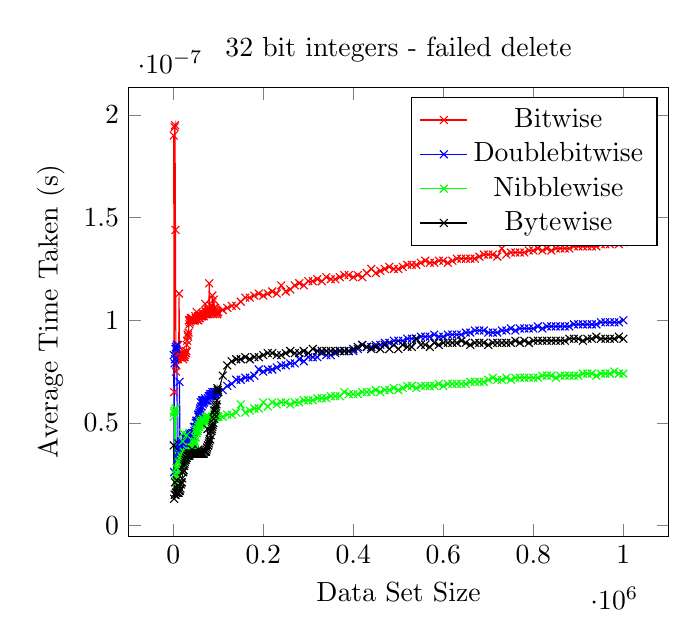
\begin{tikzpicture}
\begin{axis}[
xlabel=Data Set Size,
ylabel=Average Time Taken (s),
title=32 bit integers - failed delete]
\addplot[color=red,mark=x] coordinates {
    (1000,0.00000019)
    (2000,0.000000065)
    (3000,0.000000194)
    (4000,0.000000195)
    (5000,0.000000144)
    (6000,0.000000075)
    (7000,0.000000078)
    (8000,0.000000081)
    (9000,0.000000082)
    (10000,0.000000081)
    (11000,0.000000088)
    (12000,0.000000083)
    (13000,0.000000113)
    (14000,0.000000082)
    (15000,0.000000082)
    (16000,0.000000082)
    (17000,0.000000082)
    (18000,0.000000084)
    (19000,0.000000082)
    (20000,0.000000082)
    (21000,0.000000084)
    (22000,0.000000081)
    (23000,0.000000083)
    (24000,0.000000082)
    (25000,0.000000082)
    (26000,0.000000083)
    (27000,0.000000084)
    (28000,0.000000084)
    (29000,0.000000085)
    (30000,0.000000088)
    (31000,0.00000009)
    (32000,0.000000093)
    (33000,0.000000092)
    (34000,0.000000094)
    (35000,0.0000001)
    (36000,0.000000098)
    (37000,0.000000099)
    (38000,0.0000001)
    (39000,0.000000101)
    (40000,0.0000001)
    (41000,0.000000101)
    (42000,0.000000101)
    (43000,0.0000001)
    (44000,0.0000001)
    (45000,0.0000001)
    (46000,0.0000001)
    (47000,0.0000001)
    (48000,0.0000001)
    (49000,0.000000102)
    (50000,0.000000101)
    (51000,0.000000101)
    (52000,0.000000104)
    (53000,0.000000101)
    (54000,0.0000001)
    (55000,0.000000102)
    (56000,0.0000001)
    (57000,0.000000102)
    (58000,0.000000101)
    (59000,0.000000101)
    (60000,0.000000102)
    (61000,0.000000102)
    (62000,0.000000102)
    (63000,0.000000102)
    (64000,0.000000102)
    (65000,0.000000103)
    (66000,0.000000102)
    (67000,0.000000103)
    (68000,0.000000102)
    (69000,0.000000103)
    (70000,0.000000103)
    (71000,0.000000108)
    (72000,0.000000104)
    (73000,0.000000103)
    (74000,0.000000104)
    (75000,0.000000103)
    (76000,0.000000104)
    (77000,0.000000104)
    (78000,0.000000105)
    (79000,0.000000104)
    (80000,0.000000118)
    (81000,0.000000104)
    (82000,0.000000105)
    (83000,0.000000104)
    (84000,0.000000107)
    (85000,0.000000104)
    (86000,0.000000104)
    (87000,0.000000112)
    (88000,0.000000103)
    (89000,0.000000104)
    (90000,0.00000011)
    (91000,0.000000106)
    (92000,0.000000103)
    (93000,0.000000106)
    (94000,0.000000105)
    (95000,0.000000105)
    (96000,0.000000104)
    (97000,0.000000103)
    (98000,0.000000103)
    (99000,0.000000104)
    (100000,0.000000104)
    (110000,0.000000105)
    (120000,0.000000106)
    (130000,0.000000107)
    (140000,0.000000107)
    (150000,0.000000109)
    (160000,0.000000111)
    (170000,0.000000111)
    (180000,0.000000112)
    (190000,0.000000113)
    (200000,0.000000112)
    (210000,0.000000113)
    (220000,0.000000114)
    (230000,0.000000113)
    (240000,0.000000117)
    (250000,0.000000114)
    (260000,0.000000115)
    (270000,0.000000117)
    (280000,0.000000118)
    (290000,0.000000117)
    (300000,0.000000119)
    (310000,0.000000119)
    (320000,0.00000012)
    (330000,0.000000119)
    (340000,0.000000121)
    (350000,0.00000012)
    (360000,0.00000012)
    (370000,0.000000121)
    (380000,0.000000122)
    (390000,0.000000122)
    (400000,0.000000121)
    (410000,0.000000122)
    (420000,0.000000121)
    (430000,0.000000123)
    (440000,0.000000125)
    (450000,0.000000123)
    (460000,0.000000124)
    (470000,0.000000125)
    (480000,0.000000126)
    (490000,0.000000125)
    (500000,0.000000125)
    (510000,0.000000126)
    (520000,0.000000127)
    (530000,0.000000127)
    (540000,0.000000127)
    (550000,0.000000128)
    (560000,0.000000129)
    (570000,0.000000128)
    (580000,0.000000128)
    (590000,0.000000129)
    (600000,0.000000129)
    (610000,0.000000128)
    (620000,0.000000129)
    (630000,0.00000013)
    (640000,0.00000013)
    (650000,0.00000013)
    (660000,0.00000013)
    (670000,0.00000013)
    (680000,0.000000131)
    (690000,0.000000132)
    (700000,0.000000132)
    (710000,0.000000132)
    (720000,0.000000131)
    (730000,0.000000135)
    (740000,0.000000132)
    (750000,0.000000133)
    (760000,0.000000133)
    (770000,0.000000133)
    (780000,0.000000133)
    (790000,0.000000134)
    (800000,0.000000134)
    (810000,0.000000135)
    (820000,0.000000134)
    (830000,0.000000135)
    (840000,0.000000134)
    (850000,0.000000135)
    (860000,0.000000135)
    (870000,0.000000135)
    (880000,0.000000135)
    (890000,0.000000136)
    (900000,0.000000136)
    (910000,0.000000136)
    (920000,0.000000136)
    (930000,0.000000136)
    (940000,0.000000136)
    (950000,0.000000137)
    (960000,0.000000137)
    (970000,0.000000137)
    (980000,0.000000138)
    (990000,0.000000137)
    (1000000,0.000000138)
};
\addlegendentry{Bitwise}

\addplot[color=blue,mark=x] coordinates {
    (1000,0.000000083)
    (2000,0.000000026)
    (3000,0.000000079)
    (4000,0.000000081)
    (5000,0.000000086)
    (6000,0.000000087)
    (7000,0.000000086)
    (8000,0.000000088)
    (9000,0.000000032)
    (10000,0.000000033)
    (11000,0.00000004)
    (12000,0.000000035)
    (13000,0.000000036)
    (14000,0.00000007)
    (15000,0.000000037)
    (16000,0.000000037)
    (17000,0.00000004)
    (18000,0.000000041)
    (19000,0.000000039)
    (20000,0.000000039)
    (21000,0.00000004)
    (22000,0.00000004)
    (23000,0.00000004)
    (24000,0.000000043)
    (25000,0.00000004)
    (26000,0.00000004)
    (27000,0.000000042)
    (28000,0.000000041)
    (29000,0.000000043)
    (30000,0.000000042)
    (31000,0.000000043)
    (32000,0.000000042)
    (33000,0.000000042)
    (34000,0.000000043)
    (35000,0.000000043)
    (36000,0.000000044)
    (37000,0.000000045)
    (38000,0.000000043)
    (39000,0.000000044)
    (40000,0.000000044)
    (41000,0.000000044)
    (42000,0.000000045)
    (43000,0.000000044)
    (44000,0.000000045)
    (45000,0.000000045)
    (46000,0.000000048)
    (47000,0.000000046)
    (48000,0.000000048)
    (49000,0.000000048)
    (50000,0.00000005)
    (51000,0.000000051)
    (52000,0.00000005)
    (53000,0.000000051)
    (54000,0.000000051)
    (55000,0.000000054)
    (56000,0.000000053)
    (57000,0.000000054)
    (58000,0.000000055)
    (59000,0.000000056)
    (60000,0.000000057)
    (61000,0.00000006)
    (62000,0.000000058)
    (63000,0.000000058)
    (64000,0.000000061)
    (65000,0.00000006)
    (66000,0.000000059)
    (67000,0.000000061)
    (68000,0.00000006)
    (69000,0.00000006)
    (70000,0.000000061)
    (71000,0.000000062)
    (72000,0.000000061)
    (73000,0.000000061)
    (74000,0.000000061)
    (75000,0.000000061)
    (76000,0.000000061)
    (77000,0.000000062)
    (78000,0.000000062)
    (79000,0.000000063)
    (80000,0.000000063)
    (81000,0.000000063)
    (82000,0.000000064)
    (83000,0.000000063)
    (84000,0.000000063)
    (85000,0.000000064)
    (86000,0.000000064)
    (87000,0.000000065)
    (88000,0.000000063)
    (89000,0.000000064)
    (90000,0.000000064)
    (91000,0.000000065)
    (92000,0.000000064)
    (93000,0.000000065)
    (94000,0.000000064)
    (95000,0.000000064)
    (96000,0.000000065)
    (97000,0.000000065)
    (98000,0.000000065)
    (99000,0.000000065)
    (100000,0.000000065)
    (110000,0.000000066)
    (120000,0.000000068)
    (130000,0.000000069)
    (140000,0.000000071)
    (150000,0.000000071)
    (160000,0.000000072)
    (170000,0.000000072)
    (180000,0.000000073)
    (190000,0.000000076)
    (200000,0.000000075)
    (210000,0.000000076)
    (220000,0.000000076)
    (230000,0.000000077)
    (240000,0.000000078)
    (250000,0.000000078)
    (260000,0.000000079)
    (270000,0.000000079)
    (280000,0.000000081)
    (290000,0.00000008)
    (300000,0.000000082)
    (310000,0.000000082)
    (320000,0.000000082)
    (330000,0.000000084)
    (340000,0.000000083)
    (350000,0.000000083)
    (360000,0.000000084)
    (370000,0.000000085)
    (380000,0.000000085)
    (390000,0.000000085)
    (400000,0.000000085)
    (410000,0.000000086)
    (420000,0.000000088)
    (430000,0.000000087)
    (440000,0.000000087)
    (450000,0.000000088)
    (460000,0.000000088)
    (470000,0.000000089)
    (480000,0.000000089)
    (490000,0.00000009)
    (500000,0.00000009)
    (510000,0.00000009)
    (520000,0.000000091)
    (530000,0.000000091)
    (540000,0.000000091)
    (550000,0.000000092)
    (560000,0.000000092)
    (570000,0.000000092)
    (580000,0.000000093)
    (590000,0.000000092)
    (600000,0.000000092)
    (610000,0.000000093)
    (620000,0.000000093)
    (630000,0.000000093)
    (640000,0.000000093)
    (650000,0.000000094)
    (660000,0.000000094)
    (670000,0.000000095)
    (680000,0.000000095)
    (690000,0.000000095)
    (700000,0.000000094)
    (710000,0.000000094)
    (720000,0.000000094)
    (730000,0.000000095)
    (740000,0.000000095)
    (750000,0.000000096)
    (760000,0.000000095)
    (770000,0.000000096)
    (780000,0.000000096)
    (790000,0.000000096)
    (800000,0.000000096)
    (810000,0.000000097)
    (820000,0.000000096)
    (830000,0.000000097)
    (840000,0.000000097)
    (850000,0.000000097)
    (860000,0.000000097)
    (870000,0.000000097)
    (880000,0.000000097)
    (890000,0.000000098)
    (900000,0.000000098)
    (910000,0.000000098)
    (920000,0.000000098)
    (930000,0.000000098)
    (940000,0.000000098)
    (950000,0.000000099)
    (960000,0.000000099)
    (970000,0.000000099)
    (980000,0.000000099)
    (990000,0.000000099)
    (1000000,0.0000001)
};
\addlegendentry{Doublebitwise}

\addplot[color=green,mark=x] coordinates {
    (1000,0.000000053)
    (2000,0.000000055)
    (3000,0.000000056)
    (4000,0.000000025)
    (5000,0.000000057)
    (6000,0.000000021)
    (7000,0.000000028)
    (8000,0.000000022)
    (9000,0.000000022)
    (10000,0.000000025)
    (11000,0.000000025)
    (12000,0.000000027)
    (13000,0.000000031)
    (14000,0.00000003)
    (15000,0.00000003)
    (16000,0.00000003)
    (17000,0.000000032)
    (18000,0.000000034)
    (19000,0.000000032)
    (20000,0.000000033)
    (21000,0.000000041)
    (22000,0.000000045)
    (23000,0.000000036)
    (24000,0.000000034)
    (25000,0.000000032)
    (26000,0.000000033)
    (27000,0.000000035)
    (28000,0.000000034)
    (29000,0.000000034)
    (30000,0.000000044)
    (31000,0.000000037)
    (32000,0.000000035)
    (33000,0.000000034)
    (34000,0.000000034)
    (35000,0.000000035)
    (36000,0.000000034)
    (37000,0.000000034)
    (38000,0.000000036)
    (39000,0.000000036)
    (40000,0.000000035)
    (41000,0.000000038)
    (42000,0.000000036)
    (43000,0.000000037)
    (44000,0.000000038)
    (45000,0.000000038)
    (46000,0.000000039)
    (47000,0.00000004)
    (48000,0.000000041)
    (49000,0.000000043)
    (50000,0.000000043)
    (51000,0.000000047)
    (52000,0.000000045)
    (53000,0.000000046)
    (54000,0.000000046)
    (55000,0.000000047)
    (56000,0.000000048)
    (57000,0.000000049)
    (58000,0.000000048)
    (59000,0.000000051)
    (60000,0.00000005)
    (61000,0.000000049)
    (62000,0.000000049)
    (63000,0.00000005)
    (64000,0.000000051)
    (65000,0.00000005)
    (66000,0.000000052)
    (67000,0.000000051)
    (68000,0.000000051)
    (69000,0.000000051)
    (70000,0.000000051)
    (71000,0.000000051)
    (72000,0.000000053)
    (73000,0.000000051)
    (74000,0.000000051)
    (75000,0.000000052)
    (76000,0.000000053)
    (77000,0.000000053)
    (78000,0.000000052)
    (79000,0.000000052)
    (80000,0.000000052)
    (81000,0.000000052)
    (82000,0.000000052)
    (83000,0.000000052)
    (84000,0.000000052)
    (85000,0.000000052)
    (86000,0.000000053)
    (87000,0.000000053)
    (88000,0.000000053)
    (89000,0.000000053)
    (90000,0.000000053)
    (91000,0.000000055)
    (92000,0.000000052)
    (93000,0.000000053)
    (94000,0.000000053)
    (95000,0.000000053)
    (96000,0.000000053)
    (97000,0.000000053)
    (98000,0.000000053)
    (99000,0.000000053)
    (100000,0.000000053)
    (110000,0.000000053)
    (120000,0.000000054)
    (130000,0.000000054)
    (140000,0.000000055)
    (150000,0.000000059)
    (160000,0.000000055)
    (170000,0.000000056)
    (180000,0.000000057)
    (190000,0.000000057)
    (200000,0.00000006)
    (210000,0.000000058)
    (220000,0.00000006)
    (230000,0.000000059)
    (240000,0.00000006)
    (250000,0.00000006)
    (260000,0.000000059)
    (270000,0.00000006)
    (280000,0.00000006)
    (290000,0.000000061)
    (300000,0.000000061)
    (310000,0.000000061)
    (320000,0.000000062)
    (330000,0.000000062)
    (340000,0.000000062)
    (350000,0.000000063)
    (360000,0.000000063)
    (370000,0.000000063)
    (380000,0.000000065)
    (390000,0.000000064)
    (400000,0.000000064)
    (410000,0.000000064)
    (420000,0.000000065)
    (430000,0.000000065)
    (440000,0.000000065)
    (450000,0.000000066)
    (460000,0.000000065)
    (470000,0.000000066)
    (480000,0.000000066)
    (490000,0.000000067)
    (500000,0.000000066)
    (510000,0.000000067)
    (520000,0.000000068)
    (530000,0.000000068)
    (540000,0.000000067)
    (550000,0.000000068)
    (560000,0.000000068)
    (570000,0.000000068)
    (580000,0.000000068)
    (590000,0.000000069)
    (600000,0.000000068)
    (610000,0.000000069)
    (620000,0.000000069)
    (630000,0.000000069)
    (640000,0.000000069)
    (650000,0.000000069)
    (660000,0.00000007)
    (670000,0.00000007)
    (680000,0.00000007)
    (690000,0.00000007)
    (700000,0.000000071)
    (710000,0.000000072)
    (720000,0.000000071)
    (730000,0.000000071)
    (740000,0.000000072)
    (750000,0.000000071)
    (760000,0.000000072)
    (770000,0.000000072)
    (780000,0.000000072)
    (790000,0.000000072)
    (800000,0.000000072)
    (810000,0.000000072)
    (820000,0.000000073)
    (830000,0.000000073)
    (840000,0.000000073)
    (850000,0.000000072)
    (860000,0.000000073)
    (870000,0.000000073)
    (880000,0.000000073)
    (890000,0.000000073)
    (900000,0.000000073)
    (910000,0.000000074)
    (920000,0.000000074)
    (930000,0.000000074)
    (940000,0.000000073)
    (950000,0.000000074)
    (960000,0.000000074)
    (970000,0.000000074)
    (980000,0.000000075)
    (990000,0.000000074)
    (1000000,0.000000074)
};
\addlegendentry{Nibblewise}
\addplot[color=black,mark=x] coordinates {
    (1000,0.000000039)
    (2000,0.000000013)
    (3000,0.000000015)
    (4000,0.000000021)
    (5000,0.000000015)
    (6000,0.000000016)
    (7000,0.000000016)
    (8000,0.000000022)
    (9000,0.000000016)
    (10000,0.000000016)
    (11000,0.000000016)
    (12000,0.000000016)
    (13000,0.000000017)
    (14000,0.000000017)
    (15000,0.000000017)
    (16000,0.000000018)
    (17000,0.00000002)
    (18000,0.000000021)
    (19000,0.000000021)
    (20000,0.000000023)
    (21000,0.000000026)
    (22000,0.000000026)
    (23000,0.000000027)
    (24000,0.000000029)
    (25000,0.00000003)
    (26000,0.000000031)
    (27000,0.000000032)
    (28000,0.000000032)
    (29000,0.000000033)
    (30000,0.000000033)
    (31000,0.000000034)
    (32000,0.000000034)
    (33000,0.000000034)
    (34000,0.000000035)
    (35000,0.000000035)
    (36000,0.000000034)
    (37000,0.000000035)
    (38000,0.000000035)
    (39000,0.000000035)
    (40000,0.000000035)
    (41000,0.000000035)
    (42000,0.000000037)
    (43000,0.000000035)
    (44000,0.000000035)
    (45000,0.000000035)
    (46000,0.000000035)
    (47000,0.000000035)
    (48000,0.000000035)
    (49000,0.000000035)
    (50000,0.000000035)
    (51000,0.000000035)
    (52000,0.000000035)
    (53000,0.000000035)
    (54000,0.000000035)
    (55000,0.000000035)
    (56000,0.000000037)
    (57000,0.000000035)
    (58000,0.000000035)
    (59000,0.000000035)
    (60000,0.000000035)
    (61000,0.000000035)
    (62000,0.000000035)
    (63000,0.000000035)
    (64000,0.000000035)
    (65000,0.000000035)
    (66000,0.000000035)
    (67000,0.000000035)
    (68000,0.000000035)
    (69000,0.000000036)
    (70000,0.000000036)
    (71000,0.000000036)
    (72000,0.000000036)
    (73000,0.000000036)
    (74000,0.000000037)
    (75000,0.000000038)
    (76000,0.000000047)
    (77000,0.000000039)
    (78000,0.000000039)
    (79000,0.00000004)
    (80000,0.000000041)
    (81000,0.000000042)
    (82000,0.000000042)
    (83000,0.000000044)
    (84000,0.000000046)
    (85000,0.000000046)
    (86000,0.000000047)
    (87000,0.000000048)
    (88000,0.000000049)
    (89000,0.00000005)
    (90000,0.000000052)
    (91000,0.000000056)
    (92000,0.000000054)
    (93000,0.000000056)
    (94000,0.000000057)
    (95000,0.000000058)
    (96000,0.000000059)
    (97000,0.000000061)
    (98000,0.000000067)
    (99000,0.000000066)
    (100000,0.000000065)
    (110000,0.000000073)
    (120000,0.000000078)
    (130000,0.00000008)
    (140000,0.000000081)
    (150000,0.000000081)
    (160000,0.000000082)
    (170000,0.000000081)
    (180000,0.000000082)
    (190000,0.000000082)
    (200000,0.000000083)
    (210000,0.000000084)
    (220000,0.000000084)
    (230000,0.000000083)
    (240000,0.000000083)
    (250000,0.000000084)
    (260000,0.000000085)
    (270000,0.000000084)
    (280000,0.000000084)
    (290000,0.000000085)
    (300000,0.000000084)
    (310000,0.000000086)
    (320000,0.000000085)
    (330000,0.000000085)
    (340000,0.000000085)
    (350000,0.000000085)
    (360000,0.000000085)
    (370000,0.000000085)
    (380000,0.000000085)
    (390000,0.000000085)
    (400000,0.000000086)
    (410000,0.000000087)
    (420000,0.000000088)
    (430000,0.000000087)
    (440000,0.000000086)
    (450000,0.000000087)
    (460000,0.000000086)
    (470000,0.000000088)
    (480000,0.000000086)
    (490000,0.000000088)
    (500000,0.000000086)
    (510000,0.000000088)
    (520000,0.000000087)
    (530000,0.000000087)
    (540000,0.000000091)
    (550000,0.000000088)
    (560000,0.000000088)
    (570000,0.000000087)
    (580000,0.000000089)
    (590000,0.000000088)
    (600000,0.000000089)
    (610000,0.000000089)
    (620000,0.000000089)
    (630000,0.000000089)
    (640000,0.00000009)
    (650000,0.000000089)
    (660000,0.000000088)
    (670000,0.000000089)
    (680000,0.000000089)
    (690000,0.000000089)
    (700000,0.000000088)
    (710000,0.000000089)
    (720000,0.000000089)
    (730000,0.000000089)
    (740000,0.000000089)
    (750000,0.000000089)
    (760000,0.00000009)
    (770000,0.000000089)
    (780000,0.00000009)
    (790000,0.000000089)
    (800000,0.00000009)
    (810000,0.00000009)
    (820000,0.00000009)
    (830000,0.00000009)
    (840000,0.00000009)
    (850000,0.00000009)
    (860000,0.00000009)
    (870000,0.00000009)
    (880000,0.000000091)
    (890000,0.000000091)
    (900000,0.000000091)
    (910000,0.00000009)
    (920000,0.000000091)
    (930000,0.000000091)
    (940000,0.000000092)
    (950000,0.000000091)
    (960000,0.000000091)
    (970000,0.000000091)
    (980000,0.000000091)
    (990000,0.000000092)
    (1000000,0.000000091)
};
\addlegendentry{Bytewise}

\end{axis}
\end{tikzpicture}

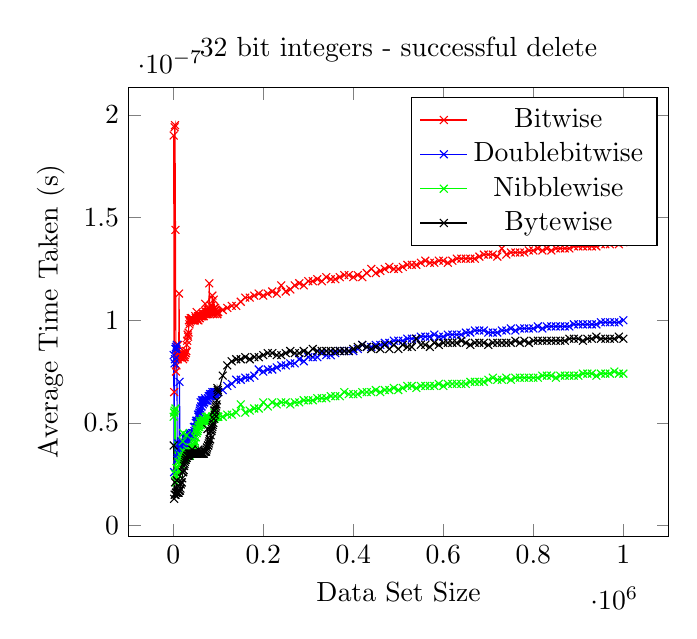
\begin{tikzpicture}
\begin{axis}[
xlabel=Data Set Size,
ylabel=Average Time Taken (s),
title=32 bit integers - successful delete]
\addplot[color=red,mark=x] coordinates {
(1000,0.00000019)
(2000,0.000000065)
(3000,0.000000194)
(4000,0.000000195)
(5000,0.000000144)
(6000,0.000000075)
(7000,0.000000078)
(8000,0.000000081)
(9000,0.000000082)
(10000,0.000000081)
(11000,0.000000088)
(12000,0.000000083)
(13000,0.000000113)
(14000,0.000000082)
(15000,0.000000082)
(16000,0.000000082)
(17000,0.000000082)
(18000,0.000000084)
(19000,0.000000082)
(20000,0.000000082)
(21000,0.000000084)
(22000,0.000000081)
(23000,0.000000083)
(24000,0.000000082)
(25000,0.000000082)
(26000,0.000000083)
(27000,0.000000084)
(28000,0.000000084)
(29000,0.000000085)
(30000,0.000000088)
(31000,0.00000009)
(32000,0.000000093)
(33000,0.000000092)
(34000,0.000000094)
(35000,0.0000001)
(36000,0.000000098)
(37000,0.000000099)
(38000,0.0000001)
(39000,0.000000101)
(40000,0.0000001)
(41000,0.000000101)
(42000,0.000000101)
(43000,0.0000001)
(44000,0.0000001)
(45000,0.0000001)
(46000,0.0000001)
(47000,0.0000001)
(48000,0.0000001)
(49000,0.000000102)
(50000,0.000000101)
(51000,0.000000101)
(52000,0.000000104)
(53000,0.000000101)
(54000,0.0000001)
(55000,0.000000102)
(56000,0.0000001)
(57000,0.000000102)
(58000,0.000000101)
(59000,0.000000101)
(60000,0.000000102)
(61000,0.000000102)
(62000,0.000000102)
(63000,0.000000102)
(64000,0.000000102)
(65000,0.000000103)
(66000,0.000000102)
(67000,0.000000103)
(68000,0.000000102)
(69000,0.000000103)
(70000,0.000000103)
(71000,0.000000108)
(72000,0.000000104)
(73000,0.000000103)
(74000,0.000000104)
(75000,0.000000103)
(76000,0.000000104)
(77000,0.000000104)
(78000,0.000000105)
(79000,0.000000104)
(80000,0.000000118)
(81000,0.000000104)
(82000,0.000000105)
(83000,0.000000104)
(84000,0.000000107)
(85000,0.000000104)
(86000,0.000000104)
(87000,0.000000112)
(88000,0.000000103)
(89000,0.000000104)
(90000,0.00000011)
(91000,0.000000106)
(92000,0.000000103)
(93000,0.000000106)
(94000,0.000000105)
(95000,0.000000105)
(96000,0.000000104)
(97000,0.000000103)
(98000,0.000000103)
(99000,0.000000104)
(100000,0.000000104)
(110000,0.000000105)
(120000,0.000000106)
(130000,0.000000107)
(140000,0.000000107)
(150000,0.000000109)
(160000,0.000000111)
(170000,0.000000111)
(180000,0.000000112)
(190000,0.000000113)
(200000,0.000000112)
(210000,0.000000113)
(220000,0.000000114)
(230000,0.000000113)
(240000,0.000000117)
(250000,0.000000114)
(260000,0.000000115)
(270000,0.000000117)
(280000,0.000000118)
(290000,0.000000117)
(300000,0.000000119)
(310000,0.000000119)
(320000,0.00000012)
(330000,0.000000119)
(340000,0.000000121)
(350000,0.00000012)
(360000,0.00000012)
(370000,0.000000121)
(380000,0.000000122)
(390000,0.000000122)
(400000,0.000000121)
(410000,0.000000122)
(420000,0.000000121)
(430000,0.000000123)
(440000,0.000000125)
(450000,0.000000123)
(460000,0.000000124)
(470000,0.000000125)
(480000,0.000000126)
(490000,0.000000125)
(500000,0.000000125)
(510000,0.000000126)
(520000,0.000000127)
(530000,0.000000127)
(540000,0.000000127)
(550000,0.000000128)
(560000,0.000000129)
(570000,0.000000128)
(580000,0.000000128)
(590000,0.000000129)
(600000,0.000000129)
(610000,0.000000128)
(620000,0.000000129)
(630000,0.00000013)
(640000,0.00000013)
(650000,0.00000013)
(660000,0.00000013)
(670000,0.00000013)
(680000,0.000000131)
(690000,0.000000132)
(700000,0.000000132)
(710000,0.000000132)
(720000,0.000000131)
(730000,0.000000135)
(740000,0.000000132)
(750000,0.000000133)
(760000,0.000000133)
(770000,0.000000133)
(780000,0.000000133)
(790000,0.000000134)
(800000,0.000000134)
(810000,0.000000135)
(820000,0.000000134)
(830000,0.000000135)
(840000,0.000000134)
(850000,0.000000135)
(860000,0.000000135)
(870000,0.000000135)
(880000,0.000000135)
(890000,0.000000136)
(900000,0.000000136)
(910000,0.000000136)
(920000,0.000000136)
(930000,0.000000136)
(940000,0.000000136)
(950000,0.000000137)
(960000,0.000000137)
(970000,0.000000137)
(980000,0.000000138)
(990000,0.000000137)
(1000000,0.000000138)
};
\addlegendentry{Bitwise}
\addplot[color=blue,mark=x] coordinates {
(1000,0.000000083)
(2000,0.000000026)
(3000,0.000000079)
(4000,0.000000081)
(5000,0.000000086)
(6000,0.000000087)
(7000,0.000000086)
(8000,0.000000088)
(9000,0.000000032)
(10000,0.000000033)
(11000,0.00000004)
(12000,0.000000035)
(13000,0.000000036)
(14000,0.00000007)
(15000,0.000000037)
(16000,0.000000037)
(17000,0.00000004)
(18000,0.000000041)
(19000,0.000000039)
(20000,0.000000039)
(21000,0.00000004)
(22000,0.00000004)
(23000,0.00000004)
(24000,0.000000043)
(25000,0.00000004)
(26000,0.00000004)
(27000,0.000000042)
(28000,0.000000041)
(29000,0.000000043)
(30000,0.000000042)
(31000,0.000000043)
(32000,0.000000042)
(33000,0.000000042)
(34000,0.000000043)
(35000,0.000000043)
(36000,0.000000044)
(37000,0.000000045)
(38000,0.000000043)
(39000,0.000000044)
(40000,0.000000044)
(41000,0.000000044)
(42000,0.000000045)
(43000,0.000000044)
(44000,0.000000045)
(45000,0.000000045)
(46000,0.000000048)
(47000,0.000000046)
(48000,0.000000048)
(49000,0.000000048)
(50000,0.00000005)
(51000,0.000000051)
(52000,0.00000005)
(53000,0.000000051)
(54000,0.000000051)
(55000,0.000000054)
(56000,0.000000053)
(57000,0.000000054)
(58000,0.000000055)
(59000,0.000000056)
(60000,0.000000057)
(61000,0.00000006)
(62000,0.000000058)
(63000,0.000000058)
(64000,0.000000061)
(65000,0.00000006)
(66000,0.000000059)
(67000,0.000000061)
(68000,0.00000006)
(69000,0.00000006)
(70000,0.000000061)
(71000,0.000000062)
(72000,0.000000061)
(73000,0.000000061)
(74000,0.000000061)
(75000,0.000000061)
(76000,0.000000061)
(77000,0.000000062)
(78000,0.000000062)
(79000,0.000000063)
(80000,0.000000063)
(81000,0.000000063)
(82000,0.000000064)
(83000,0.000000063)
(84000,0.000000063)
(85000,0.000000064)
(86000,0.000000064)
(87000,0.000000065)
(88000,0.000000063)
(89000,0.000000064)
(90000,0.000000064)
(91000,0.000000065)
(92000,0.000000064)
(93000,0.000000065)
(94000,0.000000064)
(95000,0.000000064)
(96000,0.000000065)
(97000,0.000000065)
(98000,0.000000065)
(99000,0.000000065)
(100000,0.000000065)
(110000,0.000000066)
(120000,0.000000068)
(130000,0.000000069)
(140000,0.000000071)
(150000,0.000000071)
(160000,0.000000072)
(170000,0.000000072)
(180000,0.000000073)
(190000,0.000000076)
(200000,0.000000075)
(210000,0.000000076)
(220000,0.000000076)
(230000,0.000000077)
(240000,0.000000078)
(250000,0.000000078)
(260000,0.000000079)
(270000,0.000000079)
(280000,0.000000081)
(290000,0.00000008)
(300000,0.000000082)
(310000,0.000000082)
(320000,0.000000082)
(330000,0.000000084)
(340000,0.000000083)
(350000,0.000000083)
(360000,0.000000084)
(370000,0.000000085)
(380000,0.000000085)
(390000,0.000000085)
(400000,0.000000085)
(410000,0.000000086)
(420000,0.000000088)
(430000,0.000000087)
(440000,0.000000087)
(450000,0.000000088)
(460000,0.000000088)
(470000,0.000000089)
(480000,0.000000089)
(490000,0.00000009)
(500000,0.00000009)
(510000,0.00000009)
(520000,0.000000091)
(530000,0.000000091)
(540000,0.000000091)
(550000,0.000000092)
(560000,0.000000092)
(570000,0.000000092)
(580000,0.000000093)
(590000,0.000000092)
(600000,0.000000092)
(610000,0.000000093)
(620000,0.000000093)
(630000,0.000000093)
(640000,0.000000093)
(650000,0.000000094)
(660000,0.000000094)
(670000,0.000000095)
(680000,0.000000095)
(690000,0.000000095)
(700000,0.000000094)
(710000,0.000000094)
(720000,0.000000094)
(730000,0.000000095)
(740000,0.000000095)
(750000,0.000000096)
(760000,0.000000095)
(770000,0.000000096)
(780000,0.000000096)
(790000,0.000000096)
(800000,0.000000096)
(810000,0.000000097)
(820000,0.000000096)
(830000,0.000000097)
(840000,0.000000097)
(850000,0.000000097)
(860000,0.000000097)
(870000,0.000000097)
(880000,0.000000097)
(890000,0.000000098)
(900000,0.000000098)
(910000,0.000000098)
(920000,0.000000098)
(930000,0.000000098)
(940000,0.000000098)
(950000,0.000000099)
(960000,0.000000099)
(970000,0.000000099)
(980000,0.000000099)
(990000,0.000000099)
(1000000,0.0000001)
};
\addlegendentry{Doublebitwise}
\addplot[color=green,mark=x] coordinates {
(1000,0.000000053)
(2000,0.000000055)
(3000,0.000000056)
(4000,0.000000025)
(5000,0.000000057)
(6000,0.000000021)
(7000,0.000000028)
(8000,0.000000022)
(9000,0.000000022)
(10000,0.000000025)
(11000,0.000000025)
(12000,0.000000027)
(13000,0.000000031)
(14000,0.00000003)
(15000,0.00000003)
(16000,0.00000003)
(17000,0.000000032)
(18000,0.000000034)
(19000,0.000000032)
(20000,0.000000033)
(21000,0.000000041)
(22000,0.000000045)
(23000,0.000000036)
(24000,0.000000034)
(25000,0.000000032)
(26000,0.000000033)
(27000,0.000000035)
(28000,0.000000034)
(29000,0.000000034)
(30000,0.000000044)
(31000,0.000000037)
(32000,0.000000035)
(33000,0.000000034)
(34000,0.000000034)
(35000,0.000000035)
(36000,0.000000034)
(37000,0.000000034)
(38000,0.000000036)
(39000,0.000000036)
(40000,0.000000035)
(41000,0.000000038)
(42000,0.000000036)
(43000,0.000000037)
(44000,0.000000038)
(45000,0.000000038)
(46000,0.000000039)
(47000,0.00000004)
(48000,0.000000041)
(49000,0.000000043)
(50000,0.000000043)
(51000,0.000000047)
(52000,0.000000045)
(53000,0.000000046)
(54000,0.000000046)
(55000,0.000000047)
(56000,0.000000048)
(57000,0.000000049)
(58000,0.000000048)
(59000,0.000000051)
(60000,0.00000005)
(61000,0.000000049)
(62000,0.000000049)
(63000,0.00000005)
(64000,0.000000051)
(65000,0.00000005)
(66000,0.000000052)
(67000,0.000000051)
(68000,0.000000051)
(69000,0.000000051)
(70000,0.000000051)
(71000,0.000000051)
(72000,0.000000053)
(73000,0.000000051)
(74000,0.000000051)
(75000,0.000000052)
(76000,0.000000053)
(77000,0.000000053)
(78000,0.000000052)
(79000,0.000000052)
(80000,0.000000052)
(81000,0.000000052)
(82000,0.000000052)
(83000,0.000000052)
(84000,0.000000052)
(85000,0.000000052)
(86000,0.000000053)
(87000,0.000000053)
(88000,0.000000053)
(89000,0.000000053)
(90000,0.000000053)
(91000,0.000000055)
(92000,0.000000052)
(93000,0.000000053)
(94000,0.000000053)
(95000,0.000000053)
(96000,0.000000053)
(97000,0.000000053)
(98000,0.000000053)
(99000,0.000000053)
(100000,0.000000053)
(110000,0.000000053)
(120000,0.000000054)
(130000,0.000000054)
(140000,0.000000055)
(150000,0.000000059)
(160000,0.000000055)
(170000,0.000000056)
(180000,0.000000057)
(190000,0.000000057)
(200000,0.00000006)
(210000,0.000000058)
(220000,0.00000006)
(230000,0.000000059)
(240000,0.00000006)
(250000,0.00000006)
(260000,0.000000059)
(270000,0.00000006)
(280000,0.00000006)
(290000,0.000000061)
(300000,0.000000061)
(310000,0.000000061)
(320000,0.000000062)
(330000,0.000000062)
(340000,0.000000062)
(350000,0.000000063)
(360000,0.000000063)
(370000,0.000000063)
(380000,0.000000065)
(390000,0.000000064)
(400000,0.000000064)
(410000,0.000000064)
(420000,0.000000065)
(430000,0.000000065)
(440000,0.000000065)
(450000,0.000000066)
(460000,0.000000065)
(470000,0.000000066)
(480000,0.000000066)
(490000,0.000000067)
(500000,0.000000066)
(510000,0.000000067)
(520000,0.000000068)
(530000,0.000000068)
(540000,0.000000067)
(550000,0.000000068)
(560000,0.000000068)
(570000,0.000000068)
(580000,0.000000068)
(590000,0.000000069)
(600000,0.000000068)
(610000,0.000000069)
(620000,0.000000069)
(630000,0.000000069)
(640000,0.000000069)
(650000,0.000000069)
(660000,0.00000007)
(670000,0.00000007)
(680000,0.00000007)
(690000,0.00000007)
(700000,0.000000071)
(710000,0.000000072)
(720000,0.000000071)
(730000,0.000000071)
(740000,0.000000072)
(750000,0.000000071)
(760000,0.000000072)
(770000,0.000000072)
(780000,0.000000072)
(790000,0.000000072)
(800000,0.000000072)
(810000,0.000000072)
(820000,0.000000073)
(830000,0.000000073)
(840000,0.000000073)
(850000,0.000000072)
(860000,0.000000073)
(870000,0.000000073)
(880000,0.000000073)
(890000,0.000000073)
(900000,0.000000073)
(910000,0.000000074)
(920000,0.000000074)
(930000,0.000000074)
(940000,0.000000073)
(950000,0.000000074)
(960000,0.000000074)
(970000,0.000000074)
(980000,0.000000075)
(990000,0.000000074)
(1000000,0.000000074)
};
\addlegendentry{Nibblewise}
\addplot[color=black,mark=x] coordinates {
(1000,0.000000039)
(2000,0.000000013)
(3000,0.000000015)
(4000,0.000000021)
(5000,0.000000015)
(6000,0.000000016)
(7000,0.000000016)
(8000,0.000000022)
(9000,0.000000016)
(10000,0.000000016)
(11000,0.000000016)
(12000,0.000000016)
(13000,0.000000017)
(14000,0.000000017)
(15000,0.000000017)
(16000,0.000000018)
(17000,0.00000002)
(18000,0.000000021)
(19000,0.000000021)
(20000,0.000000023)
(21000,0.000000026)
(22000,0.000000026)
(23000,0.000000027)
(24000,0.000000029)
(25000,0.00000003)
(26000,0.000000031)
(27000,0.000000032)
(28000,0.000000032)
(29000,0.000000033)
(30000,0.000000033)
(31000,0.000000034)
(32000,0.000000034)
(33000,0.000000034)
(34000,0.000000035)
(35000,0.000000035)
(36000,0.000000034)
(37000,0.000000035)
(38000,0.000000035)
(39000,0.000000035)
(40000,0.000000035)
(41000,0.000000035)
(42000,0.000000037)
(43000,0.000000035)
(44000,0.000000035)
(45000,0.000000035)
(46000,0.000000035)
(47000,0.000000035)
(48000,0.000000035)
(49000,0.000000035)
(50000,0.000000035)
(51000,0.000000035)
(52000,0.000000035)
(53000,0.000000035)
(54000,0.000000035)
(55000,0.000000035)
(56000,0.000000037)
(57000,0.000000035)
(58000,0.000000035)
(59000,0.000000035)
(60000,0.000000035)
(61000,0.000000035)
(62000,0.000000035)
(63000,0.000000035)
(64000,0.000000035)
(65000,0.000000035)
(66000,0.000000035)
(67000,0.000000035)
(68000,0.000000035)
(69000,0.000000036)
(70000,0.000000036)
(71000,0.000000036)
(72000,0.000000036)
(73000,0.000000036)
(74000,0.000000037)
(75000,0.000000038)
(76000,0.000000047)
(77000,0.000000039)
(78000,0.000000039)
(79000,0.00000004)
(80000,0.000000041)
(81000,0.000000042)
(82000,0.000000042)
(83000,0.000000044)
(84000,0.000000046)
(85000,0.000000046)
(86000,0.000000047)
(87000,0.000000048)
(88000,0.000000049)
(89000,0.00000005)
(90000,0.000000052)
(91000,0.000000056)
(92000,0.000000054)
(93000,0.000000056)
(94000,0.000000057)
(95000,0.000000058)
(96000,0.000000059)
(97000,0.000000061)
(98000,0.000000067)
(99000,0.000000066)
(100000,0.000000065)
(110000,0.000000073)
(120000,0.000000078)
(130000,0.00000008)
(140000,0.000000081)
(150000,0.000000081)
(160000,0.000000082)
(170000,0.000000081)
(180000,0.000000082)
(190000,0.000000082)
(200000,0.000000083)
(210000,0.000000084)
(220000,0.000000084)
(230000,0.000000083)
(240000,0.000000083)
(250000,0.000000084)
(260000,0.000000085)
(270000,0.000000084)
(280000,0.000000084)
(290000,0.000000085)
(300000,0.000000084)
(310000,0.000000086)
(320000,0.000000085)
(330000,0.000000085)
(340000,0.000000085)
(350000,0.000000085)
(360000,0.000000085)
(370000,0.000000085)
(380000,0.000000085)
(390000,0.000000085)
(400000,0.000000086)
(410000,0.000000087)
(420000,0.000000088)
(430000,0.000000087)
(440000,0.000000086)
(450000,0.000000087)
(460000,0.000000086)
(470000,0.000000088)
(480000,0.000000086)
(490000,0.000000088)
(500000,0.000000086)
(510000,0.000000088)
(520000,0.000000087)
(530000,0.000000087)
(540000,0.000000091)
(550000,0.000000088)
(560000,0.000000088)
(570000,0.000000087)
(580000,0.000000089)
(590000,0.000000088)
(600000,0.000000089)
(610000,0.000000089)
(620000,0.000000089)
(630000,0.000000089)
(640000,0.00000009)
(650000,0.000000089)
(660000,0.000000088)
(670000,0.000000089)
(680000,0.000000089)
(690000,0.000000089)
(700000,0.000000088)
(710000,0.000000089)
(720000,0.000000089)
(730000,0.000000089)
(740000,0.000000089)
(750000,0.000000089)
(760000,0.00000009)
(770000,0.000000089)
(780000,0.00000009)
(790000,0.000000089)
(800000,0.00000009)
(810000,0.00000009)
(820000,0.00000009)
(830000,0.00000009)
(840000,0.00000009)
(850000,0.00000009)
(860000,0.00000009)
(870000,0.00000009)
(880000,0.000000091)
(890000,0.000000091)
(900000,0.000000091)
(910000,0.00000009)
(920000,0.000000091)
(930000,0.000000091)
(940000,0.000000092)
(950000,0.000000091)
(960000,0.000000091)
(970000,0.000000091)
(980000,0.000000091)
(990000,0.000000092)
(1000000,0.000000091)
};
\addlegendentry{Bytewise}
\end{axis}
\end{tikzpicture}

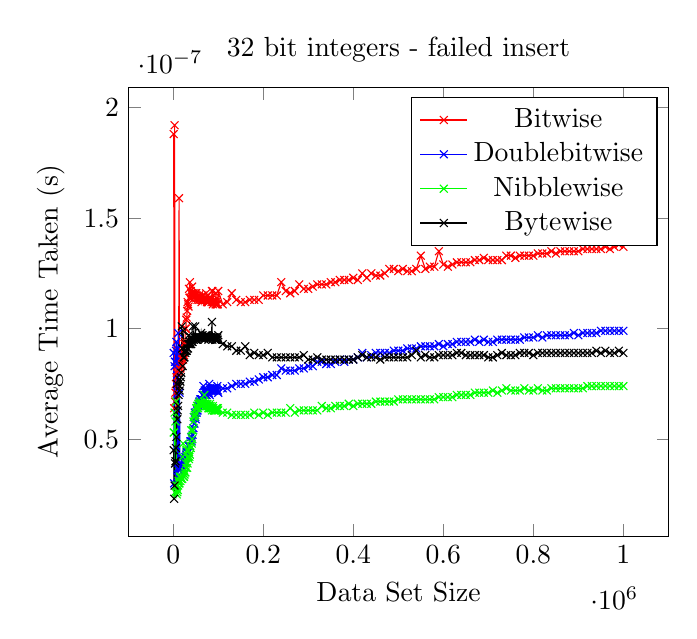
\begin{tikzpicture}
\begin{axis}[
xlabel=Data Set Size,
ylabel=Average Time Taken (s),
title=32 bit integers - failed insert]
\addplot[color=red,mark=x] coordinates {
(1000,0.000000188)
(2000,0.000000064)
(3000,0.000000192)
(4000,0.000000067)
(5000,0.000000071)
(6000,0.000000075)
(7000,0.000000078)
(8000,0.00000008)
(9000,0.000000083)
(10000,0.000000081)
(11000,0.000000081)
(12000,0.000000081)
(13000,0.000000159)
(14000,0.000000082)
(15000,0.000000082)
(16000,0.000000082)
(17000,0.000000083)
(18000,0.000000084)
(19000,0.000000086)
(20000,0.000000087)
(21000,0.000000088)
(22000,0.000000086)
(23000,0.000000089)
(24000,0.000000088)
(25000,0.000000093)
(26000,0.000000094)
(27000,0.0000001)
(28000,0.0000001)
(29000,0.000000104)
(30000,0.000000105)
(31000,0.000000108)
(32000,0.000000112)
(33000,0.000000111)
(34000,0.00000011)
(35000,0.000000118)
(36000,0.000000114)
(37000,0.000000121)
(38000,0.000000114)
(39000,0.000000117)
(40000,0.000000116)
(41000,0.000000116)
(42000,0.000000119)
(43000,0.000000115)
(44000,0.000000115)
(45000,0.000000116)
(46000,0.000000115)
(47000,0.000000114)
(48000,0.000000115)
(49000,0.000000116)
(50000,0.000000115)
(51000,0.000000116)
(52000,0.000000114)
(53000,0.000000115)
(54000,0.000000113)
(55000,0.000000114)
(56000,0.000000114)
(57000,0.000000115)
(58000,0.000000113)
(59000,0.000000114)
(60000,0.000000114)
(61000,0.000000113)
(62000,0.000000114)
(63000,0.000000112)
(64000,0.000000113)
(65000,0.000000115)
(66000,0.000000113)
(67000,0.000000113)
(68000,0.000000113)
(69000,0.000000113)
(70000,0.000000113)
(71000,0.000000113)
(72000,0.000000114)
(73000,0.000000116)
(74000,0.000000113)
(75000,0.000000112)
(76000,0.000000113)
(77000,0.000000112)
(78000,0.000000112)
(79000,0.000000113)
(80000,0.000000113)
(81000,0.000000113)
(82000,0.000000113)
(83000,0.000000114)
(84000,0.000000113)
(85000,0.000000112)
(86000,0.000000117)
(87000,0.000000117)
(88000,0.000000111)
(89000,0.000000112)
(90000,0.000000112)
(91000,0.000000112)
(92000,0.000000112)
(93000,0.000000113)
(94000,0.000000111)
(95000,0.000000116)
(96000,0.000000112)
(97000,0.000000111)
(98000,0.000000111)
(99000,0.000000111)
(100000,0.000000117)
(110000,0.000000111)
(120000,0.000000112)
(130000,0.000000116)
(140000,0.000000113)
(150000,0.000000112)
(160000,0.000000112)
(170000,0.000000113)
(180000,0.000000113)
(190000,0.000000113)
(200000,0.000000115)
(210000,0.000000115)
(220000,0.000000115)
(230000,0.000000115)
(240000,0.000000121)
(250000,0.000000117)
(260000,0.000000116)
(270000,0.000000117)
(280000,0.00000012)
(290000,0.000000118)
(300000,0.000000118)
(310000,0.000000119)
(320000,0.00000012)
(330000,0.00000012)
(340000,0.00000012)
(350000,0.000000121)
(360000,0.000000121)
(370000,0.000000122)
(380000,0.000000122)
(390000,0.000000122)
(400000,0.000000123)
(410000,0.000000122)
(420000,0.000000125)
(430000,0.000000123)
(440000,0.000000125)
(450000,0.000000124)
(460000,0.000000124)
(470000,0.000000125)
(480000,0.000000127)
(490000,0.000000127)
(500000,0.000000126)
(510000,0.000000127)
(520000,0.000000126)
(530000,0.000000126)
(540000,0.000000127)
(550000,0.000000133)
(560000,0.000000127)
(570000,0.000000128)
(580000,0.000000128)
(590000,0.000000135)
(600000,0.000000129)
(610000,0.000000128)
(620000,0.000000129)
(630000,0.00000013)
(640000,0.00000013)
(650000,0.00000013)
(660000,0.00000013)
(670000,0.000000131)
(680000,0.000000131)
(690000,0.000000132)
(700000,0.000000131)
(710000,0.000000131)
(720000,0.000000131)
(730000,0.000000131)
(740000,0.000000133)
(750000,0.000000133)
(760000,0.000000132)
(770000,0.000000133)
(780000,0.000000133)
(790000,0.000000133)
(800000,0.000000133)
(810000,0.000000134)
(820000,0.000000134)
(830000,0.000000134)
(840000,0.000000135)
(850000,0.000000134)
(860000,0.000000135)
(870000,0.000000135)
(880000,0.000000135)
(890000,0.000000135)
(900000,0.000000135)
(910000,0.000000136)
(920000,0.000000136)
(930000,0.000000136)
(940000,0.000000136)
(950000,0.000000136)
(960000,0.000000137)
(970000,0.000000136)
(980000,0.000000137)
(990000,0.000000138)
(1000000,0.000000137)
};
\addlegendentry{Bitwise}
\addplot[color=blue,mark=x] coordinates {
(1000,0.000000089)
(2000,0.00000003)
(3000,0.000000083)
(4000,0.000000085)
(5000,0.000000085)
(6000,0.00000009)
(7000,0.000000094)
(8000,0.000000091)
(9000,0.000000033)
(10000,0.000000037)
(11000,0.000000098)
(12000,0.000000036)
(13000,0.000000037)
(14000,0.000000071)
(15000,0.000000037)
(16000,0.000000039)
(17000,0.000000038)
(18000,0.000000039)
(19000,0.000000038)
(20000,0.000000042)
(21000,0.000000042)
(22000,0.00000004)
(23000,0.00000004)
(24000,0.000000041)
(25000,0.000000041)
(26000,0.000000041)
(27000,0.000000042)
(28000,0.000000042)
(29000,0.000000043)
(30000,0.000000044)
(31000,0.000000044)
(32000,0.000000044)
(33000,0.000000044)
(34000,0.000000047)
(35000,0.000000047)
(36000,0.000000047)
(37000,0.000000047)
(38000,0.000000049)
(39000,0.000000049)
(40000,0.000000051)
(41000,0.000000049)
(42000,0.00000005)
(43000,0.000000052)
(44000,0.000000054)
(45000,0.000000055)
(46000,0.00000006)
(47000,0.000000057)
(48000,0.000000062)
(49000,0.00000006)
(50000,0.000000059)
(51000,0.000000062)
(52000,0.000000062)
(53000,0.000000063)
(54000,0.000000063)
(55000,0.000000065)
(56000,0.000000065)
(57000,0.000000066)
(58000,0.000000067)
(59000,0.000000067)
(60000,0.000000068)
(61000,0.000000068)
(62000,0.000000068)
(63000,0.000000068)
(64000,0.000000068)
(65000,0.00000007)
(66000,0.00000007)
(67000,0.000000074)
(68000,0.00000007)
(69000,0.00000007)
(70000,0.000000072)
(71000,0.000000071)
(72000,0.00000007)
(73000,0.000000072)
(74000,0.00000007)
(75000,0.000000071)
(76000,0.000000072)
(77000,0.000000071)
(78000,0.000000072)
(79000,0.000000071)
(80000,0.000000075)
(81000,0.00000007)
(82000,0.000000073)
(83000,0.000000072)
(84000,0.000000072)
(85000,0.000000073)
(86000,0.000000072)
(87000,0.000000072)
(88000,0.000000073)
(89000,0.000000072)
(90000,0.000000072)
(91000,0.000000073)
(92000,0.000000072)
(93000,0.000000073)
(94000,0.000000072)
(95000,0.000000072)
(96000,0.000000073)
(97000,0.000000072)
(98000,0.000000074)
(99000,0.000000072)
(100000,0.000000071)
(110000,0.000000073)
(120000,0.000000073)
(130000,0.000000074)
(140000,0.000000075)
(150000,0.000000075)
(160000,0.000000075)
(170000,0.000000076)
(180000,0.000000076)
(190000,0.000000077)
(200000,0.000000078)
(210000,0.000000078)
(220000,0.000000079)
(230000,0.000000079)
(240000,0.000000082)
(250000,0.000000081)
(260000,0.000000081)
(270000,0.000000081)
(280000,0.000000082)
(290000,0.000000082)
(300000,0.000000083)
(310000,0.000000083)
(320000,0.000000085)
(330000,0.000000085)
(340000,0.000000084)
(350000,0.000000084)
(360000,0.000000085)
(370000,0.000000086)
(380000,0.000000085)
(390000,0.000000086)
(400000,0.000000086)
(410000,0.000000087)
(420000,0.000000089)
(430000,0.000000087)
(440000,0.000000088)
(450000,0.000000089)
(460000,0.000000089)
(470000,0.000000089)
(480000,0.000000089)
(490000,0.00000009)
(500000,0.00000009)
(510000,0.00000009)
(520000,0.000000091)
(530000,0.000000091)
(540000,0.000000091)
(550000,0.000000092)
(560000,0.000000092)
(570000,0.000000092)
(580000,0.000000092)
(590000,0.000000093)
(600000,0.000000092)
(610000,0.000000093)
(620000,0.000000093)
(630000,0.000000094)
(640000,0.000000094)
(650000,0.000000094)
(660000,0.000000094)
(670000,0.000000095)
(680000,0.000000094)
(690000,0.000000095)
(700000,0.000000094)
(710000,0.000000094)
(720000,0.000000095)
(730000,0.000000095)
(740000,0.000000095)
(750000,0.000000095)
(760000,0.000000095)
(770000,0.000000095)
(780000,0.000000096)
(790000,0.000000096)
(800000,0.000000096)
(810000,0.000000097)
(820000,0.000000096)
(830000,0.000000097)
(840000,0.000000097)
(850000,0.000000097)
(860000,0.000000097)
(870000,0.000000097)
(880000,0.000000097)
(890000,0.000000098)
(900000,0.000000097)
(910000,0.000000098)
(920000,0.000000098)
(930000,0.000000098)
(940000,0.000000098)
(950000,0.000000099)
(960000,0.000000099)
(970000,0.000000099)
(980000,0.000000099)
(990000,0.000000099)
(1000000,0.000000099)
};
\addlegendentry{Doublebitwise}
\addplot[color=green,mark=x] coordinates {
(1000,0.000000053)
(2000,0.000000053)
(3000,0.000000062)
(4000,0.000000026)
(5000,0.000000058)
(6000,0.000000067)
(7000,0.000000029)
(8000,0.000000025)
(9000,0.000000026)
(10000,0.000000027)
(11000,0.000000029)
(12000,0.000000031)
(13000,0.00000003)
(14000,0.00000003)
(15000,0.000000033)
(16000,0.000000031)
(17000,0.000000033)
(18000,0.000000032)
(19000,0.000000032)
(20000,0.000000032)
(21000,0.000000042)
(22000,0.000000048)
(23000,0.000000033)
(24000,0.000000033)
(25000,0.000000034)
(26000,0.000000035)
(27000,0.000000035)
(28000,0.000000039)
(29000,0.000000037)
(30000,0.000000045)
(31000,0.000000037)
(32000,0.000000039)
(33000,0.000000042)
(34000,0.000000045)
(35000,0.000000041)
(36000,0.000000042)
(37000,0.000000043)
(38000,0.000000047)
(39000,0.000000046)
(40000,0.000000054)
(41000,0.000000048)
(42000,0.00000005)
(43000,0.000000054)
(44000,0.000000054)
(45000,0.000000058)
(46000,0.00000006)
(47000,0.00000006)
(48000,0.000000061)
(49000,0.000000061)
(50000,0.000000062)
(51000,0.000000064)
(52000,0.000000064)
(53000,0.000000065)
(54000,0.000000065)
(55000,0.000000064)
(56000,0.000000066)
(57000,0.000000066)
(58000,0.000000066)
(59000,0.000000066)
(60000,0.000000067)
(61000,0.000000065)
(62000,0.000000066)
(63000,0.000000065)
(64000,0.000000066)
(65000,0.000000066)
(66000,0.000000066)
(67000,0.000000066)
(68000,0.000000067)
(69000,0.00000007)
(70000,0.000000066)
(71000,0.000000066)
(72000,0.000000066)
(73000,0.000000065)
(74000,0.000000065)
(75000,0.000000065)
(76000,0.000000066)
(77000,0.000000065)
(78000,0.000000064)
(79000,0.000000064)
(80000,0.000000065)
(81000,0.000000064)
(82000,0.000000066)
(83000,0.000000065)
(84000,0.000000064)
(85000,0.000000064)
(86000,0.000000063)
(87000,0.000000064)
(88000,0.000000065)
(89000,0.000000064)
(90000,0.000000063)
(91000,0.000000063)
(92000,0.000000063)
(93000,0.000000063)
(94000,0.000000063)
(95000,0.000000063)
(96000,0.000000064)
(97000,0.000000064)
(98000,0.000000063)
(99000,0.000000064)
(100000,0.000000063)
(110000,0.000000062)
(120000,0.000000062)
(130000,0.000000061)
(140000,0.000000061)
(150000,0.000000061)
(160000,0.000000061)
(170000,0.000000061)
(180000,0.000000062)
(190000,0.000000061)
(200000,0.000000062)
(210000,0.000000061)
(220000,0.000000062)
(230000,0.000000062)
(240000,0.000000062)
(250000,0.000000062)
(260000,0.000000064)
(270000,0.000000062)
(280000,0.000000063)
(290000,0.000000063)
(300000,0.000000063)
(310000,0.000000063)
(320000,0.000000063)
(330000,0.000000065)
(340000,0.000000064)
(350000,0.000000064)
(360000,0.000000065)
(370000,0.000000065)
(380000,0.000000065)
(390000,0.000000066)
(400000,0.000000065)
(410000,0.000000066)
(420000,0.000000066)
(430000,0.000000066)
(440000,0.000000066)
(450000,0.000000067)
(460000,0.000000067)
(470000,0.000000067)
(480000,0.000000067)
(490000,0.000000067)
(500000,0.000000068)
(510000,0.000000068)
(520000,0.000000068)
(530000,0.000000068)
(540000,0.000000068)
(550000,0.000000068)
(560000,0.000000068)
(570000,0.000000068)
(580000,0.000000068)
(590000,0.000000069)
(600000,0.000000069)
(610000,0.000000069)
(620000,0.000000069)
(630000,0.00000007)
(640000,0.00000007)
(650000,0.00000007)
(660000,0.00000007)
(670000,0.000000071)
(680000,0.000000071)
(690000,0.000000071)
(700000,0.000000071)
(710000,0.000000072)
(720000,0.000000071)
(730000,0.000000072)
(740000,0.000000073)
(750000,0.000000072)
(760000,0.000000072)
(770000,0.000000072)
(780000,0.000000073)
(790000,0.000000072)
(800000,0.000000072)
(810000,0.000000073)
(820000,0.000000072)
(830000,0.000000072)
(840000,0.000000073)
(850000,0.000000073)
(860000,0.000000073)
(870000,0.000000073)
(880000,0.000000073)
(890000,0.000000073)
(900000,0.000000073)
(910000,0.000000073)
(920000,0.000000074)
(930000,0.000000074)
(940000,0.000000074)
(950000,0.000000074)
(960000,0.000000074)
(970000,0.000000074)
(980000,0.000000074)
(990000,0.000000074)
(1000000,0.000000074)
};
\addlegendentry{Nibblewise}
\addplot[color=black,mark=x] coordinates {
(1000,0.000000045)
(2000,0.000000023)
(3000,0.000000029)
(4000,0.000000039)
(5000,0.00000004)
(6000,0.000000046)
(7000,0.000000051)
(8000,0.000000075)
(9000,0.000000059)
(10000,0.000000063)
(11000,0.000000065)
(12000,0.00000007)
(13000,0.000000077)
(14000,0.000000072)
(15000,0.000000074)
(16000,0.000000076)
(17000,0.000000078)
(18000,0.00000008)
(19000,0.000000101)
(20000,0.000000091)
(21000,0.000000083)
(22000,0.000000099)
(23000,0.000000087)
(24000,0.000000087)
(25000,0.000000087)
(26000,0.00000009)
(27000,0.000000089)
(28000,0.00000009)
(29000,0.00000009)
(30000,0.00000009)
(31000,0.000000091)
(32000,0.000000093)
(33000,0.000000091)
(34000,0.000000097)
(35000,0.000000093)
(36000,0.000000093)
(37000,0.000000094)
(38000,0.000000093)
(39000,0.000000096)
(40000,0.000000093)
(41000,0.000000094)
(42000,0.000000095)
(43000,0.000000094)
(44000,0.000000101)
(45000,0.000000095)
(46000,0.000000095)
(47000,0.000000096)
(48000,0.000000096)
(49000,0.000000101)
(50000,0.000000095)
(51000,0.000000096)
(52000,0.000000095)
(53000,0.000000095)
(54000,0.000000096)
(55000,0.000000096)
(56000,0.000000096)
(57000,0.000000096)
(58000,0.000000096)
(59000,0.000000096)
(60000,0.000000096)
(61000,0.000000096)
(62000,0.000000098)
(63000,0.000000096)
(64000,0.000000096)
(65000,0.000000097)
(66000,0.000000096)
(67000,0.000000096)
(68000,0.000000096)
(69000,0.000000096)
(70000,0.000000095)
(71000,0.000000096)
(72000,0.000000097)
(73000,0.000000096)
(74000,0.000000097)
(75000,0.000000096)
(76000,0.000000097)
(77000,0.000000096)
(78000,0.000000095)
(79000,0.000000096)
(80000,0.000000096)
(81000,0.000000096)
(82000,0.000000096)
(83000,0.000000096)
(84000,0.000000096)
(85000,0.000000096)
(86000,0.000000103)
(87000,0.000000095)
(88000,0.000000096)
(89000,0.000000096)
(90000,0.000000096)
(91000,0.000000096)
(92000,0.000000096)
(93000,0.000000095)
(94000,0.000000095)
(95000,0.000000095)
(96000,0.000000095)
(97000,0.000000095)
(98000,0.000000096)
(99000,0.000000095)
(100000,0.000000097)
(110000,0.000000093)
(120000,0.000000092)
(130000,0.000000092)
(140000,0.00000009)
(150000,0.00000009)
(160000,0.000000092)
(170000,0.000000088)
(180000,0.000000089)
(190000,0.000000088)
(200000,0.000000088)
(210000,0.000000089)
(220000,0.000000087)
(230000,0.000000087)
(240000,0.000000087)
(250000,0.000000087)
(260000,0.000000087)
(270000,0.000000087)
(280000,0.000000087)
(290000,0.000000088)
(300000,0.000000086)
(310000,0.000000086)
(320000,0.000000087)
(330000,0.000000086)
(340000,0.000000086)
(350000,0.000000086)
(360000,0.000000086)
(370000,0.000000086)
(380000,0.000000086)
(390000,0.000000086)
(400000,0.000000086)
(410000,0.000000087)
(420000,0.000000088)
(430000,0.000000087)
(440000,0.000000087)
(450000,0.000000087)
(460000,0.000000086)
(470000,0.000000087)
(480000,0.000000087)
(490000,0.000000087)
(500000,0.000000087)
(510000,0.000000087)
(520000,0.000000087)
(530000,0.000000088)
(540000,0.00000009)
(550000,0.000000087)
(560000,0.000000088)
(570000,0.000000087)
(580000,0.000000087)
(590000,0.000000088)
(600000,0.000000088)
(610000,0.000000088)
(620000,0.000000088)
(630000,0.000000089)
(640000,0.000000089)
(650000,0.000000088)
(660000,0.000000088)
(670000,0.000000088)
(680000,0.000000088)
(690000,0.000000088)
(700000,0.000000087)
(710000,0.000000087)
(720000,0.000000088)
(730000,0.000000089)
(740000,0.000000088)
(750000,0.000000088)
(760000,0.000000088)
(770000,0.000000089)
(780000,0.000000089)
(790000,0.000000089)
(800000,0.000000088)
(810000,0.000000089)
(820000,0.000000089)
(830000,0.000000089)
(840000,0.000000089)
(850000,0.000000089)
(860000,0.000000089)
(870000,0.000000089)
(880000,0.000000089)
(890000,0.000000089)
(900000,0.000000089)
(910000,0.000000089)
(920000,0.000000089)
(930000,0.000000089)
(940000,0.00000009)
(950000,0.000000089)
(960000,0.00000009)
(970000,0.000000089)
(980000,0.000000089)
(990000,0.00000009)
(1000000,0.000000089)
};
\addlegendentry{Bytewise}
\end{axis}
\end{tikzpicture}

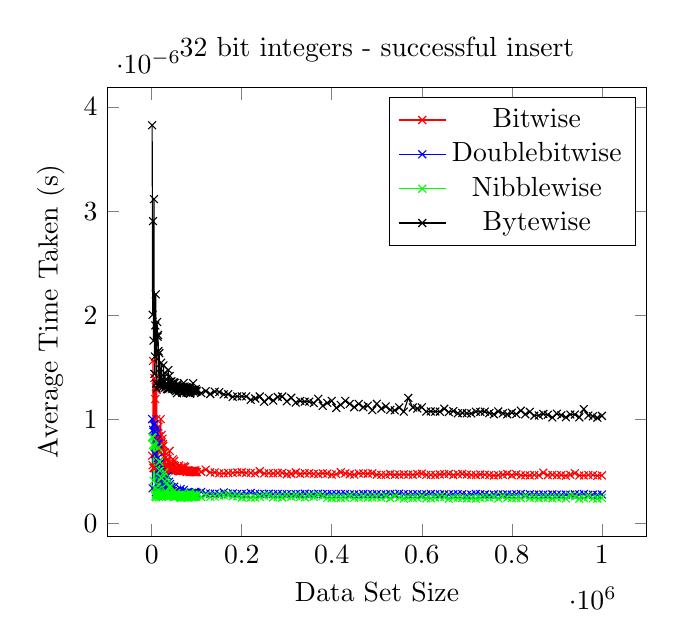
\begin{tikzpicture}
\begin{axis}[
xlabel=Data Set Size,
ylabel=Average Time Taken (s),
title=32 bit integers - successful insert]
\addplot[color=red,mark=x] coordinates {
(1000,0.000000653)
(2000,0.000000561)
(3000,0.000001563)
(4000,0.000000537)
(5000,0.000000533)
(6000,0.000001398)
(7000,0.000000533)
(8000,0.000001196)
(9000,0.000001313)
(10000,0.000001004)
(11000,0.000001284)
(12000,0.000000906)
(13000,0.000000711)
(14000,0.00000081)
(15000,0.000000932)
(16000,0.000000838)
(17000,0.000000751)
(18000,0.000000686)
(19000,0.000000737)
(20000,0.000001004)
(21000,0.000000778)
(22000,0.000000852)
(23000,0.000000736)
(24000,0.000000817)
(25000,0.000000765)
(26000,0.000000746)
(27000,0.000000528)
(28000,0.000000652)
(29000,0.000000685)
(30000,0.000000631)
(31000,0.00000052)
(32000,0.000000548)
(33000,0.000000523)
(34000,0.000000553)
(35000,0.000000619)
(36000,0.000000538)
(37000,0.000000512)
(38000,0.000000553)
(39000,0.000000525)
(40000,0.0000007)
(41000,0.000000571)
(42000,0.000000524)
(43000,0.000000512)
(44000,0.000000507)
(45000,0.000000509)
(46000,0.000000568)
(47000,0.000000619)
(48000,0.00000052)
(49000,0.000000562)
(50000,0.000000604)
(51000,0.00000053)
(52000,0.000000556)
(53000,0.00000051)
(54000,0.000000534)
(55000,0.000000515)
(56000,0.000000533)
(57000,0.000000538)
(58000,0.000000518)
(59000,0.000000532)
(60000,0.000000507)
(61000,0.00000056)
(62000,0.000000501)
(63000,0.000000512)
(64000,0.000000512)
(65000,0.000000509)
(66000,0.000000535)
(67000,0.00000054)
(68000,0.000000509)
(69000,0.000000505)
(70000,0.000000514)
(71000,0.000000508)
(72000,0.000000551)
(73000,0.000000511)
(74000,0.000000544)
(75000,0.00000051)
(76000,0.000000504)
(77000,0.000000505)
(78000,0.000000497)
(79000,0.000000503)
(80000,0.000000512)
(81000,0.000000509)
(82000,0.000000506)
(83000,0.000000507)
(84000,0.000000496)
(85000,0.000000506)
(86000,0.000000496)
(87000,0.000000506)
(88000,0.000000496)
(89000,0.000000504)
(90000,0.000000507)
(91000,0.000000495)
(92000,0.000000507)
(93000,0.00000051)
(94000,0.000000499)
(95000,0.000000493)
(96000,0.0000005)
(97000,0.000000512)
(98000,0.000000495)
(99000,0.000000495)
(100000,0.000000496)
(110000,0.000000499)
(120000,0.00000052)
(130000,0.000000492)
(140000,0.000000492)
(150000,0.000000484)
(160000,0.000000483)
(170000,0.000000487)
(180000,0.000000488)
(190000,0.000000493)
(200000,0.000000494)
(210000,0.000000489)
(220000,0.000000488)
(230000,0.000000484)
(240000,0.000000504)
(250000,0.000000483)
(260000,0.000000486)
(270000,0.000000484)
(280000,0.000000487)
(290000,0.000000489)
(300000,0.000000475)
(310000,0.00000048)
(320000,0.000000492)
(330000,0.000000479)
(340000,0.000000485)
(350000,0.000000485)
(360000,0.000000479)
(370000,0.000000477)
(380000,0.000000483)
(390000,0.000000482)
(400000,0.000000472)
(410000,0.000000476)
(420000,0.000000494)
(430000,0.000000484)
(440000,0.000000475)
(450000,0.000000472)
(460000,0.000000483)
(470000,0.000000483)
(480000,0.00000048)
(490000,0.000000484)
(500000,0.000000471)
(510000,0.000000469)
(520000,0.000000469)
(530000,0.000000477)
(540000,0.00000047)
(550000,0.000000471)
(560000,0.000000475)
(570000,0.000000471)
(580000,0.00000047)
(590000,0.000000478)
(600000,0.000000481)
(610000,0.00000047)
(620000,0.000000469)
(630000,0.000000467)
(640000,0.000000473)
(650000,0.000000476)
(660000,0.000000478)
(670000,0.000000467)
(680000,0.000000475)
(690000,0.000000479)
(700000,0.000000472)
(710000,0.000000468)
(720000,0.000000467)
(730000,0.000000473)
(740000,0.00000047)
(750000,0.000000467)
(760000,0.000000463)
(770000,0.000000466)
(780000,0.000000471)
(790000,0.000000478)
(800000,0.000000466)
(810000,0.000000475)
(820000,0.000000465)
(830000,0.000000465)
(840000,0.000000464)
(850000,0.000000468)
(860000,0.000000465)
(870000,0.00000049)
(880000,0.000000466)
(890000,0.00000047)
(900000,0.000000465)
(910000,0.000000467)
(920000,0.000000461)
(930000,0.000000471)
(940000,0.000000485)
(950000,0.000000463)
(960000,0.000000463)
(970000,0.000000468)
(980000,0.000000468)
(990000,0.00000046)
(1000000,0.000000464)
};
\addlegendentry{Bitwise}
\addplot[color=blue,mark=x] coordinates {
(1000,0.000001004)
(2000,0.00000034)
(3000,0.0000009)
(4000,0.000000949)
(5000,0.000000881)
(6000,0.000000958)
(7000,0.00000067)
(8000,0.000000883)
(9000,0.000000302)
(10000,0.000000795)
(11000,0.00000087)
(12000,0.000000301)
(13000,0.000000769)
(14000,0.000000632)
(15000,0.000000766)
(16000,0.000000521)
(17000,0.000000293)
(18000,0.000000316)
(19000,0.000000579)
(20000,0.000000497)
(21000,0.000000474)
(22000,0.000000426)
(23000,0.000000312)
(24000,0.000000299)
(25000,0.000000384)
(26000,0.000000436)
(27000,0.000000294)
(28000,0.000000295)
(29000,0.000000294)
(30000,0.000000412)
(31000,0.00000031)
(32000,0.000000292)
(33000,0.000000373)
(34000,0.00000029)
(35000,0.000000458)
(36000,0.00000032)
(37000,0.000000291)
(38000,0.00000029)
(39000,0.000000404)
(40000,0.000000339)
(41000,0.000000381)
(42000,0.000000293)
(43000,0.000000353)
(44000,0.00000035)
(45000,0.000000292)
(46000,0.000000303)
(47000,0.00000031)
(48000,0.0000003)
(49000,0.00000029)
(50000,0.000000356)
(51000,0.0000003)
(52000,0.000000297)
(53000,0.000000294)
(54000,0.000000313)
(55000,0.000000309)
(56000,0.000000287)
(57000,0.000000295)
(58000,0.000000289)
(59000,0.000000291)
(60000,0.000000292)
(61000,0.00000029)
(62000,0.000000313)
(63000,0.000000289)
(64000,0.000000333)
(65000,0.000000292)
(66000,0.000000299)
(67000,0.000000289)
(68000,0.000000291)
(69000,0.000000294)
(70000,0.000000291)
(71000,0.000000325)
(72000,0.0000003)
(73000,0.000000288)
(74000,0.000000286)
(75000,0.000000289)
(76000,0.000000289)
(77000,0.000000297)
(78000,0.000000299)
(79000,0.000000295)
(80000,0.000000297)
(81000,0.000000288)
(82000,0.000000288)
(83000,0.000000288)
(84000,0.000000289)
(85000,0.000000293)
(86000,0.000000294)
(87000,0.000000289)
(88000,0.000000287)
(89000,0.000000295)
(90000,0.000000295)
(91000,0.000000291)
(92000,0.000000293)
(93000,0.000000289)
(94000,0.000000288)
(95000,0.000000297)
(96000,0.000000291)
(97000,0.000000306)
(98000,0.000000291)
(99000,0.000000289)
(100000,0.000000296)
(110000,0.000000306)
(120000,0.000000291)
(130000,0.000000289)
(140000,0.000000289)
(150000,0.000000287)
(160000,0.0000003)
(170000,0.000000289)
(180000,0.000000292)
(190000,0.000000287)
(200000,0.000000287)
(210000,0.000000287)
(220000,0.000000296)
(230000,0.000000289)
(240000,0.000000284)
(250000,0.000000287)
(260000,0.000000288)
(270000,0.000000284)
(280000,0.000000287)
(290000,0.000000285)
(300000,0.000000284)
(310000,0.000000284)
(320000,0.000000285)
(330000,0.000000283)
(340000,0.000000288)
(350000,0.000000284)
(360000,0.000000283)
(370000,0.000000289)
(380000,0.000000284)
(390000,0.000000285)
(400000,0.000000285)
(410000,0.000000284)
(420000,0.000000285)
(430000,0.000000286)
(440000,0.000000282)
(450000,0.000000282)
(460000,0.000000281)
(470000,0.000000286)
(480000,0.000000283)
(490000,0.000000283)
(500000,0.000000285)
(510000,0.000000281)
(520000,0.000000281)
(530000,0.000000287)
(540000,0.000000283)
(550000,0.000000289)
(560000,0.000000284)
(570000,0.000000282)
(580000,0.000000283)
(590000,0.000000284)
(600000,0.000000281)
(610000,0.000000281)
(620000,0.000000286)
(630000,0.000000282)
(640000,0.000000281)
(650000,0.000000283)
(660000,0.000000281)
(670000,0.000000282)
(680000,0.000000284)
(690000,0.000000284)
(700000,0.000000275)
(710000,0.00000028)
(720000,0.000000286)
(730000,0.000000284)
(740000,0.000000281)
(750000,0.000000275)
(760000,0.000000282)
(770000,0.000000282)
(780000,0.00000028)
(790000,0.000000281)
(800000,0.00000028)
(810000,0.000000283)
(820000,0.000000286)
(830000,0.000000278)
(840000,0.000000283)
(850000,0.000000279)
(860000,0.00000028)
(870000,0.000000281)
(880000,0.000000277)
(890000,0.000000282)
(900000,0.00000028)
(910000,0.000000278)
(920000,0.00000028)
(930000,0.000000279)
(940000,0.000000282)
(950000,0.000000281)
(960000,0.000000285)
(970000,0.000000278)
(980000,0.000000279)
(990000,0.000000277)
(1000000,0.000000281)
};
\addlegendentry{Doublebitwise}
\addplot[color=green,mark=x] coordinates {
(1000,0.000000832)
(2000,0.000000826)
(3000,0.000000758)
(4000,0.000000414)
(5000,0.000000748)
(6000,0.000000742)
(7000,0.00000034)
(8000,0.000000263)
(9000,0.000000284)
(10000,0.000000253)
(11000,0.000000268)
(12000,0.0000003)
(13000,0.000000281)
(14000,0.000000325)
(15000,0.00000073)
(16000,0.000000256)
(17000,0.000000596)
(18000,0.000000509)
(19000,0.000000275)
(20000,0.00000026)
(21000,0.000000438)
(22000,0.00000044)
(23000,0.000000265)
(24000,0.000000263)
(25000,0.000000278)
(26000,0.000000267)
(27000,0.000000275)
(28000,0.000000494)
(29000,0.000000289)
(30000,0.000000282)
(31000,0.000000293)
(32000,0.00000031)
(33000,0.000000387)
(34000,0.000000429)
(35000,0.000000275)
(36000,0.000000264)
(37000,0.000000288)
(38000,0.000000261)
(39000,0.000000269)
(40000,0.000000347)
(41000,0.000000363)
(42000,0.000000268)
(43000,0.000000271)
(44000,0.000000277)
(45000,0.000000279)
(46000,0.000000266)
(47000,0.000000304)
(48000,0.000000252)
(49000,0.000000269)
(50000,0.000000262)
(51000,0.000000269)
(52000,0.000000273)
(53000,0.000000258)
(54000,0.000000273)
(55000,0.000000296)
(56000,0.000000269)
(57000,0.000000264)
(58000,0.000000266)
(59000,0.000000265)
(60000,0.000000278)
(61000,0.000000273)
(62000,0.000000273)
(63000,0.000000257)
(64000,0.000000259)
(65000,0.000000251)
(66000,0.000000249)
(67000,0.000000286)
(68000,0.000000268)
(69000,0.000000257)
(70000,0.000000263)
(71000,0.000000274)
(72000,0.000000255)
(73000,0.000000252)
(74000,0.000000258)
(75000,0.000000272)
(76000,0.000000266)
(77000,0.000000255)
(78000,0.000000272)
(79000,0.000000254)
(80000,0.000000252)
(81000,0.000000266)
(82000,0.000000272)
(83000,0.000000254)
(84000,0.000000258)
(85000,0.000000297)
(86000,0.00000028)
(87000,0.000000267)
(88000,0.000000258)
(89000,0.000000255)
(90000,0.000000258)
(91000,0.000000259)
(92000,0.000000278)
(93000,0.000000265)
(94000,0.000000278)
(95000,0.000000263)
(96000,0.000000271)
(97000,0.00000026)
(98000,0.000000259)
(99000,0.000000267)
(100000,0.00000028)
(110000,0.000000257)
(120000,0.000000272)
(130000,0.000000258)
(140000,0.00000026)
(150000,0.00000027)
(160000,0.000000272)
(170000,0.000000278)
(180000,0.000000264)
(190000,0.000000264)
(200000,0.000000252)
(210000,0.000000255)
(220000,0.00000025)
(230000,0.000000251)
(240000,0.000000259)
(250000,0.00000027)
(260000,0.000000272)
(270000,0.000000254)
(280000,0.000000256)
(290000,0.000000252)
(300000,0.000000268)
(310000,0.000000259)
(320000,0.000000269)
(330000,0.000000255)
(340000,0.000000254)
(350000,0.000000268)
(360000,0.000000259)
(370000,0.000000274)
(380000,0.000000265)
(390000,0.000000249)
(400000,0.000000247)
(410000,0.000000251)
(420000,0.000000247)
(430000,0.00000025)
(440000,0.000000264)
(450000,0.000000249)
(460000,0.000000251)
(470000,0.000000258)
(480000,0.000000251)
(490000,0.000000252)
(500000,0.000000256)
(510000,0.000000251)
(520000,0.000000261)
(530000,0.000000245)
(540000,0.000000263)
(550000,0.000000252)
(560000,0.000000241)
(570000,0.000000251)
(580000,0.000000247)
(590000,0.000000248)
(600000,0.000000261)
(610000,0.000000243)
(620000,0.000000244)
(630000,0.000000251)
(640000,0.000000258)
(650000,0.000000257)
(660000,0.000000239)
(670000,0.00000025)
(680000,0.000000248)
(690000,0.000000246)
(700000,0.000000243)
(710000,0.000000245)
(720000,0.000000241)
(730000,0.000000248)
(740000,0.000000255)
(750000,0.00000025)
(760000,0.000000259)
(770000,0.000000242)
(780000,0.000000263)
(790000,0.00000025)
(800000,0.000000246)
(810000,0.000000246)
(820000,0.000000246)
(830000,0.000000264)
(840000,0.000000248)
(850000,0.000000251)
(860000,0.000000244)
(870000,0.00000025)
(880000,0.000000252)
(890000,0.000000243)
(900000,0.000000251)
(910000,0.000000252)
(920000,0.000000242)
(930000,0.000000268)
(940000,0.000000262)
(950000,0.000000241)
(960000,0.000000246)
(970000,0.000000261)
(980000,0.000000244)
(990000,0.000000241)
(1000000,0.000000248)
};
\addlegendentry{Nibblewise}
\addplot[color=black,mark=x] coordinates {
(1000,0.000003824)
(2000,0.000002005)
(3000,0.000002904)
(4000,0.000001757)
(5000,0.000003115)
(6000,0.000001438)
(7000,0.000001605)
(8000,0.000001903)
(9000,0.000002201)
(10000,0.000001346)
(11000,0.000001298)
(12000,0.000001936)
(13000,0.000001795)
(14000,0.000001811)
(15000,0.000001657)
(16000,0.00000134)
(17000,0.000001637)
(18000,0.000001318)
(19000,0.000001334)
(20000,0.000001332)
(21000,0.000001545)
(22000,0.000001347)
(23000,0.000001338)
(24000,0.000001309)
(25000,0.000001344)
(26000,0.000001519)
(27000,0.000001324)
(28000,0.000001408)
(29000,0.000001447)
(30000,0.000001306)
(31000,0.000001315)
(32000,0.000001333)
(33000,0.000001331)
(34000,0.000001293)
(35000,0.000001333)
(36000,0.00000129)
(37000,0.000001475)
(38000,0.000001305)
(39000,0.000001298)
(40000,0.000001419)
(41000,0.000001318)
(42000,0.000001364)
(43000,0.000001323)
(44000,0.000001366)
(45000,0.000001333)
(46000,0.000001293)
(47000,0.000001342)
(48000,0.000001314)
(49000,0.000001358)
(50000,0.000001304)
(51000,0.000001352)
(52000,0.000001283)
(53000,0.000001293)
(54000,0.000001273)
(55000,0.000001313)
(56000,0.000001252)
(57000,0.000001326)
(58000,0.000001342)
(59000,0.000001301)
(60000,0.000001283)
(61000,0.000001303)
(62000,0.00000131)
(63000,0.000001278)
(64000,0.000001294)
(65000,0.000001281)
(66000,0.000001278)
(67000,0.000001263)
(68000,0.000001256)
(69000,0.000001307)
(70000,0.000001311)
(71000,0.000001351)
(72000,0.000001266)
(73000,0.000001317)
(74000,0.000001277)
(75000,0.000001273)
(76000,0.000001309)
(77000,0.000001258)
(78000,0.000001275)
(79000,0.000001308)
(80000,0.00000128)
(81000,0.000001256)
(82000,0.000001287)
(83000,0.000001303)
(84000,0.000001314)
(85000,0.000001248)
(86000,0.000001254)
(87000,0.000001273)
(88000,0.000001271)
(89000,0.00000128)
(90000,0.000001292)
(91000,0.000001277)
(92000,0.000001349)
(93000,0.000001267)
(94000,0.000001284)
(95000,0.000001285)
(96000,0.000001275)
(97000,0.000001268)
(98000,0.000001293)
(99000,0.000001265)
(100000,0.000001277)
(110000,0.000001254)
(120000,0.000001272)
(130000,0.000001245)
(140000,0.000001268)
(150000,0.000001263)
(160000,0.000001241)
(170000,0.000001243)
(180000,0.000001217)
(190000,0.000001222)
(200000,0.000001222)
(210000,0.000001222)
(220000,0.000001189)
(230000,0.000001202)
(240000,0.000001221)
(250000,0.000001171)
(260000,0.000001207)
(270000,0.000001182)
(280000,0.000001216)
(290000,0.000001221)
(300000,0.000001174)
(310000,0.000001209)
(320000,0.000001163)
(330000,0.000001179)
(340000,0.000001172)
(350000,0.000001172)
(360000,0.000001158)
(370000,0.000001199)
(380000,0.000001131)
(390000,0.00000116)
(400000,0.000001179)
(410000,0.000001111)
(420000,0.000001141)
(430000,0.000001179)
(440000,0.00000115)
(450000,0.000001118)
(460000,0.00000115)
(470000,0.000001118)
(480000,0.000001133)
(490000,0.00000109)
(500000,0.000001151)
(510000,0.000001104)
(520000,0.000001126)
(530000,0.000001093)
(540000,0.000001088)
(550000,0.000001116)
(560000,0.000001076)
(570000,0.000001207)
(580000,0.000001116)
(590000,0.000001106)
(600000,0.000001117)
(610000,0.000001076)
(620000,0.000001078)
(630000,0.000001077)
(640000,0.000001075)
(650000,0.000001104)
(660000,0.000001071)
(670000,0.000001081)
(680000,0.00000106)
(690000,0.000001063)
(700000,0.00000106)
(710000,0.000001058)
(720000,0.000001076)
(730000,0.000001073)
(740000,0.000001076)
(750000,0.000001062)
(760000,0.00000105)
(770000,0.000001078)
(780000,0.000001059)
(790000,0.00000105)
(800000,0.000001066)
(810000,0.000001052)
(820000,0.000001085)
(830000,0.00000105)
(840000,0.000001074)
(850000,0.000001037)
(860000,0.000001039)
(870000,0.000001054)
(880000,0.000001045)
(890000,0.00000102)
(900000,0.000001055)
(910000,0.000001041)
(920000,0.000001022)
(930000,0.000001048)
(940000,0.000001048)
(950000,0.000001021)
(960000,0.0000011)
(970000,0.000001039)
(980000,0.000001031)
(990000,0.000001018)
(1000000,0.000001035)
};
\addlegendentry{Bytewise}
\end{axis}
\end{tikzpicture}

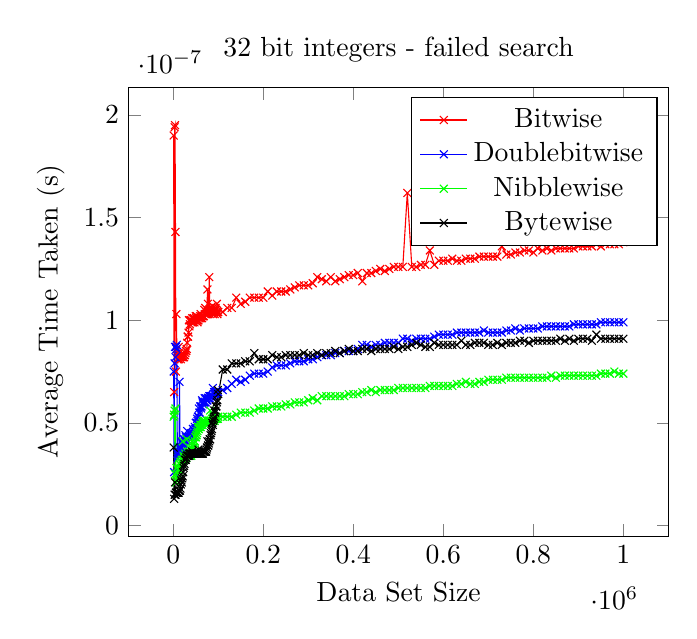
\begin{tikzpicture}
\begin{axis}[
xlabel=Data Set Size,
ylabel=Average Time Taken (s),
title=32 bit integers - failed search]
\addplot[color=red,mark=x] coordinates {
(1000,0.00000019
)
(2000,0.000000065
)
(3000,0.000000194
)
(4000,0.000000195
)
(5000,0.000000143
)
(6000,0.000000075
)
(7000,0.000000103
)
(8000,0.000000086
)
(9000,0.000000081
)
(10000,0.000000081
)
(11000,0.000000084
)
(12000,0.000000087
)
(13000,0.000000081
)
(14000,0.000000082
)
(15000,0.000000082
)
(16000,0.000000083
)
(17000,0.000000081
)
(18000,0.000000082
)
(19000,0.000000083
)
(20000,0.000000082
)
(21000,0.000000083
)
(22000,0.000000082
)
(23000,0.000000082
)
(24000,0.000000082
)
(25000,0.000000083
)
(26000,0.000000083
)
(27000,0.000000084
)
(28000,0.000000085
)
(29000,0.000000085
)
(30000,0.000000086
)
(31000,0.000000089
)
(32000,0.000000092
)
(33000,0.000000092
)
(34000,0.000000094
)
(35000,0.0000001
)
(36000,0.000000097
)
(37000,0.000000098
)
(38000,0.0000001
)
(39000,0.0000001
)
(40000,0.0000001
)
(41000,0.000000099
)
(42000,0.000000101
)
(43000,0.000000099
)
(44000,0.000000099
)
(45000,0.000000101
)
(46000,0.000000101
)
(47000,0.000000099
)
(48000,0.0000001
)
(49000,0.0000001
)
(50000,0.000000102
)
(51000,0.000000101
)
(52000,0.000000102
)
(53000,0.0000001
)
(54000,0.000000099
)
(55000,0.0000001
)
(56000,0.0000001
)
(57000,0.000000101
)
(58000,0.000000101
)
(59000,0.000000101
)
(60000,0.000000102
)
(61000,0.000000103
)
(62000,0.000000101
)
(63000,0.000000102
)
(64000,0.000000101
)
(65000,0.000000102
)
(66000,0.000000102
)
(67000,0.000000102
)
(68000,0.000000102
)
(69000,0.000000105
)
(70000,0.000000103
)
(71000,0.000000106
)
(72000,0.000000103
)
(73000,0.000000104
)
(74000,0.000000103
)
(75000,0.000000103
)
(76000,0.000000115
)
(77000,0.000000108
)
(78000,0.000000103
)
(79000,0.000000104
)
(80000,0.000000121
)
(81000,0.000000104
)
(82000,0.000000105
)
(83000,0.000000104
)
(84000,0.000000106
)
(85000,0.000000104
)
(86000,0.000000104
)
(87000,0.000000107
)
(88000,0.000000103
)
(89000,0.000000104
)
(90000,0.000000104
)
(91000,0.000000104
)
(92000,0.000000103
)
(93000,0.000000105
)
(94000,0.000000106
)
(95000,0.000000105
)
(96000,0.000000104
)
(97000,0.000000108
)
(98000,0.000000103
)
(99000,0.000000104
)
(100000,0.000000104
)
(110000,0.000000104
)
(120000,0.000000106
)
(130000,0.000000106
)
(140000,0.000000111
)
(150000,0.000000108
)
(160000,0.000000109
)
(170000,0.000000111
)
(180000,0.000000111
)
(190000,0.000000111
)
(200000,0.000000111
)
(210000,0.000000114
)
(220000,0.000000112
)
(230000,0.000000114
)
(240000,0.000000114
)
(250000,0.000000114
)
(260000,0.000000115
)
(270000,0.000000116
)
(280000,0.000000117
)
(290000,0.000000117
)
(300000,0.000000117
)
(310000,0.000000118
)
(320000,0.000000121
)
(330000,0.00000012
)
(340000,0.000000119
)
(350000,0.000000121
)
(360000,0.000000119
)
(370000,0.00000012
)
(380000,0.000000121
)
(390000,0.000000122
)
(400000,0.000000122
)
(410000,0.000000123
)
(420000,0.000000119
)
(430000,0.000000123
)
(440000,0.000000123
)
(450000,0.000000124
)
(460000,0.000000125
)
(470000,0.000000124
)
(480000,0.000000125
)
(490000,0.000000126
)
(500000,0.000000126
)
(510000,0.000000126
)
(520000,0.000000162
)
(530000,0.000000126
)
(540000,0.000000126
)
(550000,0.000000127
)
(560000,0.000000127
)
(570000,0.000000134
)
(580000,0.000000127
)
(590000,0.000000129
)
(600000,0.000000129
)
(610000,0.000000129
)
(620000,0.00000013
)
(630000,0.000000129
)
(640000,0.000000129
)
(650000,0.00000013
)
(660000,0.00000013
)
(670000,0.00000013
)
(680000,0.000000131
)
(690000,0.000000131
)
(700000,0.000000131
)
(710000,0.000000131
)
(720000,0.000000131
)
(730000,0.000000136
)
(740000,0.000000132
)
(750000,0.000000132
)
(760000,0.000000133
)
(770000,0.000000133
)
(780000,0.000000134
)
(790000,0.000000134
)
(800000,0.000000133
)
(810000,0.000000135
)
(820000,0.000000134
)
(830000,0.000000135
)
(840000,0.000000134
)
(850000,0.000000135
)
(860000,0.000000135
)
(870000,0.000000135
)
(880000,0.000000135
)
(890000,0.000000135
)
(900000,0.000000136
)
(910000,0.000000136
)
(920000,0.000000136
)
(930000,0.000000136
)
(940000,0.000000137
)
(950000,0.000000136
)
(960000,0.000000137
)
(970000,0.000000137
)
(980000,0.000000137
)
(990000,0.000000137
)
(1000000,0.000000138
)
};
\addlegendentry{Bitwise}
\addplot[color=blue,mark=x] coordinates {
(1000,0.000000075
)
(2000,0.000000026
)
(3000,0.000000079
)
(4000,0.000000087
)
(5000,0.000000082
)
(6000,0.000000087
)
(7000,0.000000086
)
(8000,0.000000088
)
(9000,0.000000035
)
(10000,0.000000033
)
(11000,0.000000034
)
(12000,0.000000035
)
(13000,0.000000036
)
(14000,0.00000007
)
(15000,0.000000038
)
(16000,0.000000037
)
(17000,0.000000038
)
(18000,0.000000041
)
(19000,0.000000038
)
(20000,0.00000004
)
(21000,0.000000039
)
(22000,0.00000004
)
(23000,0.00000004
)
(24000,0.000000042
)
(25000,0.000000042
)
(26000,0.000000041
)
(27000,0.000000044
)
(28000,0.000000043
)
(29000,0.000000041
)
(30000,0.000000042
)
(31000,0.000000046
)
(32000,0.000000043
)
(33000,0.000000043
)
(34000,0.000000043
)
(35000,0.000000043
)
(36000,0.000000043
)
(37000,0.000000043
)
(38000,0.000000044
)
(39000,0.000000045
)
(40000,0.000000044
)
(41000,0.000000044
)
(42000,0.000000044
)
(43000,0.000000045
)
(44000,0.000000047
)
(45000,0.000000045
)
(46000,0.000000046
)
(47000,0.000000046
)
(48000,0.000000048
)
(49000,0.000000047
)
(50000,0.00000005
)
(51000,0.00000005
)
(52000,0.00000005
)
(53000,0.000000052
)
(54000,0.000000051
)
(55000,0.000000053
)
(56000,0.000000053
)
(57000,0.000000057
)
(58000,0.000000055
)
(59000,0.000000055
)
(60000,0.000000058
)
(61000,0.000000058
)
(62000,0.000000057
)
(63000,0.000000058
)
(64000,0.000000061
)
(65000,0.00000006
)
(66000,0.000000059
)
(67000,0.00000006
)
(68000,0.00000006
)
(69000,0.00000006
)
(70000,0.000000062
)
(71000,0.00000006
)
(72000,0.00000006
)
(73000,0.000000062
)
(74000,0.000000061
)
(75000,0.000000061
)
(76000,0.000000061
)
(77000,0.000000062
)
(78000,0.000000062
)
(79000,0.000000062
)
(80000,0.000000063
)
(81000,0.000000062
)
(82000,0.000000063
)
(83000,0.000000063
)
(84000,0.000000063
)
(85000,0.000000063
)
(86000,0.000000063
)
(87000,0.000000063
)
(88000,0.000000067
)
(89000,0.000000063
)
(90000,0.000000064
)
(91000,0.000000065
)
(92000,0.000000065
)
(93000,0.000000064
)
(94000,0.000000065
)
(95000,0.000000064
)
(96000,0.000000065
)
(97000,0.000000064
)
(98000,0.000000065
)
(99000,0.000000065
)
(100000,0.000000065
)
(110000,0.000000066
)
(120000,0.000000067
)
(130000,0.000000069
)
(140000,0.000000071
)
(150000,0.00000007
)
(160000,0.000000071
)
(170000,0.000000073
)
(180000,0.000000074
)
(190000,0.000000074
)
(200000,0.000000074
)
(210000,0.000000075
)
(220000,0.000000077
)
(230000,0.000000078
)
(240000,0.000000078
)
(250000,0.000000078
)
(260000,0.000000079
)
(270000,0.00000008
)
(280000,0.00000008
)
(290000,0.00000008
)
(300000,0.000000081
)
(310000,0.000000081
)
(320000,0.000000082
)
(330000,0.000000083
)
(340000,0.000000083
)
(350000,0.000000083
)
(360000,0.000000084
)
(370000,0.000000084
)
(380000,0.000000085
)
(390000,0.000000085
)
(400000,0.000000085
)
(410000,0.000000086
)
(420000,0.000000088
)
(430000,0.000000088
)
(440000,0.000000087
)
(450000,0.000000088
)
(460000,0.000000088
)
(470000,0.000000089
)
(480000,0.000000089
)
(490000,0.000000089
)
(500000,0.000000089
)
(510000,0.000000091
)
(520000,0.000000091
)
(530000,0.00000009
)
(540000,0.000000091
)
(550000,0.000000091
)
(560000,0.000000091
)
(570000,0.000000091
)
(580000,0.000000092
)
(590000,0.000000093
)
(600000,0.000000093
)
(610000,0.000000093
)
(620000,0.000000093
)
(630000,0.000000094
)
(640000,0.000000094
)
(650000,0.000000094
)
(660000,0.000000094
)
(670000,0.000000094
)
(680000,0.000000094
)
(690000,0.000000095
)
(700000,0.000000094
)
(710000,0.000000094
)
(720000,0.000000094
)
(730000,0.000000094
)
(740000,0.000000095
)
(750000,0.000000095
)
(760000,0.000000096
)
(770000,0.000000095
)
(780000,0.000000096
)
(790000,0.000000096
)
(800000,0.000000096
)
(810000,0.000000096
)
(820000,0.000000097
)
(830000,0.000000097
)
(840000,0.000000097
)
(850000,0.000000097
)
(860000,0.000000097
)
(870000,0.000000097
)
(880000,0.000000097
)
(890000,0.000000098
)
(900000,0.000000098
)
(910000,0.000000098
)
(920000,0.000000098
)
(930000,0.000000098
)
(940000,0.000000098
)
(950000,0.000000099
)
(960000,0.000000099
)
(970000,0.000000099
)
(980000,0.000000099
)
(990000,0.000000099
)
(1000000,0.000000099
)
};
\addlegendentry{Doublebitwise}
\addplot[color=green,mark=x] coordinates {
(1000,0.000000053
)
(2000,0.000000054
)
(3000,0.000000056
)
(4000,0.000000025
)
(5000,0.000000057
)
(6000,0.000000021
)
(7000,0.000000028
)
(8000,0.000000022
)
(9000,0.000000023
)
(10000,0.000000025
)
(11000,0.000000027
)
(12000,0.000000027
)
(13000,0.000000028
)
(14000,0.00000003
)
(15000,0.00000003
)
(16000,0.000000031
)
(17000,0.000000031
)
(18000,0.000000031
)
(19000,0.000000032
)
(20000,0.000000032
)
(21000,0.000000041
)
(22000,0.000000032
)
(23000,0.000000034
)
(24000,0.000000033
)
(25000,0.000000032
)
(26000,0.000000033
)
(27000,0.000000035
)
(28000,0.000000033
)
(29000,0.000000033
)
(30000,0.000000042
)
(31000,0.000000036
)
(32000,0.000000034
)
(33000,0.000000034
)
(34000,0.000000035
)
(35000,0.000000036
)
(36000,0.000000034
)
(37000,0.000000035
)
(38000,0.000000034
)
(39000,0.000000037
)
(40000,0.000000034
)
(41000,0.000000041
)
(42000,0.000000036
)
(43000,0.000000037
)
(44000,0.000000037
)
(45000,0.000000038
)
(46000,0.00000004
)
(47000,0.00000004
)
(48000,0.000000041
)
(49000,0.000000043
)
(50000,0.000000043
)
(51000,0.000000044
)
(52000,0.000000044
)
(53000,0.000000045
)
(54000,0.000000046
)
(55000,0.000000048
)
(56000,0.000000047
)
(57000,0.000000047
)
(58000,0.000000048
)
(59000,0.000000048
)
(60000,0.000000049
)
(61000,0.000000048
)
(62000,0.000000049
)
(63000,0.000000049
)
(64000,0.00000005
)
(65000,0.000000049
)
(66000,0.000000051
)
(67000,0.00000005
)
(68000,0.000000051
)
(69000,0.000000051
)
(70000,0.00000005
)
(71000,0.00000005
)
(72000,0.00000005
)
(73000,0.00000005
)
(74000,0.00000005
)
(75000,0.000000051
)
(76000,0.000000051
)
(77000,0.000000051
)
(78000,0.000000051
)
(79000,0.000000051
)
(80000,0.000000051
)
(81000,0.000000051
)
(82000,0.000000056
)
(83000,0.000000051
)
(84000,0.000000051
)
(85000,0.000000051
)
(86000,0.000000052
)
(87000,0.000000052
)
(88000,0.000000051
)
(89000,0.000000052
)
(90000,0.000000052
)
(91000,0.000000052
)
(92000,0.000000051
)
(93000,0.000000052
)
(94000,0.000000052
)
(95000,0.000000052
)
(96000,0.000000052
)
(97000,0.000000052
)
(98000,0.000000052
)
(99000,0.000000052
)
(100000,0.000000053
)
(110000,0.000000053
)
(120000,0.000000053
)
(130000,0.000000053
)
(140000,0.000000054
)
(150000,0.000000055
)
(160000,0.000000055
)
(170000,0.000000055
)
(180000,0.000000056
)
(190000,0.000000057
)
(200000,0.000000057
)
(210000,0.000000057
)
(220000,0.000000058
)
(230000,0.000000058
)
(240000,0.000000058
)
(250000,0.000000059
)
(260000,0.000000059
)
(270000,0.00000006
)
(280000,0.00000006
)
(290000,0.00000006
)
(300000,0.000000061
)
(310000,0.000000062
)
(320000,0.000000061
)
(330000,0.000000063
)
(340000,0.000000063
)
(350000,0.000000063
)
(360000,0.000000063
)
(370000,0.000000063
)
(380000,0.000000063
)
(390000,0.000000064
)
(400000,0.000000064
)
(410000,0.000000064
)
(420000,0.000000065
)
(430000,0.000000065
)
(440000,0.000000066
)
(450000,0.000000065
)
(460000,0.000000066
)
(470000,0.000000066
)
(480000,0.000000066
)
(490000,0.000000066
)
(500000,0.000000067
)
(510000,0.000000067
)
(520000,0.000000067
)
(530000,0.000000067
)
(540000,0.000000067
)
(550000,0.000000067
)
(560000,0.000000067
)
(570000,0.000000068
)
(580000,0.000000068
)
(590000,0.000000068
)
(600000,0.000000068
)
(610000,0.000000068
)
(620000,0.000000068
)
(630000,0.000000069
)
(640000,0.000000069
)
(650000,0.00000007
)
(660000,0.000000069
)
(670000,0.000000069
)
(680000,0.00000007
)
(690000,0.00000007
)
(700000,0.000000071
)
(710000,0.000000071
)
(720000,0.000000071
)
(730000,0.000000071
)
(740000,0.000000072
)
(750000,0.000000072
)
(760000,0.000000072
)
(770000,0.000000072
)
(780000,0.000000072
)
(790000,0.000000072
)
(800000,0.000000072
)
(810000,0.000000072
)
(820000,0.000000072
)
(830000,0.000000072
)
(840000,0.000000073
)
(850000,0.000000072
)
(860000,0.000000073
)
(870000,0.000000073
)
(880000,0.000000073
)
(890000,0.000000073
)
(900000,0.000000073
)
(910000,0.000000073
)
(920000,0.000000073
)
(930000,0.000000073
)
(940000,0.000000073
)
(950000,0.000000074
)
(960000,0.000000074
)
(970000,0.000000074
)
(980000,0.000000075
)
(990000,0.000000074
)
(1000000,0.000000074
)
};
\addlegendentry{Nibblewise}
\addplot[color=black,mark=x] coordinates {
(1000,0.000000038
)
(2000,0.000000013
)
(3000,0.000000015
)
(4000,0.000000021
)
(5000,0.000000015
)
(6000,0.000000016
)
(7000,0.000000016
)
(8000,0.000000016
)
(9000,0.000000016
)
(10000,0.000000016
)
(11000,0.000000016
)
(12000,0.000000016
)
(13000,0.000000017
)
(14000,0.000000017
)
(15000,0.000000017
)
(16000,0.000000018
)
(17000,0.00000002
)
(18000,0.000000022
)
(19000,0.000000021
)
(20000,0.000000023
)
(21000,0.000000024
)
(22000,0.000000026
)
(23000,0.000000028
)
(24000,0.000000029
)
(25000,0.00000003
)
(26000,0.000000032
)
(27000,0.000000032
)
(28000,0.000000032
)
(29000,0.000000033
)
(30000,0.000000034
)
(31000,0.000000034
)
(32000,0.000000034
)
(33000,0.000000034
)
(34000,0.000000034
)
(35000,0.000000035
)
(36000,0.000000034
)
(37000,0.000000035
)
(38000,0.000000035
)
(39000,0.000000035
)
(40000,0.000000035
)
(41000,0.000000035
)
(42000,0.000000036
)
(43000,0.000000035
)
(44000,0.000000035
)
(45000,0.000000035
)
(46000,0.000000035
)
(47000,0.000000035
)
(48000,0.000000035
)
(49000,0.000000035
)
(50000,0.000000035
)
(51000,0.000000035
)
(52000,0.000000035
)
(53000,0.000000035
)
(54000,0.000000035
)
(55000,0.000000035
)
(56000,0.000000037
)
(57000,0.000000035
)
(58000,0.000000035
)
(59000,0.000000035
)
(60000,0.000000035
)
(61000,0.000000035
)
(62000,0.000000035
)
(63000,0.000000035
)
(64000,0.000000035
)
(65000,0.000000035
)
(66000,0.000000035
)
(67000,0.000000036
)
(68000,0.000000036
)
(69000,0.000000036
)
(70000,0.000000036
)
(71000,0.000000036
)
(72000,0.000000036
)
(73000,0.000000036
)
(74000,0.000000037
)
(75000,0.000000038
)
(76000,0.000000041
)
(77000,0.000000039
)
(78000,0.000000039
)
(79000,0.00000004
)
(80000,0.000000041
)
(81000,0.000000042
)
(82000,0.000000042
)
(83000,0.000000044
)
(84000,0.000000045
)
(85000,0.000000046
)
(86000,0.000000047
)
(87000,0.00000005
)
(88000,0.000000049
)
(89000,0.000000051
)
(90000,0.000000052
)
(91000,0.000000056
)
(92000,0.000000053
)
(93000,0.000000055
)
(94000,0.000000056
)
(95000,0.000000058
)
(96000,0.000000058
)
(97000,0.00000006
)
(98000,0.000000061
)
(99000,0.000000066
)
(100000,0.000000064
)
(110000,0.000000076
)
(120000,0.000000076
)
(130000,0.000000079
)
(140000,0.000000079
)
(150000,0.000000079
)
(160000,0.00000008
)
(170000,0.00000008
)
(180000,0.000000084
)
(190000,0.000000081
)
(200000,0.000000081
)
(210000,0.000000081
)
(220000,0.000000083
)
(230000,0.000000082
)
(240000,0.000000082
)
(250000,0.000000083
)
(260000,0.000000083
)
(270000,0.000000083
)
(280000,0.000000083
)
(290000,0.000000084
)
(300000,0.000000083
)
(310000,0.000000083
)
(320000,0.000000084
)
(330000,0.000000083
)
(340000,0.000000084
)
(350000,0.000000084
)
(360000,0.000000085
)
(370000,0.000000084
)
(380000,0.000000085
)
(390000,0.000000086
)
(400000,0.000000085
)
(410000,0.000000085
)
(420000,0.000000086
)
(430000,0.000000086
)
(440000,0.000000085
)
(450000,0.000000086
)
(460000,0.000000086
)
(470000,0.000000086
)
(480000,0.000000086
)
(490000,0.000000087
)
(500000,0.000000086
)
(510000,0.000000087
)
(520000,0.000000087
)
(530000,0.000000088
)
(540000,0.000000089
)
(550000,0.000000088
)
(560000,0.000000087
)
(570000,0.000000087
)
(580000,0.000000089
)
(590000,0.000000088
)
(600000,0.000000088
)
(610000,0.000000088
)
(620000,0.000000088
)
(630000,0.000000088
)
(640000,0.00000009
)
(650000,0.000000088
)
(660000,0.000000088
)
(670000,0.000000089
)
(680000,0.000000089
)
(690000,0.000000089
)
(700000,0.000000088
)
(710000,0.000000088
)
(720000,0.000000089
)
(730000,0.000000088
)
(740000,0.000000089
)
(750000,0.000000089
)
(760000,0.000000089
)
(770000,0.00000009
)
(780000,0.00000009
)
(790000,0.000000089
)
(800000,0.00000009
)
(810000,0.00000009
)
(820000,0.00000009
)
(830000,0.00000009
)
(840000,0.00000009
)
(850000,0.00000009
)
(860000,0.000000091
)
(870000,0.00000009
)
(880000,0.000000091
)
(890000,0.00000009
)
(900000,0.000000091
)
(910000,0.000000091
)
(920000,0.000000091
)
(930000,0.00000009
)
(940000,0.000000093
)
(950000,0.000000091
)
(960000,0.000000091
)
(970000,0.000000091
)
(980000,0.000000091
)
(990000,0.000000091
)
(1000000,0.000000091
)
};
\addlegendentry{Bytewise}
\end{axis}
\end{tikzpicture}

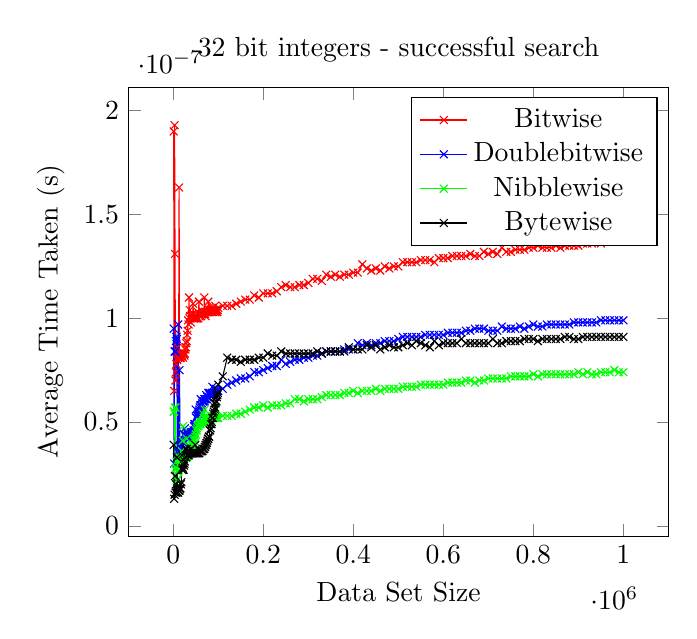
\begin{tikzpicture}
\begin{axis}[
xlabel=Data Set Size,
ylabel=Average Time Taken (s),
title=32 bit integers - successful search]
\addplot[color=red,mark=x] coordinates {
(1000,0.00000019)
(2000,0.000000065)
(3000,0.000000193)
(4000,0.000000131)
(5000,0.00000007)
(6000,0.000000074)
(7000,0.000000078)
(8000,0.00000008)
(9000,0.00000008)
(10000,0.000000086)
(11000,0.000000081)
(12000,0.000000081)
(13000,0.000000163)
(14000,0.000000083)
(15000,0.000000081)
(16000,0.000000082)
(17000,0.000000081)
(18000,0.000000082)
(19000,0.000000082)
(20000,0.000000082)
(21000,0.000000083)
(22000,0.000000081)
(23000,0.000000083)
(24000,0.000000083)
(25000,0.000000082)
(26000,0.000000083)
(27000,0.000000085)
(28000,0.000000086)
(29000,0.000000088)
(30000,0.000000089)
(31000,0.000000092)
(32000,0.000000094)
(33000,0.000000099)
(34000,0.000000097)
(35000,0.00000011)
(36000,0.0000001)
(37000,0.000000104)
(38000,0.000000101)
(39000,0.000000098)
(40000,0.000000101)
(41000,0.000000101)
(42000,0.000000102)
(43000,0.0000001)
(44000,0.000000107)
(45000,0.0000001)
(46000,0.0000001)
(47000,0.0000001)
(48000,0.0000001)
(49000,0.000000101)
(50000,0.0000001)
(51000,0.000000101)
(52000,0.0000001)
(53000,0.0000001)
(54000,0.0000001)
(55000,0.000000103)
(56000,0.0000001)
(57000,0.000000108)
(58000,0.000000102)
(59000,0.000000101)
(60000,0.000000101)
(61000,0.000000102)
(62000,0.000000101)
(63000,0.000000102)
(64000,0.000000102)
(65000,0.000000103)
(66000,0.000000103)
(67000,0.000000102)
(68000,0.000000102)
(69000,0.00000011)
(70000,0.000000103)
(71000,0.000000102)
(72000,0.000000101)
(73000,0.000000103)
(74000,0.000000103)
(75000,0.000000103)
(76000,0.000000103)
(77000,0.000000103)
(78000,0.000000108)
(79000,0.000000104)
(80000,0.000000103)
(81000,0.000000104)
(82000,0.000000104)
(83000,0.000000104)
(84000,0.000000104)
(85000,0.000000104)
(86000,0.000000103)
(87000,0.000000105)
(88000,0.000000103)
(89000,0.000000104)
(90000,0.000000104)
(91000,0.000000104)
(92000,0.000000103)
(93000,0.000000106)
(94000,0.000000103)
(95000,0.000000104)
(96000,0.000000104)
(97000,0.000000103)
(98000,0.000000103)
(99000,0.000000104)
(100000,0.000000105)
(110000,0.000000106)
(120000,0.000000106)
(130000,0.000000106)
(140000,0.000000107)
(150000,0.000000108)
(160000,0.000000109)
(170000,0.000000109)
(180000,0.000000111)
(190000,0.00000011)
(200000,0.000000112)
(210000,0.000000112)
(220000,0.000000112)
(230000,0.000000113)
(240000,0.000000115)
(250000,0.000000116)
(260000,0.000000115)
(270000,0.000000115)
(280000,0.000000116)
(290000,0.000000116)
(300000,0.000000117)
(310000,0.000000119)
(320000,0.000000119)
(330000,0.000000118)
(340000,0.000000121)
(350000,0.00000012)
(360000,0.000000121)
(370000,0.00000012)
(380000,0.000000121)
(390000,0.000000121)
(400000,0.000000122)
(410000,0.000000122)
(420000,0.000000126)
(430000,0.000000124)
(440000,0.000000123)
(450000,0.000000124)
(460000,0.000000123)
(470000,0.000000125)
(480000,0.000000124)
(490000,0.000000125)
(500000,0.000000125)
(510000,0.000000127)
(520000,0.000000127)
(530000,0.000000127)
(540000,0.000000127)
(550000,0.000000128)
(560000,0.000000128)
(570000,0.000000128)
(580000,0.000000127)
(590000,0.000000129)
(600000,0.000000129)
(610000,0.000000129)
(620000,0.00000013)
(630000,0.00000013)
(640000,0.00000013)
(650000,0.00000013)
(660000,0.000000131)
(670000,0.00000013)
(680000,0.00000013)
(690000,0.000000132)
(700000,0.000000131)
(710000,0.000000132)
(720000,0.000000131)
(730000,0.000000134)
(740000,0.000000132)
(750000,0.000000132)
(760000,0.000000133)
(770000,0.000000133)
(780000,0.000000133)
(790000,0.000000134)
(800000,0.000000134)
(810000,0.000000135)
(820000,0.000000134)
(830000,0.000000134)
(840000,0.000000134)
(850000,0.000000135)
(860000,0.000000134)
(870000,0.000000135)
(880000,0.000000135)
(890000,0.000000135)
(900000,0.000000135)
(910000,0.000000136)
(920000,0.000000136)
(930000,0.000000136)
(940000,0.000000137)
(950000,0.000000136)
(960000,0.000000137)
(970000,0.000000137)
(980000,0.000000137)
(990000,0.000000137)
(1000000,0.000000137)
};
\addlegendentry{Bitwise}
\addplot[color=blue,mark=x] coordinates {
(1000,0.000000095)
(2000,0.00000003)
(3000,0.000000084)
(4000,0.000000084)
(5000,0.000000084)
(6000,0.000000089)
(7000,0.000000091)
(8000,0.00000009)
(9000,0.000000033)
(10000,0.000000036)
(11000,0.000000097)
(12000,0.000000035)
(13000,0.000000036)
(14000,0.000000075)
(15000,0.000000038)
(16000,0.000000038)
(17000,0.000000038)
(18000,0.000000038)
(19000,0.000000041)
(20000,0.000000039)
(21000,0.000000039)
(22000,0.00000004)
(23000,0.000000041)
(24000,0.000000044)
(25000,0.000000044)
(26000,0.000000047)
(27000,0.000000043)
(28000,0.000000042)
(29000,0.000000042)
(30000,0.000000045)
(31000,0.000000043)
(32000,0.000000042)
(33000,0.000000043)
(34000,0.000000044)
(35000,0.000000043)
(36000,0.000000043)
(37000,0.000000043)
(38000,0.000000044)
(39000,0.000000045)
(40000,0.000000045)
(41000,0.000000044)
(42000,0.000000045)
(43000,0.000000045)
(44000,0.000000045)
(45000,0.000000046)
(46000,0.000000048)
(47000,0.000000049)
(48000,0.000000048)
(49000,0.000000049)
(50000,0.000000056)
(51000,0.000000052)
(52000,0.000000052)
(53000,0.000000053)
(54000,0.000000053)
(55000,0.000000054)
(56000,0.000000055)
(57000,0.000000055)
(58000,0.000000056)
(59000,0.000000057)
(60000,0.000000058)
(61000,0.000000061)
(62000,0.000000058)
(63000,0.000000058)
(64000,0.000000059)
(65000,0.00000006)
(66000,0.00000006)
(67000,0.00000006)
(68000,0.00000006)
(69000,0.000000061)
(70000,0.00000006)
(71000,0.000000061)
(72000,0.000000061)
(73000,0.000000063)
(74000,0.000000061)
(75000,0.000000061)
(76000,0.000000062)
(77000,0.000000062)
(78000,0.000000064)
(79000,0.000000062)
(80000,0.000000064)
(81000,0.000000063)
(82000,0.000000064)
(83000,0.000000063)
(84000,0.000000063)
(85000,0.000000063)
(86000,0.000000064)
(87000,0.000000067)
(88000,0.000000063)
(89000,0.000000063)
(90000,0.000000064)
(91000,0.000000066)
(92000,0.000000064)
(93000,0.000000064)
(94000,0.000000064)
(95000,0.000000066)
(96000,0.000000065)
(97000,0.000000065)
(98000,0.000000065)
(99000,0.000000065)
(100000,0.000000065)
(110000,0.000000066)
(120000,0.000000068)
(130000,0.000000069)
(140000,0.00000007)
(150000,0.000000071)
(160000,0.000000071)
(170000,0.000000072)
(180000,0.000000074)
(190000,0.000000074)
(200000,0.000000075)
(210000,0.000000076)
(220000,0.000000077)
(230000,0.000000077)
(240000,0.00000008)
(250000,0.000000078)
(260000,0.000000079)
(270000,0.00000008)
(280000,0.00000008)
(290000,0.000000081)
(300000,0.000000081)
(310000,0.000000082)
(320000,0.000000082)
(330000,0.000000083)
(340000,0.000000084)
(350000,0.000000084)
(360000,0.000000084)
(370000,0.000000084)
(380000,0.000000085)
(390000,0.000000085)
(400000,0.000000085)
(410000,0.000000088)
(420000,0.000000087)
(430000,0.000000088)
(440000,0.000000087)
(450000,0.000000088)
(460000,0.000000088)
(470000,0.000000089)
(480000,0.000000089)
(490000,0.000000089)
(500000,0.00000009)
(510000,0.000000091)
(520000,0.000000091)
(530000,0.000000091)
(540000,0.000000091)
(550000,0.000000091)
(560000,0.000000092)
(570000,0.000000092)
(580000,0.000000092)
(590000,0.000000092)
(600000,0.000000092)
(610000,0.000000093)
(620000,0.000000093)
(630000,0.000000093)
(640000,0.000000093)
(650000,0.000000094)
(660000,0.000000094)
(670000,0.000000095)
(680000,0.000000095)
(690000,0.000000095)
(700000,0.000000094)
(710000,0.000000094)
(720000,0.000000094)
(730000,0.000000096)
(740000,0.000000095)
(750000,0.000000095)
(760000,0.000000095)
(770000,0.000000096)
(780000,0.000000095)
(790000,0.000000096)
(800000,0.000000097)
(810000,0.000000096)
(820000,0.000000096)
(830000,0.000000097)
(840000,0.000000097)
(850000,0.000000097)
(860000,0.000000097)
(870000,0.000000097)
(880000,0.000000097)
(890000,0.000000098)
(900000,0.000000098)
(910000,0.000000098)
(920000,0.000000098)
(930000,0.000000098)
(940000,0.000000098)
(950000,0.000000099)
(960000,0.000000099)
(970000,0.000000099)
(980000,0.000000099)
(990000,0.000000099)
(1000000,0.000000099)
};
\addlegendentry{Doublebitwise}
\addplot[color=green,mark=x] coordinates {
(1000,0.000000055)
(2000,0.000000055)
(3000,0.000000057)
(4000,0.000000027)
(5000,0.000000057)
(6000,0.000000028)
(7000,0.000000031)
(8000,0.000000022)
(9000,0.000000022)
(10000,0.000000026)
(11000,0.000000026)
(12000,0.000000027)
(13000,0.000000029)
(14000,0.000000033)
(15000,0.000000032)
(16000,0.000000031)
(17000,0.000000031)
(18000,0.000000034)
(19000,0.000000036)
(20000,0.000000032)
(21000,0.000000041)
(22000,0.000000048)
(23000,0.000000032)
(24000,0.000000032)
(25000,0.000000034)
(26000,0.000000034)
(27000,0.000000033)
(28000,0.000000033)
(29000,0.000000033)
(30000,0.000000042)
(31000,0.000000033)
(32000,0.000000034)
(33000,0.000000034)
(34000,0.000000035)
(35000,0.000000034)
(36000,0.000000035)
(37000,0.000000036)
(38000,0.000000035)
(39000,0.000000038)
(40000,0.000000037)
(41000,0.000000036)
(42000,0.000000039)
(43000,0.000000038)
(44000,0.000000039)
(45000,0.000000039)
(46000,0.000000041)
(47000,0.000000042)
(48000,0.000000042)
(49000,0.000000043)
(50000,0.000000044)
(51000,0.000000046)
(52000,0.000000046)
(53000,0.000000047)
(54000,0.000000048)
(55000,0.000000048)
(56000,0.000000048)
(57000,0.000000049)
(58000,0.000000049)
(59000,0.000000049)
(60000,0.00000005)
(61000,0.000000049)
(62000,0.00000005)
(63000,0.00000005)
(64000,0.00000005)
(65000,0.00000005)
(66000,0.000000054)
(67000,0.00000005)
(68000,0.000000052)
(69000,0.000000052)
(70000,0.000000056)
(71000,0.000000051)
(72000,0.000000051)
(73000,0.000000051)
(74000,0.000000051)
(75000,0.000000052)
(76000,0.000000052)
(77000,0.000000052)
(78000,0.000000051)
(79000,0.000000051)
(80000,0.000000051)
(81000,0.000000051)
(82000,0.000000052)
(83000,0.000000051)
(84000,0.000000051)
(85000,0.000000052)
(86000,0.000000052)
(87000,0.000000053)
(88000,0.000000052)
(89000,0.000000053)
(90000,0.000000052)
(91000,0.000000052)
(92000,0.000000052)
(93000,0.000000052)
(94000,0.000000052)
(95000,0.000000056)
(96000,0.000000052)
(97000,0.000000052)
(98000,0.000000052)
(99000,0.000000052)
(100000,0.000000052)
(110000,0.000000053)
(120000,0.000000053)
(130000,0.000000053)
(140000,0.000000054)
(150000,0.000000054)
(160000,0.000000055)
(170000,0.000000056)
(180000,0.000000057)
(190000,0.000000057)
(200000,0.000000058)
(210000,0.000000057)
(220000,0.000000058)
(230000,0.000000058)
(240000,0.000000058)
(250000,0.000000059)
(260000,0.000000059)
(270000,0.000000061)
(280000,0.000000061)
(290000,0.00000006)
(300000,0.000000061)
(310000,0.000000061)
(320000,0.000000061)
(330000,0.000000062)
(340000,0.000000063)
(350000,0.000000063)
(360000,0.000000063)
(370000,0.000000063)
(380000,0.000000064)
(390000,0.000000064)
(400000,0.000000065)
(410000,0.000000064)
(420000,0.000000065)
(430000,0.000000065)
(440000,0.000000065)
(450000,0.000000066)
(460000,0.000000065)
(470000,0.000000066)
(480000,0.000000066)
(490000,0.000000066)
(500000,0.000000066)
(510000,0.000000067)
(520000,0.000000067)
(530000,0.000000067)
(540000,0.000000067)
(550000,0.000000068)
(560000,0.000000068)
(570000,0.000000068)
(580000,0.000000068)
(590000,0.000000068)
(600000,0.000000068)
(610000,0.000000069)
(620000,0.000000069)
(630000,0.000000069)
(640000,0.000000069)
(650000,0.00000007)
(660000,0.00000007)
(670000,0.000000069)
(680000,0.00000007)
(690000,0.00000007)
(700000,0.000000071)
(710000,0.000000071)
(720000,0.000000071)
(730000,0.000000071)
(740000,0.000000071)
(750000,0.000000072)
(760000,0.000000072)
(770000,0.000000072)
(780000,0.000000072)
(790000,0.000000072)
(800000,0.000000073)
(810000,0.000000072)
(820000,0.000000073)
(830000,0.000000073)
(840000,0.000000073)
(850000,0.000000073)
(860000,0.000000073)
(870000,0.000000073)
(880000,0.000000073)
(890000,0.000000073)
(900000,0.000000074)
(910000,0.000000073)
(920000,0.000000074)
(930000,0.000000073)
(940000,0.000000073)
(950000,0.000000074)
(960000,0.000000074)
(970000,0.000000074)
(980000,0.000000075)
(990000,0.000000074)
(1000000,0.000000074)
};
\addlegendentry{Nibblewise}
\addplot[color=black,mark=x] coordinates {
(1000,0.000000039)
(2000,0.000000013)
(3000,0.000000015)
(4000,0.000000024)
(5000,0.000000016)
(6000,0.00000002)
(7000,0.000000016)
(8000,0.000000033)
(9000,0.000000018)
(10000,0.000000016)
(11000,0.000000016)
(12000,0.000000017)
(13000,0.000000017)
(14000,0.000000017)
(15000,0.000000018)
(16000,0.000000018)
(17000,0.00000002)
(18000,0.000000021)
(19000,0.000000034)
(20000,0.000000027)
(21000,0.000000028)
(22000,0.000000027)
(23000,0.000000027)
(24000,0.000000029)
(25000,0.00000003)
(26000,0.000000031)
(27000,0.000000037)
(28000,0.000000037)
(29000,0.000000033)
(30000,0.000000037)
(31000,0.000000034)
(32000,0.000000036)
(33000,0.000000034)
(34000,0.000000034)
(35000,0.000000035)
(36000,0.000000035)
(37000,0.000000035)
(38000,0.000000035)
(39000,0.000000037)
(40000,0.000000035)
(41000,0.000000035)
(42000,0.000000035)
(43000,0.000000035)
(44000,0.000000035)
(45000,0.000000035)
(46000,0.000000035)
(47000,0.000000035)
(48000,0.000000035)
(49000,0.000000039)
(50000,0.000000035)
(51000,0.000000035)
(52000,0.000000035)
(53000,0.000000035)
(54000,0.000000035)
(55000,0.000000035)
(56000,0.000000037)
(57000,0.000000035)
(58000,0.000000035)
(59000,0.000000036)
(60000,0.000000036)
(61000,0.000000036)
(62000,0.000000036)
(63000,0.000000036)
(64000,0.000000036)
(65000,0.000000036)
(66000,0.000000037)
(67000,0.000000037)
(68000,0.000000037)
(69000,0.000000037)
(70000,0.000000038)
(71000,0.000000038)
(72000,0.000000039)
(73000,0.000000039)
(74000,0.00000004)
(75000,0.00000004)
(76000,0.000000041)
(77000,0.000000042)
(78000,0.000000042)
(79000,0.000000043)
(80000,0.000000043)
(81000,0.000000046)
(82000,0.000000046)
(83000,0.000000047)
(84000,0.000000049)
(85000,0.000000049)
(86000,0.00000005)
(87000,0.000000052)
(88000,0.000000052)
(89000,0.000000054)
(90000,0.000000055)
(91000,0.000000059)
(92000,0.000000056)
(93000,0.000000057)
(94000,0.000000059)
(95000,0.00000006)
(96000,0.00000006)
(97000,0.000000062)
(98000,0.000000063)
(99000,0.000000064)
(100000,0.000000068)
(110000,0.000000072)
(120000,0.000000081)
(130000,0.00000008)
(140000,0.00000008)
(150000,0.000000079)
(160000,0.00000008)
(170000,0.00000008)
(180000,0.00000008)
(190000,0.000000081)
(200000,0.000000081)
(210000,0.000000083)
(220000,0.000000082)
(230000,0.000000082)
(240000,0.000000084)
(250000,0.000000083)
(260000,0.000000083)
(270000,0.000000083)
(280000,0.000000083)
(290000,0.000000083)
(300000,0.000000083)
(310000,0.000000083)
(320000,0.000000084)
(330000,0.000000083)
(340000,0.000000084)
(350000,0.000000084)
(360000,0.000000084)
(370000,0.000000084)
(380000,0.000000084)
(390000,0.000000086)
(400000,0.000000085)
(410000,0.000000085)
(420000,0.000000085)
(430000,0.000000087)
(440000,0.000000086)
(450000,0.000000087)
(460000,0.000000085)
(470000,0.000000086)
(480000,0.000000087)
(490000,0.000000086)
(500000,0.000000086)
(510000,0.000000087)
(520000,0.000000088)
(530000,0.000000087)
(540000,0.000000089)
(550000,0.000000088)
(560000,0.000000087)
(570000,0.000000086)
(580000,0.000000089)
(590000,0.000000087)
(600000,0.000000088)
(610000,0.000000088)
(620000,0.000000088)
(630000,0.000000088)
(640000,0.00000009)
(650000,0.000000088)
(660000,0.000000088)
(670000,0.000000088)
(680000,0.000000088)
(690000,0.000000088)
(700000,0.000000088)
(710000,0.00000009)
(720000,0.000000088)
(730000,0.000000088)
(740000,0.000000089)
(750000,0.000000089)
(760000,0.000000089)
(770000,0.000000089)
(780000,0.00000009)
(790000,0.00000009)
(800000,0.00000009)
(810000,0.000000089)
(820000,0.00000009)
(830000,0.00000009)
(840000,0.00000009)
(850000,0.00000009)
(860000,0.00000009)
(870000,0.000000091)
(880000,0.000000091)
(890000,0.00000009)
(900000,0.00000009)
(910000,0.000000091)
(920000,0.000000091)
(930000,0.000000091)
(940000,0.000000091)
(950000,0.000000091)
(960000,0.000000091)
(970000,0.000000091)
(980000,0.000000091)
(990000,0.000000091)
(1000000,0.000000091)
};
\addlegendentry{Bytewise}
\end{axis}
\end{tikzpicture}

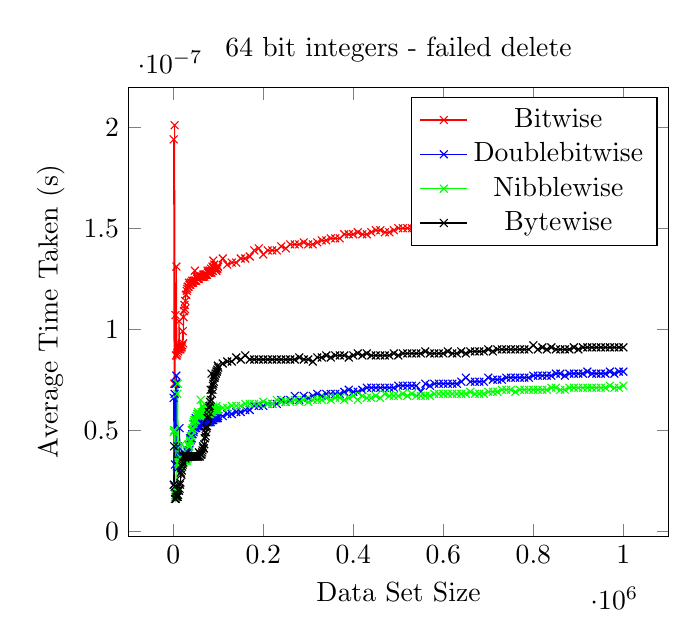
\begin{tikzpicture}
\begin{axis}[
xlabel=Data Set Size,
ylabel=Average Time Taken (s),
title=64 bit integers - failed delete]
\addplot[color=red,mark=x] coordinates {
(1000,0.000000194)
(2000,0.000000073)
(3000,0.000000201)
(4000,0.000000073)
(5000,0.000000107)
(6000,0.000000087)
(7000,0.000000131)
(8000,0.000000087)
(9000,0.000000088)
(10000,0.000000092)
(11000,0.000000089)
(12000,0.00000009)
(13000,0.000000104)
(14000,0.000000091)
(15000,0.00000009)
(16000,0.00000009)
(17000,0.000000091)
(18000,0.000000092)
(19000,0.000000091)
(20000,0.000000092)
(21000,0.000000099)
(22000,0.000000093)
(23000,0.000000106)
(24000,0.000000109)
(25000,0.000000112)
(26000,0.00000011)
(27000,0.000000114)
(28000,0.000000117)
(29000,0.000000117)
(30000,0.000000119)
(31000,0.00000012)
(32000,0.000000121)
(33000,0.000000121)
(34000,0.000000121)
(35000,0.000000123)
(36000,0.000000122)
(37000,0.000000122)
(38000,0.000000122)
(39000,0.000000123)
(40000,0.000000123)
(41000,0.000000123)
(42000,0.000000124)
(43000,0.000000123)
(44000,0.000000123)
(45000,0.000000124)
(46000,0.000000124)
(47000,0.000000124)
(48000,0.000000129)
(49000,0.000000124)
(50000,0.000000124)
(51000,0.000000124)
(52000,0.000000126)
(53000,0.000000125)
(54000,0.000000125)
(55000,0.000000125)
(56000,0.000000125)
(57000,0.000000125)
(58000,0.000000126)
(59000,0.000000126)
(60000,0.000000126)
(61000,0.000000126)
(62000,0.000000126)
(63000,0.000000126)
(64000,0.000000126)
(65000,0.000000126)
(66000,0.000000126)
(67000,0.000000127)
(68000,0.000000127)
(69000,0.000000126)
(70000,0.000000127)
(71000,0.000000127)
(72000,0.000000127)
(73000,0.000000127)
(74000,0.000000127)
(75000,0.000000127)
(76000,0.000000129)
(77000,0.000000128)
(78000,0.000000128)
(79000,0.000000128)
(80000,0.000000129)
(81000,0.000000128)
(82000,0.000000129)
(83000,0.000000128)
(84000,0.00000013)
(85000,0.000000128)
(86000,0.000000129)
(87000,0.000000131)
(88000,0.000000129)
(89000,0.000000134)
(90000,0.00000013)
(91000,0.000000132)
(92000,0.00000013)
(93000,0.00000013)
(94000,0.00000013)
(95000,0.000000129)
(96000,0.000000129)
(97000,0.00000013)
(98000,0.00000013)
(99000,0.000000131)
(100000,0.000000131)
(110000,0.000000135)
(120000,0.000000132)
(130000,0.000000133)
(140000,0.000000133)
(150000,0.000000135)
(160000,0.000000135)
(170000,0.000000136)
(180000,0.000000139)
(190000,0.00000014)
(200000,0.000000137)
(210000,0.000000139)
(220000,0.000000139)
(230000,0.000000139)
(240000,0.000000141)
(250000,0.00000014)
(260000,0.000000142)
(270000,0.000000142)
(280000,0.000000142)
(290000,0.000000143)
(300000,0.000000142)
(310000,0.000000142)
(320000,0.000000143)
(330000,0.000000144)
(340000,0.000000144)
(350000,0.000000145)
(360000,0.000000145)
(370000,0.000000145)
(380000,0.000000147)
(390000,0.000000147)
(400000,0.000000147)
(410000,0.000000148)
(420000,0.000000147)
(430000,0.000000147)
(440000,0.000000148)
(450000,0.000000149)
(460000,0.000000149)
(470000,0.000000148)
(480000,0.000000148)
(490000,0.000000149)
(500000,0.00000015)
(510000,0.00000015)
(520000,0.00000015)
(530000,0.00000015)
(540000,0.00000015)
(550000,0.00000015)
(560000,0.000000151)
(570000,0.000000151)
(580000,0.000000151)
(590000,0.000000151)
(600000,0.000000152)
(610000,0.000000152)
(620000,0.000000152)
(630000,0.000000152)
(640000,0.000000153)
(650000,0.000000153)
(660000,0.000000153)
(670000,0.000000153)
(680000,0.000000154)
(690000,0.000000153)
(700000,0.000000154)
(710000,0.000000155)
(720000,0.000000154)
(730000,0.000000154)
(740000,0.000000154)
(750000,0.000000155)
(760000,0.000000155)
(770000,0.000000155)
(780000,0.000000155)
(790000,0.000000156)
(800000,0.000000156)
(810000,0.000000156)
(820000,0.000000156)
(830000,0.000000156)
(840000,0.000000156)
(850000,0.000000156)
(860000,0.000000156)
(870000,0.000000157)
(880000,0.000000157)
(890000,0.000000157)
(900000,0.000000157)
(910000,0.000000158)
(920000,0.000000157)
(930000,0.000000157)
(940000,0.000000157)
(950000,0.000000158)
(960000,0.000000158)
(970000,0.000000158)
(980000,0.000000158)
(990000,0.000000158)
(1000000,0.000000158)
};
\addlegendentry{Bitwise}
\addplot[color=blue,mark=x] coordinates {
(1000,0.000000066)
(2000,0.000000023)
(3000,0.000000068)
(4000,0.000000033)
(5000,0.000000073)
(6000,0.000000073)
(7000,0.000000077)
(8000,0.000000032)
(9000,0.000000031)
(10000,0.000000042)
(11000,0.000000033)
(12000,0.000000035)
(13000,0.000000034)
(14000,0.000000051)
(15000,0.000000036)
(16000,0.000000034)
(17000,0.000000035)
(18000,0.000000037)
(19000,0.000000035)
(20000,0.000000035)
(21000,0.000000035)
(22000,0.000000036)
(23000,0.000000036)
(24000,0.000000036)
(25000,0.000000036)
(26000,0.000000038)
(27000,0.000000036)
(28000,0.000000037)
(29000,0.000000038)
(30000,0.000000037)
(31000,0.00000004)
(32000,0.000000039)
(33000,0.000000039)
(34000,0.000000038)
(35000,0.00000004)
(36000,0.00000004)
(37000,0.000000046)
(38000,0.000000045)
(39000,0.000000045)
(40000,0.000000046)
(41000,0.000000046)
(42000,0.000000048)
(43000,0.000000048)
(44000,0.00000005)
(45000,0.000000049)
(46000,0.00000005)
(47000,0.000000053)
(48000,0.000000051)
(49000,0.000000052)
(50000,0.000000056)
(51000,0.000000051)
(52000,0.000000054)
(53000,0.000000052)
(54000,0.000000052)
(55000,0.000000052)
(56000,0.000000052)
(57000,0.000000052)
(58000,0.000000052)
(59000,0.000000054)
(60000,0.000000052)
(61000,0.000000053)
(62000,0.000000053)
(63000,0.000000057)
(64000,0.000000053)
(65000,0.000000053)
(66000,0.000000053)
(67000,0.000000053)
(68000,0.000000053)
(69000,0.000000054)
(70000,0.000000054)
(71000,0.000000054)
(72000,0.000000054)
(73000,0.000000054)
(74000,0.000000054)
(75000,0.000000054)
(76000,0.000000054)
(77000,0.000000054)
(78000,0.000000054)
(79000,0.000000055)
(80000,0.000000054)
(81000,0.000000054)
(82000,0.000000055)
(83000,0.000000054)
(84000,0.000000055)
(85000,0.000000055)
(86000,0.000000055)
(87000,0.000000055)
(88000,0.000000056)
(89000,0.000000055)
(90000,0.000000056)
(91000,0.000000056)
(92000,0.000000056)
(93000,0.000000056)
(94000,0.000000056)
(95000,0.000000056)
(96000,0.000000056)
(97000,0.000000056)
(98000,0.000000057)
(99000,0.000000056)
(100000,0.000000057)
(110000,0.000000057)
(120000,0.000000058)
(130000,0.000000058)
(140000,0.000000059)
(150000,0.000000059)
(160000,0.00000006)
(170000,0.00000006)
(180000,0.000000062)
(190000,0.000000062)
(200000,0.000000062)
(210000,0.000000063)
(220000,0.000000063)
(230000,0.000000063)
(240000,0.000000065)
(250000,0.000000064)
(260000,0.000000065)
(270000,0.000000067)
(280000,0.000000065)
(290000,0.000000067)
(300000,0.000000066)
(310000,0.000000067)
(320000,0.000000068)
(330000,0.000000067)
(340000,0.000000068)
(350000,0.000000068)
(360000,0.000000068)
(370000,0.000000068)
(380000,0.000000069)
(390000,0.00000007)
(400000,0.000000069)
(410000,0.000000069)
(420000,0.00000007)
(430000,0.000000071)
(440000,0.000000071)
(450000,0.000000071)
(460000,0.000000071)
(470000,0.000000071)
(480000,0.000000071)
(490000,0.000000071)
(500000,0.000000072)
(510000,0.000000072)
(520000,0.000000072)
(530000,0.000000072)
(540000,0.000000072)
(550000,0.000000069)
(560000,0.000000073)
(570000,0.000000072)
(580000,0.000000073)
(590000,0.000000073)
(600000,0.000000073)
(610000,0.000000073)
(620000,0.000000073)
(630000,0.000000073)
(640000,0.000000074)
(650000,0.000000076)
(660000,0.000000074)
(670000,0.000000074)
(680000,0.000000074)
(690000,0.000000074)
(700000,0.000000076)
(710000,0.000000075)
(720000,0.000000075)
(730000,0.000000075)
(740000,0.000000076)
(750000,0.000000076)
(760000,0.000000076)
(770000,0.000000076)
(780000,0.000000076)
(790000,0.000000076)
(800000,0.000000077)
(810000,0.000000077)
(820000,0.000000077)
(830000,0.000000077)
(840000,0.000000077)
(850000,0.000000078)
(860000,0.000000078)
(870000,0.000000077)
(880000,0.000000078)
(890000,0.000000078)
(900000,0.000000078)
(910000,0.000000078)
(920000,0.000000079)
(930000,0.000000078)
(940000,0.000000078)
(950000,0.000000078)
(960000,0.000000078)
(970000,0.000000079)
(980000,0.000000078)
(990000,0.000000079)
(1000000,0.000000079)
};
\addlegendentry{Doublebitwise}
\addplot[color=green,mark=x] coordinates {
(1000,0.000000049)
(2000,0.00000005)
(3000,0.00000005)
(4000,0.000000017)
(5000,0.000000018)
(6000,0.000000018)
(7000,0.000000019)
(8000,0.000000022)
(9000,0.000000068)
(10000,0.000000073)
(11000,0.000000034)
(12000,0.000000033)
(13000,0.000000034)
(14000,0.000000033)
(15000,0.000000034)
(16000,0.000000034)
(17000,0.000000034)
(18000,0.000000036)
(19000,0.000000043)
(20000,0.000000034)
(21000,0.000000035)
(22000,0.000000034)
(23000,0.000000034)
(24000,0.000000035)
(25000,0.000000035)
(26000,0.000000036)
(27000,0.000000035)
(28000,0.000000036)
(29000,0.000000035)
(30000,0.000000035)
(31000,0.000000036)
(32000,0.000000038)
(33000,0.000000036)
(34000,0.000000043)
(35000,0.000000042)
(36000,0.000000042)
(37000,0.000000044)
(38000,0.000000045)
(39000,0.000000047)
(40000,0.000000047)
(41000,0.00000005)
(42000,0.00000005)
(43000,0.000000051)
(44000,0.000000053)
(45000,0.000000053)
(46000,0.000000054)
(47000,0.000000055)
(48000,0.000000055)
(49000,0.000000055)
(50000,0.000000055)
(51000,0.000000055)
(52000,0.000000057)
(53000,0.000000058)
(54000,0.000000058)
(55000,0.000000059)
(56000,0.000000058)
(57000,0.000000057)
(58000,0.000000057)
(59000,0.000000057)
(60000,0.000000058)
(61000,0.000000065)
(62000,0.000000057)
(63000,0.000000059)
(64000,0.000000058)
(65000,0.000000062)
(66000,0.000000059)
(67000,0.000000059)
(68000,0.000000058)
(69000,0.000000058)
(70000,0.000000063)
(71000,0.00000006)
(72000,0.000000058)
(73000,0.000000058)
(74000,0.000000058)
(75000,0.000000058)
(76000,0.000000058)
(77000,0.000000059)
(78000,0.000000058)
(79000,0.000000058)
(80000,0.000000058)
(81000,0.000000058)
(82000,0.00000006)
(83000,0.000000059)
(84000,0.000000059)
(85000,0.000000059)
(86000,0.000000059)
(87000,0.000000059)
(88000,0.000000059)
(89000,0.00000006)
(90000,0.00000006)
(91000,0.00000006)
(92000,0.00000006)
(93000,0.00000006)
(94000,0.00000006)
(95000,0.00000006)
(96000,0.000000062)
(97000,0.00000006)
(98000,0.00000006)
(99000,0.00000006)
(100000,0.00000006)
(110000,0.000000061)
(120000,0.000000061)
(130000,0.000000062)
(140000,0.000000062)
(150000,0.000000062)
(160000,0.000000063)
(170000,0.000000063)
(180000,0.000000063)
(190000,0.000000063)
(200000,0.000000064)
(210000,0.000000063)
(220000,0.000000063)
(230000,0.000000065)
(240000,0.000000064)
(250000,0.000000064)
(260000,0.000000064)
(270000,0.000000065)
(280000,0.000000064)
(290000,0.000000065)
(300000,0.000000064)
(310000,0.000000065)
(320000,0.000000065)
(330000,0.000000065)
(340000,0.000000066)
(350000,0.000000065)
(360000,0.000000066)
(370000,0.000000066)
(380000,0.000000065)
(390000,0.000000066)
(400000,0.000000067)
(410000,0.000000065)
(420000,0.000000067)
(430000,0.000000066)
(440000,0.000000066)
(450000,0.000000067)
(460000,0.000000066)
(470000,0.000000068)
(480000,0.000000067)
(490000,0.000000067)
(500000,0.000000067)
(510000,0.000000068)
(520000,0.000000067)
(530000,0.000000068)
(540000,0.000000067)
(550000,0.000000067)
(560000,0.000000067)
(570000,0.000000067)
(580000,0.000000068)
(590000,0.000000068)
(600000,0.000000068)
(610000,0.000000068)
(620000,0.000000068)
(630000,0.000000068)
(640000,0.000000068)
(650000,0.000000068)
(660000,0.000000069)
(670000,0.000000068)
(680000,0.000000068)
(690000,0.000000068)
(700000,0.000000069)
(710000,0.000000069)
(720000,0.000000069)
(730000,0.00000007)
(740000,0.00000007)
(750000,0.00000007)
(760000,0.000000069)
(770000,0.00000007)
(780000,0.00000007)
(790000,0.00000007)
(800000,0.00000007)
(810000,0.00000007)
(820000,0.00000007)
(830000,0.00000007)
(840000,0.000000071)
(850000,0.000000071)
(860000,0.00000007)
(870000,0.00000007)
(880000,0.000000071)
(890000,0.000000071)
(900000,0.000000071)
(910000,0.000000071)
(920000,0.000000071)
(930000,0.000000071)
(940000,0.000000071)
(950000,0.000000071)
(960000,0.000000071)
(970000,0.000000072)
(980000,0.000000071)
(990000,0.000000071)
(1000000,0.000000072)
};
\addlegendentry{Nibblewise}
\addplot[color=black,mark=x] coordinates {
(1000,0.000000023)
(2000,0.000000042)
(3000,0.000000022)
(4000,0.000000016)
(5000,0.000000019)
(6000,0.000000016)
(7000,0.000000017)
(8000,0.000000018)
(9000,0.000000017)
(10000,0.000000017)
(11000,0.000000018)
(12000,0.00000002)
(13000,0.00000002)
(14000,0.000000021)
(15000,0.000000023)
(16000,0.000000024)
(17000,0.000000029)
(18000,0.000000028)
(19000,0.00000003)
(20000,0.000000032)
(21000,0.000000033)
(22000,0.000000034)
(23000,0.000000037)
(24000,0.000000037)
(25000,0.000000037)
(26000,0.000000038)
(27000,0.000000036)
(28000,0.000000037)
(29000,0.000000037)
(30000,0.000000037)
(31000,0.000000037)
(32000,0.000000037)
(33000,0.000000037)
(34000,0.000000037)
(35000,0.000000037)
(36000,0.000000037)
(37000,0.000000037)
(38000,0.000000037)
(39000,0.000000037)
(40000,0.000000037)
(41000,0.000000037)
(42000,0.000000037)
(43000,0.000000037)
(44000,0.000000037)
(45000,0.000000037)
(46000,0.000000037)
(47000,0.000000037)
(48000,0.000000037)
(49000,0.000000037)
(50000,0.000000037)
(51000,0.000000037)
(52000,0.000000037)
(53000,0.000000037)
(54000,0.000000037)
(55000,0.000000037)
(56000,0.000000037)
(57000,0.000000039)
(58000,0.000000037)
(59000,0.000000037)
(60000,0.000000038)
(61000,0.000000038)
(62000,0.000000038)
(63000,0.000000038)
(64000,0.000000039)
(65000,0.00000004)
(66000,0.000000042)
(67000,0.000000041)
(68000,0.000000041)
(69000,0.000000043)
(70000,0.000000046)
(71000,0.000000049)
(72000,0.000000047)
(73000,0.000000049)
(74000,0.000000051)
(75000,0.000000052)
(76000,0.000000056)
(77000,0.000000056)
(78000,0.000000057)
(79000,0.000000059)
(80000,0.000000061)
(81000,0.000000062)
(82000,0.000000064)
(83000,0.00000007)
(84000,0.000000065)
(85000,0.000000078)
(86000,0.000000068)
(87000,0.00000007)
(88000,0.000000072)
(89000,0.000000073)
(90000,0.000000074)
(91000,0.000000076)
(92000,0.000000076)
(93000,0.000000077)
(94000,0.000000078)
(95000,0.000000078)
(96000,0.000000079)
(97000,0.000000079)
(98000,0.00000008)
(99000,0.000000082)
(100000,0.000000081)
(110000,0.000000083)
(120000,0.000000084)
(130000,0.000000084)
(140000,0.000000086)
(150000,0.000000085)
(160000,0.000000087)
(170000,0.000000085)
(180000,0.000000085)
(190000,0.000000085)
(200000,0.000000085)
(210000,0.000000085)
(220000,0.000000085)
(230000,0.000000085)
(240000,0.000000085)
(250000,0.000000085)
(260000,0.000000085)
(270000,0.000000085)
(280000,0.000000086)
(290000,0.000000085)
(300000,0.000000085)
(310000,0.000000084)
(320000,0.000000086)
(330000,0.000000086)
(340000,0.000000087)
(350000,0.000000086)
(360000,0.000000087)
(370000,0.000000087)
(380000,0.000000087)
(390000,0.000000086)
(400000,0.000000087)
(410000,0.000000088)
(420000,0.000000087)
(430000,0.000000088)
(440000,0.000000087)
(450000,0.000000087)
(460000,0.000000087)
(470000,0.000000087)
(480000,0.000000087)
(490000,0.000000088)
(500000,0.000000087)
(510000,0.000000088)
(520000,0.000000088)
(530000,0.000000088)
(540000,0.000000088)
(550000,0.000000088)
(560000,0.000000089)
(570000,0.000000088)
(580000,0.000000088)
(590000,0.000000088)
(600000,0.000000088)
(610000,0.000000089)
(620000,0.000000088)
(630000,0.000000088)
(640000,0.000000089)
(650000,0.000000088)
(660000,0.000000089)
(670000,0.000000089)
(680000,0.000000089)
(690000,0.000000089)
(700000,0.00000009)
(710000,0.000000089)
(720000,0.00000009)
(730000,0.00000009)
(740000,0.00000009)
(750000,0.00000009)
(760000,0.00000009)
(770000,0.00000009)
(780000,0.00000009)
(790000,0.00000009)
(800000,0.000000092)
(810000,0.00000009)
(820000,0.000000091)
(830000,0.00000009)
(840000,0.000000091)
(850000,0.00000009)
(860000,0.00000009)
(870000,0.00000009)
(880000,0.00000009)
(890000,0.000000091)
(900000,0.00000009)
(910000,0.000000091)
(920000,0.000000091)
(930000,0.000000091)
(940000,0.000000091)
(950000,0.000000091)
(960000,0.000000091)
(970000,0.000000091)
(980000,0.000000091)
(990000,0.000000091)
(1000000,0.000000091)
};
\addlegendentry{Bytewise}
\end{axis}
\end{tikzpicture}

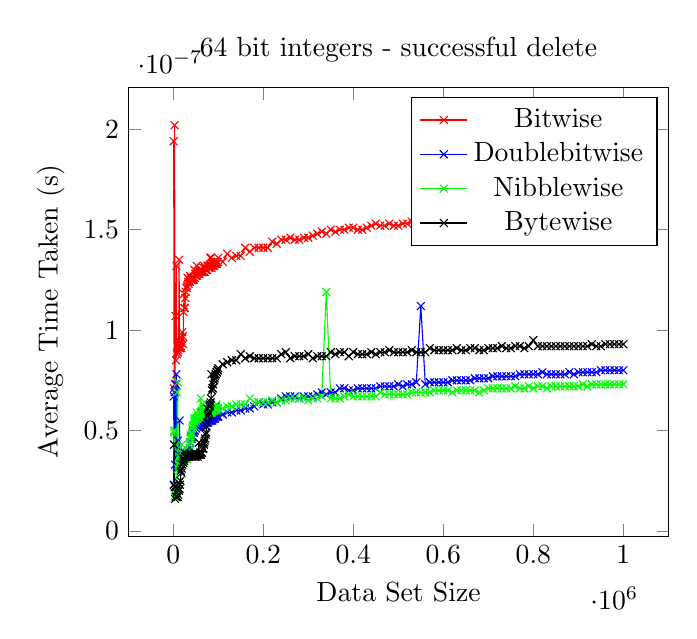
\begin{tikzpicture}
\begin{axis}[
xlabel=Data Set Size,
ylabel=Average Time Taken (s),
title=64 bit integers - successful delete]
\addplot[color=red,mark=x] coordinates {
(1000,0.000000194)
(2000,0.000000071)
(3000,0.000000202)
(4000,0.000000073)
(5000,0.000000107)
(6000,0.000000085)
(7000,0.000000132)
(8000,0.000000088)
(9000,0.000000089)
(10000,0.000000089)
(11000,0.00000009)
(12000,0.000000095)
(13000,0.000000135)
(14000,0.000000091)
(15000,0.000000091)
(16000,0.000000094)
(17000,0.000000092)
(18000,0.000000091)
(19000,0.000000096)
(20000,0.000000099)
(21000,0.000000097)
(22000,0.000000093)
(23000,0.000000109)
(24000,0.000000118)
(25000,0.000000111)
(26000,0.000000111)
(27000,0.000000116)
(28000,0.000000119)
(29000,0.000000121)
(30000,0.000000121)
(31000,0.000000122)
(32000,0.000000126)
(33000,0.000000124)
(34000,0.000000123)
(35000,0.000000125)
(36000,0.000000124)
(37000,0.000000124)
(38000,0.000000127)
(39000,0.000000126)
(40000,0.000000125)
(41000,0.000000125)
(42000,0.000000125)
(43000,0.000000125)
(44000,0.000000126)
(45000,0.000000126)
(46000,0.000000125)
(47000,0.00000013)
(48000,0.000000126)
(49000,0.000000128)
(50000,0.000000127)
(51000,0.000000127)
(52000,0.000000132)
(53000,0.000000127)
(54000,0.000000128)
(55000,0.000000128)
(56000,0.000000128)
(57000,0.000000129)
(58000,0.000000128)
(59000,0.000000129)
(60000,0.000000129)
(61000,0.000000129)
(62000,0.000000129)
(63000,0.00000013)
(64000,0.000000129)
(65000,0.000000129)
(66000,0.000000129)
(67000,0.000000131)
(68000,0.000000129)
(69000,0.000000132)
(70000,0.000000129)
(71000,0.000000131)
(72000,0.00000013)
(73000,0.00000013)
(74000,0.00000013)
(75000,0.00000013)
(76000,0.000000132)
(77000,0.000000132)
(78000,0.000000132)
(79000,0.000000131)
(80000,0.000000132)
(81000,0.000000131)
(82000,0.000000136)
(83000,0.000000132)
(84000,0.000000136)
(85000,0.000000131)
(86000,0.000000132)
(87000,0.000000132)
(88000,0.000000132)
(89000,0.000000133)
(90000,0.000000134)
(91000,0.000000132)
(92000,0.000000134)
(93000,0.000000133)
(94000,0.000000133)
(95000,0.000000133)
(96000,0.000000133)
(97000,0.000000133)
(98000,0.000000134)
(99000,0.000000134)
(100000,0.000000136)
(110000,0.000000134)
(120000,0.000000138)
(130000,0.000000136)
(140000,0.000000137)
(150000,0.000000137)
(160000,0.000000141)
(170000,0.000000139)
(180000,0.000000141)
(190000,0.000000141)
(200000,0.000000141)
(210000,0.000000141)
(220000,0.000000144)
(230000,0.000000143)
(240000,0.000000145)
(250000,0.000000145)
(260000,0.000000146)
(270000,0.000000145)
(280000,0.000000145)
(290000,0.000000146)
(300000,0.000000146)
(310000,0.000000147)
(320000,0.000000148)
(330000,0.000000149)
(340000,0.000000148)
(350000,0.00000015)
(360000,0.000000149)
(370000,0.00000015)
(380000,0.00000015)
(390000,0.000000151)
(400000,0.000000151)
(410000,0.00000015)
(420000,0.00000015)
(430000,0.000000151)
(440000,0.000000152)
(450000,0.000000153)
(460000,0.000000152)
(470000,0.000000152)
(480000,0.000000153)
(490000,0.000000152)
(500000,0.000000152)
(510000,0.000000153)
(520000,0.000000153)
(530000,0.000000154)
(540000,0.000000155)
(550000,0.000000155)
(560000,0.000000154)
(570000,0.000000155)
(580000,0.000000155)
(590000,0.000000155)
(600000,0.000000156)
(610000,0.000000155)
(620000,0.000000156)
(630000,0.000000156)
(640000,0.000000156)
(650000,0.000000157)
(660000,0.000000156)
(670000,0.000000157)
(680000,0.000000157)
(690000,0.000000157)
(700000,0.000000157)
(710000,0.000000158)
(720000,0.000000158)
(730000,0.000000158)
(740000,0.000000158)
(750000,0.000000159)
(760000,0.000000159)
(770000,0.000000159)
(780000,0.00000016)
(790000,0.000000159)
(800000,0.000000159)
(810000,0.00000016)
(820000,0.00000016)
(830000,0.00000016)
(840000,0.00000016)
(850000,0.000000161)
(860000,0.000000161)
(870000,0.000000164)
(880000,0.000000161)
(890000,0.000000161)
(900000,0.000000161)
(910000,0.000000162)
(920000,0.000000161)
(930000,0.000000162)
(940000,0.000000161)
(950000,0.000000162)
(960000,0.000000162)
(970000,0.000000162)
(980000,0.000000162)
(990000,0.000000162)
(1000000,0.000000162)
};
\addlegendentry{Bitwise}
\addplot[color=blue,mark=x] coordinates {
(1000,0.000000067)
(2000,0.000000023)
(3000,0.000000069)
(4000,0.000000033)
(5000,0.000000073)
(6000,0.000000073)
(7000,0.000000078)
(8000,0.000000032)
(9000,0.000000031)
(10000,0.000000045)
(11000,0.000000038)
(12000,0.000000038)
(13000,0.000000034)
(14000,0.000000055)
(15000,0.000000037)
(16000,0.000000035)
(17000,0.000000035)
(18000,0.000000039)
(19000,0.000000036)
(20000,0.000000035)
(21000,0.000000036)
(22000,0.000000036)
(23000,0.000000037)
(24000,0.000000036)
(25000,0.000000037)
(26000,0.000000038)
(27000,0.000000037)
(28000,0.000000037)
(29000,0.000000037)
(30000,0.000000039)
(31000,0.000000037)
(32000,0.000000037)
(33000,0.000000038)
(34000,0.00000004)
(35000,0.000000039)
(36000,0.00000004)
(37000,0.000000044)
(38000,0.000000041)
(39000,0.000000047)
(40000,0.000000046)
(41000,0.000000046)
(42000,0.000000047)
(43000,0.000000047)
(44000,0.00000005)
(45000,0.000000049)
(46000,0.000000049)
(47000,0.00000005)
(48000,0.00000005)
(49000,0.000000054)
(50000,0.000000053)
(51000,0.000000051)
(52000,0.000000052)
(53000,0.000000052)
(54000,0.000000052)
(55000,0.000000052)
(56000,0.000000052)
(57000,0.000000052)
(58000,0.000000052)
(59000,0.000000052)
(60000,0.000000053)
(61000,0.000000053)
(62000,0.000000053)
(63000,0.000000059)
(64000,0.000000053)
(65000,0.000000053)
(66000,0.000000054)
(67000,0.000000053)
(68000,0.000000054)
(69000,0.000000054)
(70000,0.000000056)
(71000,0.000000054)
(72000,0.000000054)
(73000,0.000000054)
(74000,0.000000054)
(75000,0.000000054)
(76000,0.000000054)
(77000,0.000000055)
(78000,0.000000054)
(79000,0.000000055)
(80000,0.000000055)
(81000,0.000000055)
(82000,0.000000055)
(83000,0.000000057)
(84000,0.000000055)
(85000,0.000000055)
(86000,0.000000056)
(87000,0.000000055)
(88000,0.000000056)
(89000,0.000000056)
(90000,0.000000056)
(91000,0.000000056)
(92000,0.000000057)
(93000,0.000000056)
(94000,0.000000062)
(95000,0.000000057)
(96000,0.000000057)
(97000,0.000000059)
(98000,0.000000057)
(99000,0.000000057)
(100000,0.000000057)
(110000,0.000000058)
(120000,0.000000059)
(130000,0.000000059)
(140000,0.00000006)
(150000,0.00000006)
(160000,0.000000061)
(170000,0.000000061)
(180000,0.000000062)
(190000,0.000000064)
(200000,0.000000063)
(210000,0.000000063)
(220000,0.000000064)
(230000,0.000000064)
(240000,0.000000066)
(250000,0.000000067)
(260000,0.000000067)
(270000,0.000000067)
(280000,0.000000066)
(290000,0.000000067)
(300000,0.000000067)
(310000,0.000000067)
(320000,0.000000068)
(330000,0.000000069)
(340000,0.000000068)
(350000,0.000000069)
(360000,0.000000069)
(370000,0.000000071)
(380000,0.000000071)
(390000,0.00000007)
(400000,0.00000007)
(410000,0.000000071)
(420000,0.000000071)
(430000,0.000000071)
(440000,0.000000071)
(450000,0.000000071)
(460000,0.000000072)
(470000,0.000000072)
(480000,0.000000072)
(490000,0.000000072)
(500000,0.000000073)
(510000,0.000000072)
(520000,0.000000073)
(530000,0.000000073)
(540000,0.000000074)
(550000,0.000000112)
(560000,0.000000073)
(570000,0.000000074)
(580000,0.000000074)
(590000,0.000000074)
(600000,0.000000074)
(610000,0.000000074)
(620000,0.000000075)
(630000,0.000000075)
(640000,0.000000075)
(650000,0.000000075)
(660000,0.000000075)
(670000,0.000000076)
(680000,0.000000076)
(690000,0.000000076)
(700000,0.000000076)
(710000,0.000000077)
(720000,0.000000077)
(730000,0.000000077)
(740000,0.000000077)
(750000,0.000000077)
(760000,0.000000077)
(770000,0.000000078)
(780000,0.000000078)
(790000,0.000000078)
(800000,0.000000078)
(810000,0.000000078)
(820000,0.000000079)
(830000,0.000000078)
(840000,0.000000078)
(850000,0.000000078)
(860000,0.000000078)
(870000,0.000000078)
(880000,0.000000079)
(890000,0.000000078)
(900000,0.000000079)
(910000,0.000000079)
(920000,0.000000079)
(930000,0.000000079)
(940000,0.000000079)
(950000,0.00000008)
(960000,0.00000008)
(970000,0.00000008)
(980000,0.00000008)
(990000,0.00000008)
(1000000,0.00000008)
};
\addlegendentry{Doublebitwise}
\addplot[color=green,mark=x] coordinates {
(1000,0.000000049)
(2000,0.00000005)
(3000,0.00000005)
(4000,0.000000017)
(5000,0.000000018)
(6000,0.000000018)
(7000,0.000000019)
(8000,0.000000022)
(9000,0.000000069)
(10000,0.000000074)
(11000,0.000000031)
(12000,0.000000033)
(13000,0.000000037)
(14000,0.000000033)
(15000,0.000000034)
(16000,0.000000035)
(17000,0.000000035)
(18000,0.000000039)
(19000,0.000000043)
(20000,0.000000035)
(21000,0.000000036)
(22000,0.000000035)
(23000,0.000000034)
(24000,0.000000035)
(25000,0.000000035)
(26000,0.000000038)
(27000,0.000000037)
(28000,0.000000036)
(29000,0.000000036)
(30000,0.000000036)
(31000,0.000000036)
(32000,0.000000037)
(33000,0.000000038)
(34000,0.00000004)
(35000,0.00000004)
(36000,0.000000043)
(37000,0.000000044)
(38000,0.000000046)
(39000,0.000000047)
(40000,0.000000048)
(41000,0.000000049)
(42000,0.000000051)
(43000,0.000000052)
(44000,0.000000052)
(45000,0.000000053)
(46000,0.000000055)
(47000,0.000000056)
(48000,0.000000054)
(49000,0.000000056)
(50000,0.000000055)
(51000,0.000000056)
(52000,0.000000059)
(53000,0.000000056)
(54000,0.000000056)
(55000,0.000000057)
(56000,0.000000057)
(57000,0.000000057)
(58000,0.000000057)
(59000,0.000000057)
(60000,0.000000059)
(61000,0.000000066)
(62000,0.000000058)
(63000,0.00000006)
(64000,0.000000058)
(65000,0.000000063)
(66000,0.000000058)
(67000,0.000000061)
(68000,0.000000059)
(69000,0.000000058)
(70000,0.000000059)
(71000,0.00000006)
(72000,0.000000059)
(73000,0.000000059)
(74000,0.000000058)
(75000,0.000000058)
(76000,0.000000058)
(77000,0.000000059)
(78000,0.000000059)
(79000,0.000000059)
(80000,0.000000059)
(81000,0.000000059)
(82000,0.000000059)
(83000,0.000000059)
(84000,0.000000059)
(85000,0.00000006)
(86000,0.000000059)
(87000,0.00000006)
(88000,0.00000006)
(89000,0.00000006)
(90000,0.00000006)
(91000,0.000000061)
(92000,0.000000061)
(93000,0.000000061)
(94000,0.00000006)
(95000,0.000000061)
(96000,0.000000063)
(97000,0.00000006)
(98000,0.000000061)
(99000,0.000000061)
(100000,0.000000061)
(110000,0.000000061)
(120000,0.000000062)
(130000,0.000000062)
(140000,0.000000063)
(150000,0.000000063)
(160000,0.000000063)
(170000,0.000000066)
(180000,0.000000064)
(190000,0.000000064)
(200000,0.000000064)
(210000,0.000000064)
(220000,0.000000065)
(230000,0.000000064)
(240000,0.000000065)
(250000,0.000000065)
(260000,0.000000066)
(270000,0.000000066)
(280000,0.000000066)
(290000,0.000000066)
(300000,0.000000065)
(310000,0.000000066)
(320000,0.000000066)
(330000,0.000000067)
(340000,0.000000119)
(350000,0.000000066)
(360000,0.000000066)
(370000,0.000000066)
(380000,0.000000067)
(390000,0.000000068)
(400000,0.000000067)
(410000,0.000000067)
(420000,0.000000067)
(430000,0.000000067)
(440000,0.000000067)
(450000,0.000000067)
(460000,0.000000069)
(470000,0.000000068)
(480000,0.000000068)
(490000,0.000000068)
(500000,0.000000068)
(510000,0.000000068)
(520000,0.000000068)
(530000,0.000000069)
(540000,0.000000069)
(550000,0.000000069)
(560000,0.000000069)
(570000,0.000000069)
(580000,0.00000007)
(590000,0.00000007)
(600000,0.00000007)
(610000,0.00000007)
(620000,0.000000069)
(630000,0.00000007)
(640000,0.00000007)
(650000,0.00000007)
(660000,0.00000007)
(670000,0.00000007)
(680000,0.000000069)
(690000,0.00000007)
(700000,0.000000071)
(710000,0.000000071)
(720000,0.000000071)
(730000,0.000000071)
(740000,0.000000071)
(750000,0.000000071)
(760000,0.000000072)
(770000,0.000000071)
(780000,0.000000071)
(790000,0.000000072)
(800000,0.000000071)
(810000,0.000000072)
(820000,0.000000072)
(830000,0.000000071)
(840000,0.000000072)
(850000,0.000000072)
(860000,0.000000072)
(870000,0.000000072)
(880000,0.000000072)
(890000,0.000000072)
(900000,0.000000072)
(910000,0.000000073)
(920000,0.000000072)
(930000,0.000000073)
(940000,0.000000073)
(950000,0.000000073)
(960000,0.000000073)
(970000,0.000000073)
(980000,0.000000073)
(990000,0.000000073)
(1000000,0.000000073)
};
\addlegendentry{Nibblewise}
\addplot[color=black,mark=x] coordinates {
(1000,0.000000023)
(2000,0.000000043)
(3000,0.000000022)
(4000,0.000000016)
(5000,0.000000022)
(6000,0.000000017)
(7000,0.000000017)
(8000,0.000000019)
(9000,0.000000017)
(10000,0.000000017)
(11000,0.000000018)
(12000,0.000000024)
(13000,0.00000002)
(14000,0.000000021)
(15000,0.000000023)
(16000,0.000000025)
(17000,0.00000003)
(18000,0.000000029)
(19000,0.000000031)
(20000,0.000000033)
(21000,0.000000036)
(22000,0.000000034)
(23000,0.000000035)
(24000,0.000000036)
(25000,0.000000039)
(26000,0.000000037)
(27000,0.000000037)
(28000,0.000000037)
(29000,0.000000037)
(30000,0.000000037)
(31000,0.000000038)
(32000,0.000000037)
(33000,0.000000037)
(34000,0.000000037)
(35000,0.000000037)
(36000,0.000000038)
(37000,0.000000038)
(38000,0.000000037)
(39000,0.000000038)
(40000,0.000000038)
(41000,0.000000038)
(42000,0.000000037)
(43000,0.000000038)
(44000,0.000000038)
(45000,0.000000037)
(46000,0.000000038)
(47000,0.000000039)
(48000,0.000000037)
(49000,0.000000038)
(50000,0.000000037)
(51000,0.000000038)
(52000,0.000000038)
(53000,0.000000038)
(54000,0.000000037)
(55000,0.000000038)
(56000,0.000000038)
(57000,0.000000044)
(58000,0.000000038)
(59000,0.000000038)
(60000,0.000000039)
(61000,0.000000038)
(62000,0.000000038)
(63000,0.000000039)
(64000,0.000000039)
(65000,0.000000041)
(66000,0.000000041)
(67000,0.000000041)
(68000,0.000000043)
(69000,0.000000044)
(70000,0.000000045)
(71000,0.000000046)
(72000,0.000000048)
(73000,0.000000049)
(74000,0.000000052)
(75000,0.000000054)
(76000,0.000000061)
(77000,0.000000057)
(78000,0.000000058)
(79000,0.000000059)
(80000,0.000000062)
(81000,0.000000062)
(82000,0.000000063)
(83000,0.000000064)
(84000,0.000000066)
(85000,0.000000078)
(86000,0.00000007)
(87000,0.000000071)
(88000,0.000000071)
(89000,0.000000073)
(90000,0.000000075)
(91000,0.000000075)
(92000,0.000000076)
(93000,0.000000077)
(94000,0.000000078)
(95000,0.000000078)
(96000,0.000000079)
(97000,0.000000079)
(98000,0.00000008)
(99000,0.00000008)
(100000,0.000000081)
(110000,0.000000083)
(120000,0.000000084)
(130000,0.000000085)
(140000,0.000000085)
(150000,0.000000088)
(160000,0.000000086)
(170000,0.000000087)
(180000,0.000000086)
(190000,0.000000086)
(200000,0.000000086)
(210000,0.000000086)
(220000,0.000000086)
(230000,0.000000086)
(240000,0.000000088)
(250000,0.000000089)
(260000,0.000000086)
(270000,0.000000087)
(280000,0.000000087)
(290000,0.000000087)
(300000,0.000000088)
(310000,0.000000086)
(320000,0.000000087)
(330000,0.000000087)
(340000,0.000000087)
(350000,0.000000089)
(360000,0.000000088)
(370000,0.000000089)
(380000,0.000000089)
(390000,0.000000087)
(400000,0.000000089)
(410000,0.000000088)
(420000,0.000000088)
(430000,0.000000088)
(440000,0.000000089)
(450000,0.000000088)
(460000,0.000000089)
(470000,0.000000089)
(480000,0.00000009)
(490000,0.000000089)
(500000,0.000000089)
(510000,0.000000089)
(520000,0.000000089)
(530000,0.00000009)
(540000,0.000000089)
(550000,0.000000089)
(560000,0.000000089)
(570000,0.000000091)
(580000,0.00000009)
(590000,0.00000009)
(600000,0.00000009)
(610000,0.00000009)
(620000,0.00000009)
(630000,0.000000091)
(640000,0.00000009)
(650000,0.00000009)
(660000,0.000000091)
(670000,0.000000091)
(680000,0.00000009)
(690000,0.00000009)
(700000,0.000000091)
(710000,0.000000091)
(720000,0.000000091)
(730000,0.000000092)
(740000,0.000000091)
(750000,0.000000091)
(760000,0.000000092)
(770000,0.000000092)
(780000,0.000000091)
(790000,0.000000092)
(800000,0.000000095)
(810000,0.000000092)
(820000,0.000000092)
(830000,0.000000092)
(840000,0.000000092)
(850000,0.000000092)
(860000,0.000000092)
(870000,0.000000092)
(880000,0.000000092)
(890000,0.000000092)
(900000,0.000000092)
(910000,0.000000092)
(920000,0.000000092)
(930000,0.000000093)
(940000,0.000000092)
(950000,0.000000092)
(960000,0.000000093)
(970000,0.000000093)
(980000,0.000000093)
(990000,0.000000093)
(1000000,0.000000093)
};
\addlegendentry{Bytewise}
\end{axis}
\end{tikzpicture}

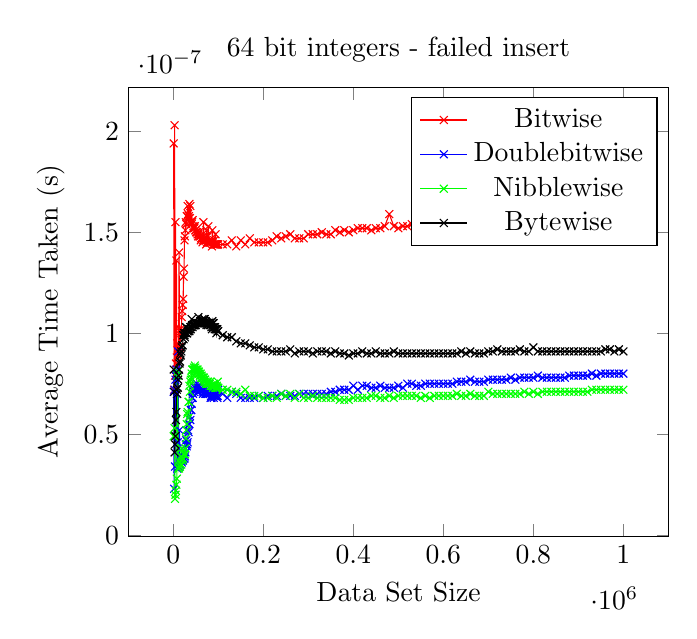
\begin{tikzpicture}
\begin{axis}[
xlabel=Data Set Size,
ylabel=Average Time Taken (s),
title=64 bit integers - failed insert]
\addplot[color=red,mark=x] coordinates {
(1000,0.000000194)
(2000,0.000000072)
(3000,0.000000203)
(4000,0.000000079)
(5000,0.000000155)
(6000,0.000000085)
(7000,0.000000136)
(8000,0.000000088)
(9000,0.000000095)
(10000,0.000000089)
(11000,0.00000009)
(12000,0.000000091)
(13000,0.00000014)
(14000,0.000000093)
(15000,0.000000093)
(16000,0.000000102)
(17000,0.000000101)
(18000,0.0000001)
(19000,0.000000108)
(20000,0.000000111)
(21000,0.000000114)
(22000,0.000000117)
(23000,0.000000128)
(24000,0.000000132)
(25000,0.000000146)
(26000,0.000000148)
(27000,0.000000151)
(28000,0.000000155)
(29000,0.000000154)
(30000,0.000000158)
(31000,0.000000158)
(32000,0.000000163)
(33000,0.000000159)
(34000,0.000000157)
(35000,0.000000158)
(36000,0.000000164)
(37000,0.000000157)
(38000,0.000000163)
(39000,0.000000155)
(40000,0.000000155)
(41000,0.000000154)
(42000,0.000000155)
(43000,0.000000156)
(44000,0.000000152)
(45000,0.000000153)
(46000,0.000000152)
(47000,0.000000152)
(48000,0.000000153)
(49000,0.000000151)
(50000,0.000000151)
(51000,0.00000015)
(52000,0.00000015)
(53000,0.00000015)
(54000,0.000000149)
(55000,0.000000148)
(56000,0.000000149)
(57000,0.00000015)
(58000,0.000000148)
(59000,0.000000148)
(60000,0.000000148)
(61000,0.000000146)
(62000,0.000000147)
(63000,0.000000147)
(64000,0.000000147)
(65000,0.000000145)
(66000,0.000000146)
(67000,0.000000155)
(68000,0.000000147)
(69000,0.000000146)
(70000,0.000000146)
(71000,0.000000147)
(72000,0.000000146)
(73000,0.000000144)
(74000,0.000000151)
(75000,0.000000145)
(76000,0.000000145)
(77000,0.000000148)
(78000,0.000000153)
(79000,0.000000145)
(80000,0.000000145)
(81000,0.000000145)
(82000,0.000000145)
(83000,0.000000145)
(84000,0.000000145)
(85000,0.000000146)
(86000,0.000000143)
(87000,0.000000151)
(88000,0.000000145)
(89000,0.000000144)
(90000,0.000000144)
(91000,0.000000146)
(92000,0.000000144)
(93000,0.000000144)
(94000,0.000000149)
(95000,0.000000144)
(96000,0.000000144)
(97000,0.000000144)
(98000,0.000000144)
(99000,0.000000144)
(100000,0.000000144)
(110000,0.000000144)
(120000,0.000000144)
(130000,0.000000146)
(140000,0.000000143)
(150000,0.000000146)
(160000,0.000000144)
(170000,0.000000147)
(180000,0.000000145)
(190000,0.000000145)
(200000,0.000000145)
(210000,0.000000145)
(220000,0.000000146)
(230000,0.000000148)
(240000,0.000000147)
(250000,0.000000148)
(260000,0.000000149)
(270000,0.000000147)
(280000,0.000000147)
(290000,0.000000147)
(300000,0.000000149)
(310000,0.000000149)
(320000,0.000000149)
(330000,0.00000015)
(340000,0.000000149)
(350000,0.000000149)
(360000,0.000000151)
(370000,0.00000015)
(380000,0.000000151)
(390000,0.00000015)
(400000,0.000000151)
(410000,0.000000152)
(420000,0.000000152)
(430000,0.000000152)
(440000,0.000000151)
(450000,0.000000152)
(460000,0.000000152)
(470000,0.000000153)
(480000,0.000000159)
(490000,0.000000153)
(500000,0.000000152)
(510000,0.000000153)
(520000,0.000000153)
(530000,0.000000154)
(540000,0.000000153)
(550000,0.000000154)
(560000,0.000000154)
(570000,0.000000155)
(580000,0.000000155)
(590000,0.000000155)
(600000,0.000000155)
(610000,0.000000156)
(620000,0.000000155)
(630000,0.000000156)
(640000,0.000000156)
(650000,0.000000156)
(660000,0.000000156)
(670000,0.000000156)
(680000,0.000000157)
(690000,0.000000157)
(700000,0.000000157)
(710000,0.000000157)
(720000,0.000000157)
(730000,0.000000157)
(740000,0.000000158)
(750000,0.000000158)
(760000,0.000000157)
(770000,0.000000158)
(780000,0.000000159)
(790000,0.000000158)
(800000,0.000000158)
(810000,0.000000159)
(820000,0.000000159)
(830000,0.000000159)
(840000,0.00000016)
(850000,0.00000016)
(860000,0.000000159)
(870000,0.000000159)
(880000,0.00000016)
(890000,0.00000016)
(900000,0.000000163)
(910000,0.00000016)
(920000,0.00000016)
(930000,0.00000016)
(940000,0.00000016)
(950000,0.000000161)
(960000,0.00000016)
(970000,0.00000016)
(980000,0.000000161)
(990000,0.000000161)
(1000000,0.000000161)
};
\addlegendentry{Bitwise}
\addplot[color=blue,mark=x] coordinates {
(1000,0.000000071)
(2000,0.000000023)
(3000,0.000000072)
(4000,0.000000034)
(5000,0.000000077)
(6000,0.000000079)
(7000,0.000000082)
(8000,0.00000007)
(9000,0.000000033)
(10000,0.000000046)
(11000,0.000000091)
(12000,0.000000034)
(13000,0.000000034)
(14000,0.000000052)
(15000,0.000000035)
(16000,0.000000039)
(17000,0.000000037)
(18000,0.000000037)
(19000,0.000000036)
(20000,0.000000038)
(21000,0.000000037)
(22000,0.000000037)
(23000,0.000000038)
(24000,0.000000038)
(25000,0.000000038)
(26000,0.000000039)
(27000,0.000000041)
(28000,0.000000045)
(29000,0.000000047)
(30000,0.000000044)
(31000,0.000000045)
(32000,0.000000046)
(33000,0.000000052)
(34000,0.000000051)
(35000,0.000000055)
(36000,0.000000055)
(37000,0.000000059)
(38000,0.000000057)
(39000,0.000000062)
(40000,0.000000062)
(41000,0.000000065)
(42000,0.000000068)
(43000,0.000000068)
(44000,0.00000007)
(45000,0.000000072)
(46000,0.000000071)
(47000,0.000000072)
(48000,0.000000073)
(49000,0.000000073)
(50000,0.000000073)
(51000,0.000000073)
(52000,0.000000075)
(53000,0.000000073)
(54000,0.000000073)
(55000,0.000000071)
(56000,0.000000071)
(57000,0.000000074)
(58000,0.000000073)
(59000,0.000000072)
(60000,0.000000072)
(61000,0.000000072)
(62000,0.000000072)
(63000,0.000000072)
(64000,0.000000072)
(65000,0.000000071)
(66000,0.00000007)
(67000,0.000000072)
(68000,0.000000074)
(69000,0.000000071)
(70000,0.000000071)
(71000,0.00000007)
(72000,0.000000071)
(73000,0.00000007)
(74000,0.000000071)
(75000,0.00000007)
(76000,0.00000007)
(77000,0.00000007)
(78000,0.00000007)
(79000,0.000000072)
(80000,0.000000075)
(81000,0.00000007)
(82000,0.00000007)
(83000,0.000000068)
(84000,0.000000069)
(85000,0.000000068)
(86000,0.000000069)
(87000,0.000000069)
(88000,0.000000072)
(89000,0.00000007)
(90000,0.000000068)
(91000,0.000000069)
(92000,0.00000007)
(93000,0.000000069)
(94000,0.000000069)
(95000,0.000000069)
(96000,0.000000073)
(97000,0.000000069)
(98000,0.000000068)
(99000,0.000000069)
(100000,0.000000072)
(110000,0.00000007)
(120000,0.000000068)
(130000,0.000000071)
(140000,0.00000007)
(150000,0.000000068)
(160000,0.000000068)
(170000,0.000000068)
(180000,0.000000068)
(190000,0.000000069)
(200000,0.000000068)
(210000,0.000000069)
(220000,0.000000069)
(230000,0.000000069)
(240000,0.00000007)
(250000,0.000000069)
(260000,0.000000069)
(270000,0.000000069)
(280000,0.00000007)
(290000,0.00000007)
(300000,0.00000007)
(310000,0.00000007)
(320000,0.00000007)
(330000,0.00000007)
(340000,0.00000007)
(350000,0.000000071)
(360000,0.000000071)
(370000,0.000000072)
(380000,0.000000072)
(390000,0.000000072)
(400000,0.000000074)
(410000,0.000000072)
(420000,0.000000074)
(430000,0.000000074)
(440000,0.000000073)
(450000,0.000000073)
(460000,0.000000074)
(470000,0.000000073)
(480000,0.000000073)
(490000,0.000000073)
(500000,0.000000074)
(510000,0.000000073)
(520000,0.000000075)
(530000,0.000000075)
(540000,0.000000074)
(550000,0.000000074)
(560000,0.000000075)
(570000,0.000000075)
(580000,0.000000075)
(590000,0.000000075)
(600000,0.000000075)
(610000,0.000000075)
(620000,0.000000075)
(630000,0.000000076)
(640000,0.000000076)
(650000,0.000000076)
(660000,0.000000077)
(670000,0.000000076)
(680000,0.000000076)
(690000,0.000000076)
(700000,0.000000077)
(710000,0.000000077)
(720000,0.000000077)
(730000,0.000000077)
(740000,0.000000077)
(750000,0.000000078)
(760000,0.000000077)
(770000,0.000000078)
(780000,0.000000078)
(790000,0.000000078)
(800000,0.000000078)
(810000,0.000000079)
(820000,0.000000078)
(830000,0.000000078)
(840000,0.000000078)
(850000,0.000000078)
(860000,0.000000078)
(870000,0.000000078)
(880000,0.000000079)
(890000,0.000000079)
(900000,0.000000079)
(910000,0.000000079)
(920000,0.000000079)
(930000,0.00000008)
(940000,0.000000079)
(950000,0.00000008)
(960000,0.00000008)
(970000,0.00000008)
(980000,0.00000008)
(990000,0.00000008)
(1000000,0.00000008)
};
\addlegendentry{Doublebitwise}
\addplot[color=green,mark=x] coordinates {
(1000,0.000000049)
(2000,0.000000049)
(3000,0.000000053)
(4000,0.000000018)
(5000,0.00000002)
(6000,0.000000022)
(7000,0.000000025)
(8000,0.000000028)
(9000,0.000000079)
(10000,0.000000081)
(11000,0.000000033)
(12000,0.000000037)
(13000,0.000000033)
(14000,0.000000034)
(15000,0.000000034)
(16000,0.000000035)
(17000,0.000000039)
(18000,0.000000035)
(19000,0.000000043)
(20000,0.000000037)
(21000,0.000000038)
(22000,0.000000038)
(23000,0.000000042)
(24000,0.00000004)
(25000,0.00000004)
(26000,0.00000004)
(27000,0.000000043)
(28000,0.000000048)
(29000,0.000000052)
(30000,0.000000055)
(31000,0.00000006)
(32000,0.000000061)
(33000,0.000000058)
(34000,0.000000066)
(35000,0.000000066)
(36000,0.000000074)
(37000,0.000000071)
(38000,0.000000076)
(39000,0.000000077)
(40000,0.000000078)
(41000,0.00000008)
(42000,0.000000082)
(43000,0.000000082)
(44000,0.000000082)
(45000,0.000000082)
(46000,0.000000083)
(47000,0.000000082)
(48000,0.000000084)
(49000,0.000000083)
(50000,0.000000082)
(51000,0.000000081)
(52000,0.000000082)
(53000,0.000000081)
(54000,0.000000082)
(55000,0.000000081)
(56000,0.00000008)
(57000,0.000000081)
(58000,0.00000008)
(59000,0.000000079)
(60000,0.000000079)
(61000,0.00000008)
(62000,0.000000078)
(63000,0.000000079)
(64000,0.000000078)
(65000,0.000000078)
(66000,0.000000078)
(67000,0.000000077)
(68000,0.000000078)
(69000,0.000000076)
(70000,0.000000077)
(71000,0.000000077)
(72000,0.000000076)
(73000,0.000000075)
(74000,0.000000075)
(75000,0.000000075)
(76000,0.000000076)
(77000,0.000000076)
(78000,0.000000075)
(79000,0.000000075)
(80000,0.000000075)
(81000,0.000000075)
(82000,0.000000076)
(83000,0.000000074)
(84000,0.000000074)
(85000,0.000000074)
(86000,0.000000074)
(87000,0.000000074)
(88000,0.000000073)
(89000,0.000000074)
(90000,0.000000074)
(91000,0.000000075)
(92000,0.000000074)
(93000,0.000000073)
(94000,0.000000073)
(95000,0.000000073)
(96000,0.000000073)
(97000,0.000000074)
(98000,0.000000073)
(99000,0.000000076)
(100000,0.000000073)
(110000,0.000000072)
(120000,0.000000072)
(130000,0.000000071)
(140000,0.000000071)
(150000,0.00000007)
(160000,0.000000072)
(170000,0.000000069)
(180000,0.000000069)
(190000,0.000000069)
(200000,0.000000068)
(210000,0.000000068)
(220000,0.000000069)
(230000,0.000000068)
(240000,0.00000007)
(250000,0.000000069)
(260000,0.00000007)
(270000,0.000000068)
(280000,0.00000007)
(290000,0.000000068)
(300000,0.000000068)
(310000,0.000000069)
(320000,0.000000068)
(330000,0.000000068)
(340000,0.000000068)
(350000,0.000000068)
(360000,0.000000068)
(370000,0.000000067)
(380000,0.000000067)
(390000,0.000000067)
(400000,0.000000068)
(410000,0.000000068)
(420000,0.000000068)
(430000,0.000000068)
(440000,0.000000069)
(450000,0.000000069)
(460000,0.000000068)
(470000,0.000000068)
(480000,0.000000069)
(490000,0.000000068)
(500000,0.000000069)
(510000,0.000000069)
(520000,0.000000069)
(530000,0.000000069)
(540000,0.000000069)
(550000,0.000000068)
(560000,0.000000069)
(570000,0.000000068)
(580000,0.000000069)
(590000,0.000000069)
(600000,0.000000069)
(610000,0.000000069)
(620000,0.000000069)
(630000,0.00000007)
(640000,0.000000069)
(650000,0.000000069)
(660000,0.00000007)
(670000,0.000000069)
(680000,0.000000069)
(690000,0.000000069)
(700000,0.000000071)
(710000,0.00000007)
(720000,0.00000007)
(730000,0.00000007)
(740000,0.00000007)
(750000,0.00000007)
(760000,0.00000007)
(770000,0.00000007)
(780000,0.000000071)
(790000,0.00000007)
(800000,0.000000071)
(810000,0.00000007)
(820000,0.000000071)
(830000,0.000000071)
(840000,0.000000071)
(850000,0.000000071)
(860000,0.000000071)
(870000,0.000000071)
(880000,0.000000071)
(890000,0.000000071)
(900000,0.000000071)
(910000,0.000000071)
(920000,0.000000071)
(930000,0.000000072)
(940000,0.000000072)
(950000,0.000000072)
(960000,0.000000072)
(970000,0.000000072)
(980000,0.000000072)
(990000,0.000000072)
(1000000,0.000000072)
};
\addlegendentry{Nibblewise}
\addplot[color=black,mark=x] coordinates {
(1000,0.000000082)
(2000,0.000000071)
(3000,0.000000041)
(4000,0.000000045)
(5000,0.000000049)
(6000,0.000000057)
(7000,0.000000061)
(8000,0.000000072)
(9000,0.00000007)
(10000,0.000000073)
(11000,0.000000077)
(12000,0.000000079)
(13000,0.000000082)
(14000,0.000000085)
(15000,0.000000086)
(16000,0.00000009)
(17000,0.000000089)
(18000,0.000000091)
(19000,0.000000093)
(20000,0.000000094)
(21000,0.000000094)
(22000,0.000000099)
(23000,0.000000097)
(24000,0.0000001)
(25000,0.000000099)
(26000,0.000000098)
(27000,0.0000001)
(28000,0.000000103)
(29000,0.000000103)
(30000,0.0000001)
(31000,0.0000001)
(32000,0.000000101)
(33000,0.000000101)
(34000,0.000000102)
(35000,0.000000102)
(36000,0.000000101)
(37000,0.000000102)
(38000,0.000000103)
(39000,0.000000102)
(40000,0.000000103)
(41000,0.000000107)
(42000,0.000000104)
(43000,0.000000103)
(44000,0.000000104)
(45000,0.000000104)
(46000,0.000000104)
(47000,0.000000104)
(48000,0.000000104)
(49000,0.000000105)
(50000,0.000000104)
(51000,0.000000105)
(52000,0.000000105)
(53000,0.000000105)
(54000,0.000000105)
(55000,0.000000105)
(56000,0.000000108)
(57000,0.000000105)
(58000,0.000000105)
(59000,0.000000105)
(60000,0.000000106)
(61000,0.000000106)
(62000,0.000000106)
(63000,0.000000105)
(64000,0.000000106)
(65000,0.000000107)
(66000,0.000000106)
(67000,0.000000105)
(68000,0.000000106)
(69000,0.000000107)
(70000,0.000000107)
(71000,0.000000105)
(72000,0.000000106)
(73000,0.000000105)
(74000,0.000000104)
(75000,0.000000105)
(76000,0.000000105)
(77000,0.000000104)
(78000,0.000000105)
(79000,0.000000105)
(80000,0.000000105)
(81000,0.000000104)
(82000,0.000000105)
(83000,0.000000104)
(84000,0.000000104)
(85000,0.000000103)
(86000,0.000000102)
(87000,0.000000106)
(88000,0.000000105)
(89000,0.000000103)
(90000,0.000000105)
(91000,0.000000103)
(92000,0.000000102)
(93000,0.000000103)
(94000,0.000000102)
(95000,0.000000102)
(96000,0.0000001)
(97000,0.000000102)
(98000,0.000000102)
(99000,0.000000101)
(100000,0.000000101)
(110000,0.000000099)
(120000,0.000000098)
(130000,0.000000098)
(140000,0.000000096)
(150000,0.000000095)
(160000,0.000000095)
(170000,0.000000094)
(180000,0.000000093)
(190000,0.000000093)
(200000,0.000000092)
(210000,0.000000092)
(220000,0.000000091)
(230000,0.000000091)
(240000,0.000000091)
(250000,0.000000091)
(260000,0.000000092)
(270000,0.00000009)
(280000,0.000000091)
(290000,0.000000091)
(300000,0.000000091)
(310000,0.00000009)
(320000,0.000000091)
(330000,0.000000091)
(340000,0.000000091)
(350000,0.00000009)
(360000,0.000000091)
(370000,0.00000009)
(380000,0.00000009)
(390000,0.000000089)
(400000,0.00000009)
(410000,0.00000009)
(420000,0.000000091)
(430000,0.00000009)
(440000,0.00000009)
(450000,0.000000091)
(460000,0.00000009)
(470000,0.00000009)
(480000,0.00000009)
(490000,0.000000091)
(500000,0.00000009)
(510000,0.00000009)
(520000,0.00000009)
(530000,0.00000009)
(540000,0.00000009)
(550000,0.00000009)
(560000,0.00000009)
(570000,0.00000009)
(580000,0.00000009)
(590000,0.00000009)
(600000,0.00000009)
(610000,0.00000009)
(620000,0.00000009)
(630000,0.00000009)
(640000,0.000000091)
(650000,0.00000009)
(660000,0.000000091)
(670000,0.00000009)
(680000,0.00000009)
(690000,0.00000009)
(700000,0.000000091)
(710000,0.000000091)
(720000,0.000000092)
(730000,0.000000091)
(740000,0.000000091)
(750000,0.000000091)
(760000,0.000000091)
(770000,0.000000092)
(780000,0.000000091)
(790000,0.000000091)
(800000,0.000000093)
(810000,0.000000091)
(820000,0.000000091)
(830000,0.000000091)
(840000,0.000000091)
(850000,0.000000091)
(860000,0.000000091)
(870000,0.000000091)
(880000,0.000000091)
(890000,0.000000091)
(900000,0.000000091)
(910000,0.000000091)
(920000,0.000000091)
(930000,0.000000091)
(940000,0.000000091)
(950000,0.000000091)
(960000,0.000000092)
(970000,0.000000092)
(980000,0.000000091)
(990000,0.000000092)
(1000000,0.000000091)
};
\addlegendentry{Bytewise}
\end{axis}
\end{tikzpicture}

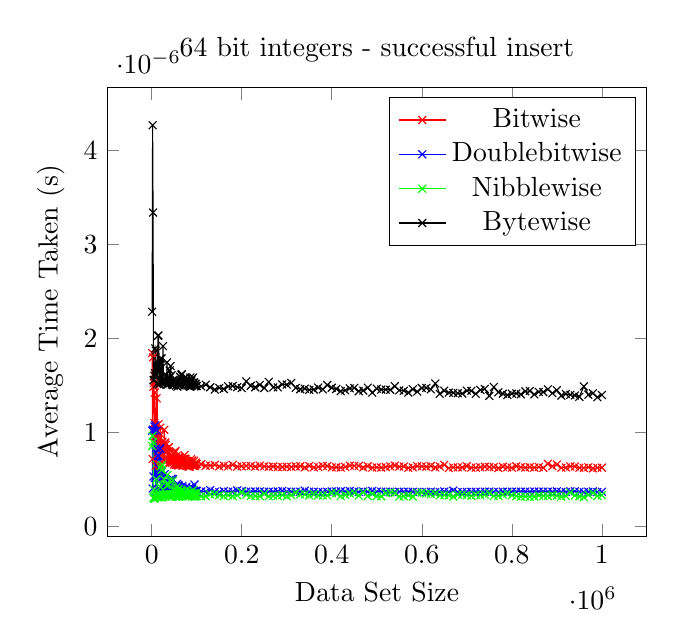
\begin{tikzpicture}
\begin{axis}[
xlabel=Data Set Size,
ylabel=Average Time Taken (s),
title=64 bit integers - successful insert]
\addplot[color=red,mark=x] coordinates {
(1000,0.000001843)
(2000,0.000000716)
(3000,0.000001798)
(4000,0.000001485)
(5000,0.000001525)
(6000,0.000001098)
(7000,0.000001423)
(8000,0.000000957)
(9000,0.000000642)
(10000,0.000000932)
(11000,0.000001362)
(12000,0.000001511)
(13000,0.000000805)
(14000,0.000000877)
(15000,0.000001086)
(16000,0.000000666)
(17000,0.000000646)
(18000,0.000000638)
(19000,0.00000105)
(20000,0.000000757)
(21000,0.000000974)
(22000,0.00000077)
(23000,0.00000089)
(24000,0.0000009)
(25000,0.000000835)
(26000,0.000000807)
(27000,0.000000704)
(28000,0.000001026)
(29000,0.000000881)
(30000,0.000000893)
(31000,0.000000866)
(32000,0.000000821)
(33000,0.000000791)
(34000,0.000000798)
(35000,0.000000702)
(36000,0.000000725)
(37000,0.000000835)
(38000,0.000000843)
(39000,0.00000068)
(40000,0.000000707)
(41000,0.000000676)
(42000,0.00000074)
(43000,0.000000725)
(44000,0.000000761)
(45000,0.000000676)
(46000,0.000000712)
(47000,0.000000681)
(48000,0.00000077)
(49000,0.000000779)
(50000,0.000000657)
(51000,0.000000662)
(52000,0.00000079)
(53000,0.000000802)
(54000,0.000000654)
(55000,0.000000747)
(56000,0.000000654)
(57000,0.000000678)
(58000,0.000000648)
(59000,0.000000654)
(60000,0.000000734)
(61000,0.000000649)
(62000,0.00000073)
(63000,0.000000666)
(64000,0.000000706)
(65000,0.000000674)
(66000,0.000000662)
(67000,0.000000673)
(68000,0.000000649)
(69000,0.000000645)
(70000,0.000000717)
(71000,0.000000711)
(72000,0.000000717)
(73000,0.000000757)
(74000,0.000000675)
(75000,0.000000718)
(76000,0.000000653)
(77000,0.000000686)
(78000,0.000000643)
(79000,0.000000643)
(80000,0.000000648)
(81000,0.000000687)
(82000,0.000000633)
(83000,0.000000652)
(84000,0.000000634)
(85000,0.000000661)
(86000,0.000000663)
(87000,0.000000714)
(88000,0.000000669)
(89000,0.000000649)
(90000,0.000000701)
(91000,0.000000653)
(92000,0.000000683)
(93000,0.000000642)
(94000,0.000000697)
(95000,0.000000641)
(96000,0.000000646)
(97000,0.000000656)
(98000,0.000000678)
(99000,0.000000665)
(100000,0.000000664)
(110000,0.00000066)
(120000,0.000000644)
(130000,0.000000646)
(140000,0.000000653)
(150000,0.000000637)
(160000,0.000000645)
(170000,0.000000637)
(180000,0.000000654)
(190000,0.000000635)
(200000,0.000000639)
(210000,0.000000642)
(220000,0.000000643)
(230000,0.000000635)
(240000,0.000000646)
(250000,0.000000637)
(260000,0.000000632)
(270000,0.000000636)
(280000,0.00000063)
(290000,0.000000631)
(300000,0.000000634)
(310000,0.000000631)
(320000,0.000000638)
(330000,0.000000639)
(340000,0.000000626)
(350000,0.000000643)
(360000,0.000000626)
(370000,0.000000632)
(380000,0.000000642)
(390000,0.000000641)
(400000,0.000000627)
(410000,0.000000628)
(420000,0.000000624)
(430000,0.000000632)
(440000,0.000000646)
(450000,0.000000642)
(460000,0.000000643)
(470000,0.000000627)
(480000,0.000000639)
(490000,0.000000624)
(500000,0.000000627)
(510000,0.000000625)
(520000,0.00000063)
(530000,0.000000637)
(540000,0.000000646)
(550000,0.000000635)
(560000,0.000000636)
(570000,0.000000621)
(580000,0.000000627)
(590000,0.00000064)
(600000,0.000000637)
(610000,0.000000634)
(620000,0.000000642)
(630000,0.000000626)
(640000,0.000000636)
(650000,0.000000653)
(660000,0.000000619)
(670000,0.000000627)
(680000,0.000000627)
(690000,0.000000626)
(700000,0.000000639)
(710000,0.000000624)
(720000,0.000000624)
(730000,0.000000628)
(740000,0.000000634)
(750000,0.00000063)
(760000,0.00000063)
(770000,0.000000619)
(780000,0.000000634)
(790000,0.000000627)
(800000,0.000000623)
(810000,0.000000638)
(820000,0.000000629)
(830000,0.000000624)
(840000,0.00000063)
(850000,0.000000624)
(860000,0.000000631)
(870000,0.000000622)
(880000,0.000000664)
(890000,0.000000639)
(900000,0.000000656)
(910000,0.000000623)
(920000,0.000000626)
(930000,0.000000637)
(940000,0.000000636)
(950000,0.000000623)
(960000,0.000000621)
(970000,0.000000628)
(980000,0.000000616)
(990000,0.000000622)
(1000000,0.000000624)
};
\addlegendentry{Bitwise}
\addplot[color=blue,mark=x] coordinates {
(1000,0.000001017)
(2000,0.000000402)
(3000,0.000001027)
(4000,0.00000053)
(5000,0.000001018)
(6000,0.000001062)
(7000,0.000000514)
(8000,0.000001074)
(9000,0.000000377)
(10000,0.000000832)
(11000,0.000001018)
(12000,0.000000355)
(13000,0.000000395)
(14000,0.000000746)
(15000,0.000000753)
(16000,0.000000616)
(17000,0.000000528)
(18000,0.000000833)
(19000,0.000000824)
(20000,0.000000382)
(21000,0.000000516)
(22000,0.000000583)
(23000,0.000000367)
(24000,0.000000518)
(25000,0.000000366)
(26000,0.000000355)
(27000,0.000000432)
(28000,0.000000359)
(29000,0.000000555)
(30000,0.000000366)
(31000,0.000000357)
(32000,0.000000419)
(33000,0.000000371)
(34000,0.000000366)
(35000,0.000000473)
(36000,0.000000447)
(37000,0.000000379)
(38000,0.000000374)
(39000,0.000000493)
(40000,0.000000459)
(41000,0.000000376)
(42000,0.000000458)
(43000,0.000000378)
(44000,0.000000506)
(45000,0.000000378)
(46000,0.000000488)
(47000,0.000000501)
(48000,0.000000379)
(49000,0.000000369)
(50000,0.000000365)
(51000,0.000000372)
(52000,0.000000425)
(53000,0.000000365)
(54000,0.00000037)
(55000,0.000000377)
(56000,0.000000451)
(57000,0.000000373)
(58000,0.000000421)
(59000,0.000000439)
(60000,0.000000427)
(61000,0.000000412)
(62000,0.000000392)
(63000,0.000000381)
(64000,0.000000369)
(65000,0.000000368)
(66000,0.000000373)
(67000,0.000000378)
(68000,0.000000428)
(69000,0.000000394)
(70000,0.000000365)
(71000,0.000000379)
(72000,0.000000378)
(73000,0.000000381)
(74000,0.000000371)
(75000,0.000000371)
(76000,0.000000379)
(77000,0.00000042)
(78000,0.000000393)
(79000,0.000000383)
(80000,0.000000385)
(81000,0.000000366)
(82000,0.000000366)
(83000,0.000000403)
(84000,0.00000037)
(85000,0.000000384)
(86000,0.00000037)
(87000,0.000000383)
(88000,0.000000382)
(89000,0.000000368)
(90000,0.00000041)
(91000,0.000000365)
(92000,0.000000384)
(93000,0.00000037)
(94000,0.000000375)
(95000,0.000000444)
(96000,0.000000366)
(97000,0.00000037)
(98000,0.000000369)
(99000,0.000000378)
(100000,0.000000376)
(110000,0.00000037)
(120000,0.000000368)
(130000,0.000000385)
(140000,0.000000369)
(150000,0.000000364)
(160000,0.000000374)
(170000,0.000000368)
(180000,0.000000369)
(190000,0.000000381)
(200000,0.000000375)
(210000,0.000000368)
(220000,0.000000368)
(230000,0.00000037)
(240000,0.000000371)
(250000,0.000000367)
(260000,0.000000369)
(270000,0.000000367)
(280000,0.00000037)
(290000,0.000000376)
(300000,0.000000368)
(310000,0.000000369)
(320000,0.000000369)
(330000,0.000000368)
(340000,0.00000038)
(350000,0.000000368)
(360000,0.000000368)
(370000,0.000000365)
(380000,0.000000364)
(390000,0.000000368)
(400000,0.00000037)
(410000,0.000000371)
(420000,0.000000373)
(430000,0.000000369)
(440000,0.000000377)
(450000,0.00000037)
(460000,0.000000366)
(470000,0.000000371)
(480000,0.000000369)
(490000,0.000000377)
(500000,0.000000369)
(510000,0.000000368)
(520000,0.000000368)
(530000,0.000000368)
(540000,0.000000366)
(550000,0.000000367)
(560000,0.000000367)
(570000,0.000000367)
(580000,0.000000367)
(590000,0.000000365)
(600000,0.000000364)
(610000,0.000000365)
(620000,0.000000369)
(630000,0.000000363)
(640000,0.000000366)
(650000,0.00000037)
(660000,0.000000365)
(670000,0.00000038)
(680000,0.000000363)
(690000,0.000000366)
(700000,0.000000365)
(710000,0.000000367)
(720000,0.000000367)
(730000,0.000000367)
(740000,0.000000368)
(750000,0.000000369)
(760000,0.000000366)
(770000,0.000000365)
(780000,0.000000368)
(790000,0.000000368)
(800000,0.000000368)
(810000,0.000000368)
(820000,0.000000368)
(830000,0.000000369)
(840000,0.000000367)
(850000,0.00000037)
(860000,0.000000369)
(870000,0.000000369)
(880000,0.000000368)
(890000,0.000000367)
(900000,0.000000372)
(910000,0.000000366)
(920000,0.000000364)
(930000,0.000000372)
(940000,0.000000373)
(950000,0.000000367)
(960000,0.000000363)
(970000,0.000000368)
(980000,0.000000371)
(990000,0.000000364)
(1000000,0.000000367)
};
\addlegendentry{Doublebitwise}
\addplot[color=green,mark=x] coordinates {
(1000,0.000000853)
(2000,0.000000964)
(3000,0.000000894)
(4000,0.000000301)
(5000,0.000000389)
(6000,0.000000292)
(7000,0.000000299)
(8000,0.000000317)
(9000,0.000000337)
(10000,0.0000005)
(11000,0.000000317)
(12000,0.000000322)
(13000,0.000000307)
(14000,0.000000313)
(15000,0.000000327)
(16000,0.000000312)
(17000,0.000000333)
(18000,0.00000034)
(19000,0.000000418)
(20000,0.000000635)
(21000,0.000000306)
(22000,0.0000006)
(23000,0.000000654)
(24000,0.000000319)
(25000,0.000000345)
(26000,0.000000318)
(27000,0.000000334)
(28000,0.000000497)
(29000,0.000000325)
(30000,0.000000335)
(31000,0.000000315)
(32000,0.000000343)
(33000,0.000000434)
(34000,0.000000344)
(35000,0.000000546)
(36000,0.000000333)
(37000,0.000000439)
(38000,0.000000328)
(39000,0.000000312)
(40000,0.000000486)
(41000,0.000000336)
(42000,0.000000325)
(43000,0.000000344)
(44000,0.000000324)
(45000,0.00000032)
(46000,0.00000033)
(47000,0.000000486)
(48000,0.000000395)
(49000,0.000000329)
(50000,0.000000334)
(51000,0.000000381)
(52000,0.000000402)
(53000,0.00000032)
(54000,0.000000315)
(55000,0.000000414)
(56000,0.000000321)
(57000,0.000000342)
(58000,0.000000325)
(59000,0.000000314)
(60000,0.0000004)
(61000,0.000000313)
(62000,0.000000322)
(63000,0.000000366)
(64000,0.000000332)
(65000,0.000000333)
(66000,0.000000381)
(67000,0.000000382)
(68000,0.000000319)
(69000,0.000000324)
(70000,0.000000342)
(71000,0.00000037)
(72000,0.00000034)
(73000,0.000000374)
(74000,0.000000324)
(75000,0.000000333)
(76000,0.000000325)
(77000,0.000000354)
(78000,0.000000383)
(79000,0.000000322)
(80000,0.000000319)
(81000,0.000000334)
(82000,0.00000032)
(83000,0.000000332)
(84000,0.000000351)
(85000,0.000000333)
(86000,0.000000348)
(87000,0.000000368)
(88000,0.000000357)
(89000,0.000000317)
(90000,0.00000034)
(91000,0.000000322)
(92000,0.000000386)
(93000,0.00000035)
(94000,0.000000328)
(95000,0.000000326)
(96000,0.000000313)
(97000,0.000000354)
(98000,0.000000346)
(99000,0.000000334)
(100000,0.000000318)
(110000,0.00000032)
(120000,0.000000319)
(130000,0.000000339)
(140000,0.000000341)
(150000,0.000000331)
(160000,0.00000032)
(170000,0.000000329)
(180000,0.00000032)
(190000,0.000000329)
(200000,0.000000362)
(210000,0.000000336)
(220000,0.000000321)
(230000,0.00000032)
(240000,0.000000318)
(250000,0.000000345)
(260000,0.000000319)
(270000,0.000000324)
(280000,0.000000323)
(290000,0.000000332)
(300000,0.000000318)
(310000,0.000000331)
(320000,0.000000356)
(330000,0.00000034)
(340000,0.000000339)
(350000,0.000000328)
(360000,0.000000341)
(370000,0.000000328)
(380000,0.000000329)
(390000,0.000000328)
(400000,0.000000354)
(410000,0.00000035)
(420000,0.000000321)
(430000,0.000000333)
(440000,0.000000348)
(450000,0.000000355)
(460000,0.000000326)
(470000,0.00000036)
(480000,0.000000322)
(490000,0.000000346)
(500000,0.00000032)
(510000,0.000000319)
(520000,0.000000354)
(530000,0.00000036)
(540000,0.000000353)
(550000,0.000000316)
(560000,0.00000032)
(570000,0.000000328)
(580000,0.000000316)
(590000,0.000000354)
(600000,0.000000358)
(610000,0.000000348)
(620000,0.000000343)
(630000,0.000000348)
(640000,0.00000033)
(650000,0.000000332)
(660000,0.000000329)
(670000,0.000000316)
(680000,0.000000336)
(690000,0.000000337)
(700000,0.000000331)
(710000,0.000000324)
(720000,0.000000334)
(730000,0.00000033)
(740000,0.000000337)
(750000,0.000000351)
(760000,0.000000321)
(770000,0.000000324)
(780000,0.000000336)
(790000,0.000000349)
(800000,0.00000033)
(810000,0.000000321)
(820000,0.000000314)
(830000,0.000000317)
(840000,0.000000311)
(850000,0.000000315)
(860000,0.000000327)
(870000,0.000000322)
(880000,0.000000321)
(890000,0.000000332)
(900000,0.000000325)
(910000,0.000000316)
(920000,0.000000323)
(930000,0.00000036)
(940000,0.000000328)
(950000,0.000000318)
(960000,0.00000031)
(970000,0.000000335)
(980000,0.000000354)
(990000,0.000000323)
(1000000,0.000000331)
};
\addlegendentry{Nibblewise}
\addplot[color=black,mark=x] coordinates {
(1000,0.000002282)
(2000,0.000004267)
(3000,0.000003338)
(4000,0.000001552)
(5000,0.000001557)
(6000,0.000001602)
(7000,0.000001628)
(8000,0.000001892)
(9000,0.000001869)
(10000,0.00000161)
(11000,0.00000176)
(12000,0.000001516)
(13000,0.000001711)
(14000,0.000002026)
(15000,0.000002031)
(16000,0.00000151)
(17000,0.00000168)
(18000,0.000001547)
(19000,0.000001782)
(20000,0.000001546)
(21000,0.000001534)
(22000,0.000001786)
(23000,0.000001532)
(24000,0.000001536)
(25000,0.000001917)
(26000,0.000001546)
(27000,0.000001535)
(28000,0.000001536)
(29000,0.000001573)
(30000,0.000001618)
(31000,0.000001538)
(32000,0.000001528)
(33000,0.000001507)
(34000,0.000001744)
(35000,0.000001509)
(36000,0.00000151)
(37000,0.000001524)
(38000,0.000001532)
(39000,0.000001586)
(40000,0.000001658)
(41000,0.00000153)
(42000,0.000001705)
(43000,0.000001533)
(44000,0.000001607)
(45000,0.000001522)
(46000,0.00000151)
(47000,0.000001502)
(48000,0.000001552)
(49000,0.000001518)
(50000,0.000001509)
(51000,0.000001517)
(52000,0.000001528)
(53000,0.000001544)
(54000,0.000001498)
(55000,0.000001531)
(56000,0.000001526)
(57000,0.000001485)
(58000,0.000001522)
(59000,0.000001499)
(60000,0.000001504)
(61000,0.000001548)
(62000,0.000001498)
(63000,0.00000159)
(64000,0.00000156)
(65000,0.000001508)
(66000,0.00000161)
(67000,0.000001619)
(68000,0.000001541)
(69000,0.000001551)
(70000,0.000001535)
(71000,0.000001533)
(72000,0.000001577)
(73000,0.000001548)
(74000,0.000001509)
(75000,0.000001586)
(76000,0.000001526)
(77000,0.000001537)
(78000,0.000001574)
(79000,0.000001524)
(80000,0.000001504)
(81000,0.000001539)
(82000,0.000001496)
(83000,0.000001516)
(84000,0.000001488)
(85000,0.000001486)
(86000,0.000001583)
(87000,0.000001488)
(88000,0.000001544)
(89000,0.000001564)
(90000,0.000001496)
(91000,0.000001521)
(92000,0.000001582)
(93000,0.000001525)
(94000,0.000001533)
(95000,0.000001494)
(96000,0.000001512)
(97000,0.000001516)
(98000,0.000001514)
(99000,0.000001491)
(100000,0.000001492)
(110000,0.000001488)
(120000,0.000001507)
(130000,0.000001479)
(140000,0.000001454)
(150000,0.000001472)
(160000,0.000001461)
(170000,0.000001489)
(180000,0.000001493)
(190000,0.00000148)
(200000,0.00000147)
(210000,0.000001541)
(220000,0.000001495)
(230000,0.000001479)
(240000,0.000001504)
(250000,0.000001471)
(260000,0.000001537)
(270000,0.000001478)
(280000,0.000001478)
(290000,0.00000151)
(300000,0.000001508)
(310000,0.000001526)
(320000,0.000001472)
(330000,0.000001458)
(340000,0.000001464)
(350000,0.000001451)
(360000,0.000001455)
(370000,0.000001476)
(380000,0.000001456)
(390000,0.000001503)
(400000,0.000001474)
(410000,0.000001461)
(420000,0.000001438)
(430000,0.000001446)
(440000,0.000001467)
(450000,0.000001473)
(460000,0.000001437)
(470000,0.000001444)
(480000,0.000001475)
(490000,0.000001422)
(500000,0.000001464)
(510000,0.000001455)
(520000,0.000001454)
(530000,0.000001452)
(540000,0.00000149)
(550000,0.000001446)
(560000,0.000001442)
(570000,0.000001423)
(580000,0.000001458)
(590000,0.000001433)
(600000,0.000001471)
(610000,0.000001473)
(620000,0.000001457)
(630000,0.000001519)
(640000,0.000001409)
(650000,0.000001443)
(660000,0.000001422)
(670000,0.00000142)
(680000,0.000001416)
(690000,0.000001412)
(700000,0.000001442)
(710000,0.000001441)
(720000,0.000001409)
(730000,0.00000145)
(740000,0.000001462)
(750000,0.000001387)
(760000,0.000001482)
(770000,0.000001426)
(780000,0.000001411)
(790000,0.000001397)
(800000,0.000001411)
(810000,0.000001413)
(820000,0.000001404)
(830000,0.000001436)
(840000,0.00000144)
(850000,0.000001403)
(860000,0.00000143)
(870000,0.000001428)
(880000,0.000001458)
(890000,0.000001415)
(900000,0.000001448)
(910000,0.00000139)
(920000,0.000001407)
(930000,0.000001399)
(940000,0.000001392)
(950000,0.000001377)
(960000,0.000001488)
(970000,0.0000014)
(980000,0.000001415)
(990000,0.000001373)
(1000000,0.000001397)
};
\addlegendentry{Bytewise}
\end{axis}
\end{tikzpicture}

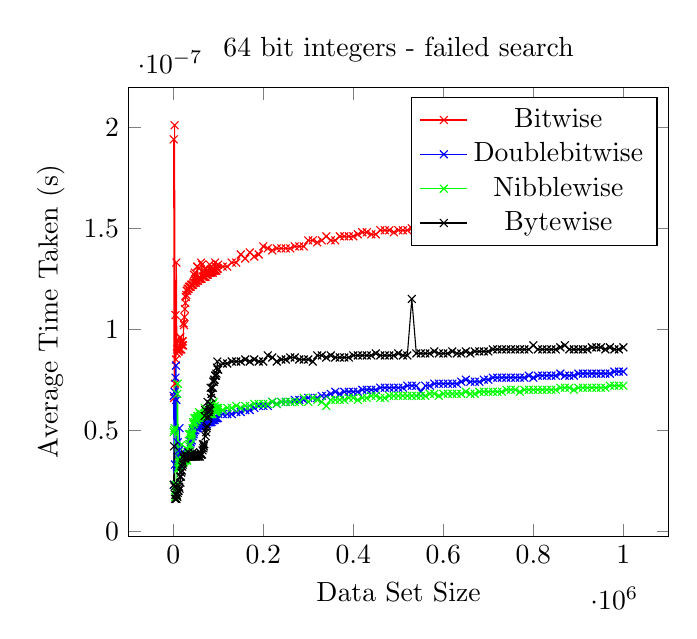
\begin{tikzpicture}
\begin{axis}[
xlabel=Data Set Size,
ylabel=Average Time Taken (s),
title=64 bit integers - failed search]
\addplot[color=red,mark=x] coordinates {
(1000,0.000000194
)
(2000,0.000000066
)
(3000,0.000000201
)
(4000,0.000000073
)
(5000,0.000000107
)
(6000,0.000000085
)
(7000,0.000000133
)
(8000,0.000000088
)
(9000,0.00000009
)
(10000,0.000000094
)
(11000,0.000000089
)
(12000,0.000000089
)
(13000,0.00000009
)
(14000,0.00000009
)
(15000,0.000000096
)
(16000,0.000000096
)
(17000,0.00000009
)
(18000,0.00000009
)
(19000,0.000000092
)
(20000,0.000000094
)
(21000,0.000000094
)
(22000,0.000000092
)
(23000,0.000000103
)
(24000,0.000000102
)
(25000,0.000000106
)
(26000,0.00000011
)
(27000,0.000000113
)
(28000,0.000000116
)
(29000,0.000000117
)
(30000,0.000000119
)
(31000,0.000000119
)
(32000,0.00000012
)
(33000,0.00000012
)
(34000,0.00000012
)
(35000,0.000000121
)
(36000,0.000000121
)
(37000,0.000000121
)
(38000,0.000000121
)
(39000,0.000000121
)
(40000,0.000000122
)
(41000,0.000000122
)
(42000,0.000000122
)
(43000,0.000000122
)
(44000,0.000000122
)
(45000,0.000000123
)
(46000,0.000000127
)
(47000,0.000000123
)
(48000,0.000000128
)
(49000,0.000000124
)
(50000,0.000000123
)
(51000,0.000000124
)
(52000,0.000000124
)
(53000,0.000000131
)
(54000,0.000000131
)
(55000,0.000000124
)
(56000,0.000000125
)
(57000,0.000000125
)
(58000,0.000000125
)
(59000,0.000000125
)
(60000,0.000000125
)
(61000,0.000000125
)
(62000,0.000000133
)
(63000,0.000000125
)
(64000,0.000000132
)
(65000,0.000000126
)
(66000,0.000000126
)
(67000,0.000000126
)
(68000,0.000000126
)
(69000,0.000000126
)
(70000,0.00000013
)
(71000,0.000000126
)
(72000,0.000000126
)
(73000,0.000000127
)
(74000,0.000000127
)
(75000,0.000000129
)
(76000,0.000000128
)
(77000,0.000000127
)
(78000,0.000000128
)
(79000,0.000000128
)
(80000,0.000000128
)
(81000,0.000000132
)
(82000,0.000000128
)
(83000,0.000000128
)
(84000,0.000000129
)
(85000,0.000000128
)
(86000,0.000000129
)
(87000,0.000000129
)
(88000,0.000000128
)
(89000,0.000000129
)
(90000,0.00000013
)
(91000,0.000000129
)
(92000,0.000000129
)
(93000,0.000000133
)
(94000,0.000000129
)
(95000,0.000000131
)
(96000,0.000000129
)
(97000,0.00000013
)
(98000,0.00000013
)
(99000,0.00000013
)
(100000,0.000000132
)
(110000,0.000000131
)
(120000,0.000000131
)
(130000,0.000000133
)
(140000,0.000000133
)
(150000,0.000000137
)
(160000,0.000000135
)
(170000,0.000000138
)
(180000,0.000000136
)
(190000,0.000000137
)
(200000,0.000000141
)
(210000,0.00000014
)
(220000,0.000000139
)
(230000,0.00000014
)
(240000,0.00000014
)
(250000,0.00000014
)
(260000,0.00000014
)
(270000,0.000000141
)
(280000,0.000000141
)
(290000,0.000000141
)
(300000,0.000000144
)
(310000,0.000000144
)
(320000,0.000000143
)
(330000,0.000000144
)
(340000,0.000000146
)
(350000,0.000000144
)
(360000,0.000000144
)
(370000,0.000000146
)
(380000,0.000000146
)
(390000,0.000000146
)
(400000,0.000000146
)
(410000,0.000000147
)
(420000,0.000000148
)
(430000,0.000000148
)
(440000,0.000000147
)
(450000,0.000000147
)
(460000,0.000000149
)
(470000,0.000000149
)
(480000,0.000000149
)
(490000,0.000000148
)
(500000,0.000000149
)
(510000,0.000000149
)
(520000,0.000000149
)
(530000,0.00000015
)
(540000,0.000000151
)
(550000,0.00000015
)
(560000,0.00000015
)
(570000,0.000000151
)
(580000,0.000000151
)
(590000,0.000000151
)
(600000,0.000000152
)
(610000,0.000000153
)
(620000,0.000000152
)
(630000,0.000000152
)
(640000,0.00000017
)
(650000,0.000000153
)
(660000,0.000000153
)
(670000,0.000000153
)
(680000,0.000000154
)
(690000,0.000000154
)
(700000,0.000000154
)
(710000,0.000000154
)
(720000,0.000000154
)
(730000,0.000000155
)
(740000,0.000000155
)
(750000,0.000000154
)
(760000,0.000000155
)
(770000,0.000000155
)
(780000,0.000000155
)
(790000,0.000000156
)
(800000,0.000000155
)
(810000,0.000000156
)
(820000,0.000000156
)
(830000,0.000000156
)
(840000,0.000000156
)
(850000,0.000000157
)
(860000,0.000000156
)
(870000,0.000000157
)
(880000,0.000000157
)
(890000,0.000000157
)
(900000,0.000000157
)
(910000,0.000000157
)
(920000,0.000000158
)
(930000,0.000000158
)
(940000,0.000000157
)
(950000,0.000000158
)
(960000,0.000000158
)
(970000,0.000000158
)
(980000,0.000000158
)
(990000,0.000000158
)
(1000000,0.000000158
)
};
\addlegendentry{Bitwise}
\addplot[color=blue,mark=x] coordinates {
(1000,0.000000067
)
(2000,0.000000023
)
(3000,0.000000069
)
(4000,0.000000033
)
(5000,0.000000076
)
(6000,0.000000082
)
(7000,0.000000065
)
(8000,0.000000032
)
(9000,0.000000031
)
(10000,0.000000044
)
(11000,0.000000033
)
(12000,0.000000035
)
(13000,0.00000004
)
(14000,0.000000051
)
(15000,0.000000034
)
(16000,0.000000034
)
(17000,0.000000036
)
(18000,0.000000035
)
(19000,0.000000035
)
(20000,0.000000036
)
(21000,0.000000035
)
(22000,0.000000036
)
(23000,0.000000036
)
(24000,0.000000036
)
(25000,0.000000036
)
(26000,0.000000037
)
(27000,0.000000036
)
(28000,0.000000037
)
(29000,0.000000037
)
(30000,0.000000038
)
(31000,0.000000038
)
(32000,0.000000039
)
(33000,0.000000038
)
(34000,0.000000038
)
(35000,0.000000039
)
(36000,0.000000039
)
(37000,0.000000048
)
(38000,0.000000043
)
(39000,0.000000044
)
(40000,0.000000045
)
(41000,0.000000045
)
(42000,0.000000047
)
(43000,0.000000047
)
(44000,0.00000005
)
(45000,0.000000048
)
(46000,0.000000049
)
(47000,0.00000005
)
(48000,0.00000005
)
(49000,0.00000005
)
(50000,0.000000053
)
(51000,0.000000051
)
(52000,0.000000052
)
(53000,0.000000051
)
(54000,0.000000051
)
(55000,0.000000051
)
(56000,0.000000052
)
(57000,0.000000052
)
(58000,0.000000052
)
(59000,0.000000056
)
(60000,0.000000052
)
(61000,0.000000052
)
(62000,0.000000052
)
(63000,0.000000053
)
(64000,0.000000052
)
(65000,0.000000053
)
(66000,0.000000053
)
(67000,0.000000053
)
(68000,0.000000053
)
(69000,0.000000053
)
(70000,0.000000054
)
(71000,0.000000053
)
(72000,0.000000057
)
(73000,0.000000054
)
(74000,0.000000053
)
(75000,0.000000053
)
(76000,0.000000054
)
(77000,0.000000054
)
(78000,0.000000054
)
(79000,0.000000054
)
(80000,0.000000054
)
(81000,0.000000054
)
(82000,0.000000054
)
(83000,0.000000055
)
(84000,0.000000054
)
(85000,0.000000054
)
(86000,0.000000055
)
(87000,0.000000055
)
(88000,0.000000055
)
(89000,0.000000055
)
(90000,0.000000056
)
(91000,0.000000056
)
(92000,0.000000055
)
(93000,0.000000056
)
(94000,0.000000056
)
(95000,0.000000056
)
(96000,0.000000056
)
(97000,0.000000056
)
(98000,0.000000056
)
(99000,0.000000056
)
(100000,0.000000058
)
(110000,0.000000058
)
(120000,0.000000058
)
(130000,0.000000058
)
(140000,0.000000059
)
(150000,0.000000059
)
(160000,0.00000006
)
(170000,0.00000006
)
(180000,0.000000061
)
(190000,0.000000062
)
(200000,0.000000062
)
(210000,0.000000062
)
(220000,0.000000064
)
(230000,0.000000063
)
(240000,0.000000064
)
(250000,0.000000064
)
(260000,0.000000064
)
(270000,0.000000065
)
(280000,0.000000065
)
(290000,0.000000065
)
(300000,0.000000066
)
(310000,0.000000066
)
(320000,0.000000066
)
(330000,0.000000067
)
(340000,0.000000067
)
(350000,0.000000068
)
(360000,0.000000069
)
(370000,0.000000068
)
(380000,0.000000069
)
(390000,0.000000069
)
(400000,0.000000069
)
(410000,0.000000069
)
(420000,0.00000007
)
(430000,0.00000007
)
(440000,0.00000007
)
(450000,0.00000007
)
(460000,0.000000071
)
(470000,0.000000071
)
(480000,0.000000071
)
(490000,0.000000071
)
(500000,0.000000071
)
(510000,0.000000071
)
(520000,0.000000072
)
(530000,0.000000072
)
(540000,0.000000072
)
(550000,0.000000069
)
(560000,0.000000072
)
(570000,0.000000072
)
(580000,0.000000073
)
(590000,0.000000073
)
(600000,0.000000073
)
(610000,0.000000073
)
(620000,0.000000073
)
(630000,0.000000073
)
(640000,0.000000074
)
(650000,0.000000075
)
(660000,0.000000074
)
(670000,0.000000074
)
(680000,0.000000074
)
(690000,0.000000075
)
(700000,0.000000075
)
(710000,0.000000076
)
(720000,0.000000076
)
(730000,0.000000076
)
(740000,0.000000076
)
(750000,0.000000076
)
(760000,0.000000076
)
(770000,0.000000076
)
(780000,0.000000076
)
(790000,0.000000077
)
(800000,0.000000076
)
(810000,0.000000077
)
(820000,0.000000077
)
(830000,0.000000077
)
(840000,0.000000077
)
(850000,0.000000077
)
(860000,0.000000078
)
(870000,0.000000077
)
(880000,0.000000077
)
(890000,0.000000077
)
(900000,0.000000078
)
(910000,0.000000078
)
(920000,0.000000078
)
(930000,0.000000078
)
(940000,0.000000078
)
(950000,0.000000078
)
(960000,0.000000078
)
(970000,0.000000078
)
(980000,0.000000079
)
(990000,0.000000079
)
(1000000,0.000000079
)
};
\addlegendentry{Doublebitwise}
\addplot[color=green,mark=x] coordinates {
(1000,0.000000049
)
(2000,0.00000005
)
(3000,0.000000051
)
(4000,0.000000017
)
(5000,0.000000018
)
(6000,0.000000023
)
(7000,0.000000019
)
(8000,0.000000022
)
(9000,0.000000068
)
(10000,0.000000073
)
(11000,0.000000031
)
(12000,0.000000032
)
(13000,0.000000034
)
(14000,0.000000033
)
(15000,0.000000035
)
(16000,0.000000034
)
(17000,0.000000034
)
(18000,0.000000034
)
(19000,0.000000043
)
(20000,0.000000034
)
(21000,0.000000035
)
(22000,0.000000035
)
(23000,0.000000034
)
(24000,0.000000035
)
(25000,0.000000035
)
(26000,0.000000035
)
(27000,0.000000036
)
(28000,0.000000036
)
(29000,0.000000036
)
(30000,0.000000035
)
(31000,0.000000035
)
(32000,0.000000037
)
(33000,0.000000038
)
(34000,0.00000004
)
(35000,0.000000048
)
(36000,0.000000042
)
(37000,0.000000043
)
(38000,0.000000048
)
(39000,0.000000046
)
(40000,0.000000047
)
(41000,0.000000048
)
(42000,0.000000049
)
(43000,0.000000051
)
(44000,0.000000054
)
(45000,0.000000053
)
(46000,0.000000053
)
(47000,0.000000056
)
(48000,0.000000054
)
(49000,0.000000056
)
(50000,0.000000055
)
(51000,0.000000055
)
(52000,0.000000055
)
(53000,0.000000056
)
(54000,0.000000057
)
(55000,0.000000057
)
(56000,0.000000056
)
(57000,0.000000059
)
(58000,0.000000056
)
(59000,0.000000057
)
(60000,0.000000058
)
(61000,0.000000057
)
(62000,0.000000057
)
(63000,0.000000058
)
(64000,0.000000057
)
(65000,0.000000057
)
(66000,0.000000057
)
(67000,0.000000057
)
(68000,0.000000057
)
(69000,0.000000057
)
(70000,0.000000061
)
(71000,0.000000058
)
(72000,0.000000057
)
(73000,0.000000058
)
(74000,0.000000058
)
(75000,0.000000058
)
(76000,0.000000058
)
(77000,0.000000058
)
(78000,0.000000058
)
(79000,0.000000058
)
(80000,0.000000058
)
(81000,0.000000058
)
(82000,0.000000059
)
(83000,0.000000058
)
(84000,0.00000006
)
(85000,0.000000058
)
(86000,0.000000058
)
(87000,0.000000058
)
(88000,0.000000063
)
(89000,0.000000061
)
(90000,0.000000064
)
(91000,0.00000006
)
(92000,0.000000062
)
(93000,0.000000059
)
(94000,0.000000061
)
(95000,0.00000006
)
(96000,0.000000059
)
(97000,0.000000059
)
(98000,0.000000061
)
(99000,0.00000006
)
(100000,0.000000061
)
(110000,0.00000006
)
(120000,0.000000061
)
(130000,0.000000061
)
(140000,0.000000062
)
(150000,0.000000061
)
(160000,0.000000062
)
(170000,0.000000062
)
(180000,0.000000063
)
(190000,0.000000063
)
(200000,0.000000063
)
(210000,0.000000063
)
(220000,0.000000064
)
(230000,0.000000063
)
(240000,0.000000064
)
(250000,0.000000064
)
(260000,0.000000064
)
(270000,0.000000064
)
(280000,0.000000064
)
(290000,0.000000066
)
(300000,0.000000064
)
(310000,0.000000066
)
(320000,0.000000065
)
(330000,0.000000064
)
(340000,0.000000062
)
(350000,0.000000065
)
(360000,0.000000065
)
(370000,0.000000065
)
(380000,0.000000065
)
(390000,0.000000066
)
(400000,0.000000066
)
(410000,0.000000065
)
(420000,0.000000066
)
(430000,0.000000066
)
(440000,0.000000067
)
(450000,0.000000067
)
(460000,0.000000066
)
(470000,0.000000066
)
(480000,0.000000067
)
(490000,0.000000067
)
(500000,0.000000067
)
(510000,0.000000067
)
(520000,0.000000067
)
(530000,0.000000067
)
(540000,0.000000067
)
(550000,0.000000067
)
(560000,0.000000067
)
(570000,0.000000068
)
(580000,0.000000068
)
(590000,0.000000067
)
(600000,0.000000068
)
(610000,0.000000068
)
(620000,0.000000068
)
(630000,0.000000068
)
(640000,0.000000068
)
(650000,0.000000069
)
(660000,0.000000068
)
(670000,0.000000068
)
(680000,0.000000069
)
(690000,0.000000069
)
(700000,0.000000069
)
(710000,0.000000069
)
(720000,0.000000069
)
(730000,0.000000069
)
(740000,0.00000007
)
(750000,0.00000007
)
(760000,0.00000007
)
(770000,0.000000069
)
(780000,0.00000007
)
(790000,0.00000007
)
(800000,0.00000007
)
(810000,0.00000007
)
(820000,0.00000007
)
(830000,0.00000007
)
(840000,0.00000007
)
(850000,0.00000007
)
(860000,0.000000071
)
(870000,0.000000071
)
(880000,0.000000071
)
(890000,0.00000007
)
(900000,0.000000071
)
(910000,0.000000071
)
(920000,0.000000071
)
(930000,0.000000071
)
(940000,0.000000071
)
(950000,0.000000071
)
(960000,0.000000071
)
(970000,0.000000072
)
(980000,0.000000072
)
(990000,0.000000072
)
(1000000,0.000000072
)
};
\addlegendentry{Nibblewise}
\addplot[color=black,mark=x] coordinates {
(1000,0.000000023
)
(2000,0.000000042
)
(3000,0.000000022
)
(4000,0.000000016
)
(5000,0.000000018
)
(6000,0.000000016
)
(7000,0.000000016
)
(8000,0.000000018
)
(9000,0.000000017
)
(10000,0.000000019
)
(11000,0.00000002
)
(12000,0.00000002
)
(13000,0.000000022
)
(14000,0.000000021
)
(15000,0.000000027
)
(16000,0.000000024
)
(17000,0.000000027
)
(18000,0.000000029
)
(19000,0.00000003
)
(20000,0.000000032
)
(21000,0.000000033
)
(22000,0.000000034
)
(23000,0.000000037
)
(24000,0.000000036
)
(25000,0.000000036
)
(26000,0.000000038
)
(27000,0.000000036
)
(28000,0.000000037
)
(29000,0.000000037
)
(30000,0.000000037
)
(31000,0.000000037
)
(32000,0.000000037
)
(33000,0.000000037
)
(34000,0.000000039
)
(35000,0.000000037
)
(36000,0.000000037
)
(37000,0.000000037
)
(38000,0.000000037
)
(39000,0.000000037
)
(40000,0.000000037
)
(41000,0.000000037
)
(42000,0.000000037
)
(43000,0.000000037
)
(44000,0.000000039
)
(45000,0.000000037
)
(46000,0.000000037
)
(47000,0.000000037
)
(48000,0.000000037
)
(49000,0.000000037
)
(50000,0.000000037
)
(51000,0.000000037
)
(52000,0.000000037
)
(53000,0.000000038
)
(54000,0.000000037
)
(55000,0.000000037
)
(56000,0.000000037
)
(57000,0.000000038
)
(58000,0.000000037
)
(59000,0.000000037
)
(60000,0.000000039
)
(61000,0.000000038
)
(62000,0.000000038
)
(63000,0.000000038
)
(64000,0.000000038
)
(65000,0.00000004
)
(66000,0.000000043
)
(67000,0.000000041
)
(68000,0.000000042
)
(69000,0.000000043
)
(70000,0.000000057
)
(71000,0.00000006
)
(72000,0.000000047
)
(73000,0.000000049
)
(74000,0.000000051
)
(75000,0.000000052
)
(76000,0.000000064
)
(77000,0.000000056
)
(78000,0.000000057
)
(79000,0.000000059
)
(80000,0.00000006
)
(81000,0.000000061
)
(82000,0.000000063
)
(83000,0.000000071
)
(84000,0.000000066
)
(85000,0.000000068
)
(86000,0.000000068
)
(87000,0.000000071
)
(88000,0.000000071
)
(89000,0.000000074
)
(90000,0.000000074
)
(91000,0.000000075
)
(92000,0.000000075
)
(93000,0.000000077
)
(94000,0.000000077
)
(95000,0.000000077
)
(96000,0.000000078
)
(97000,0.000000081
)
(98000,0.000000084
)
(99000,0.00000008
)
(100000,0.00000008
)
(110000,0.000000083
)
(120000,0.000000083
)
(130000,0.000000084
)
(140000,0.000000084
)
(150000,0.000000084
)
(160000,0.000000085
)
(170000,0.000000084
)
(180000,0.000000085
)
(190000,0.000000084
)
(200000,0.000000084
)
(210000,0.000000087
)
(220000,0.000000086
)
(230000,0.000000084
)
(240000,0.000000085
)
(250000,0.000000085
)
(260000,0.000000086
)
(270000,0.000000086
)
(280000,0.000000085
)
(290000,0.000000085
)
(300000,0.000000085
)
(310000,0.000000084
)
(320000,0.000000087
)
(330000,0.000000087
)
(340000,0.000000086
)
(350000,0.000000087
)
(360000,0.000000086
)
(370000,0.000000086
)
(380000,0.000000086
)
(390000,0.000000086
)
(400000,0.000000087
)
(410000,0.000000087
)
(420000,0.000000087
)
(430000,0.000000087
)
(440000,0.000000087
)
(450000,0.000000088
)
(460000,0.000000087
)
(470000,0.000000087
)
(480000,0.000000087
)
(490000,0.000000087
)
(500000,0.000000088
)
(510000,0.000000087
)
(520000,0.000000087
)
(530000,0.000000115
)
(540000,0.000000088
)
(550000,0.000000088
)
(560000,0.000000088
)
(570000,0.000000088
)
(580000,0.000000089
)
(590000,0.000000088
)
(600000,0.000000088
)
(610000,0.000000088
)
(620000,0.000000089
)
(630000,0.000000088
)
(640000,0.000000088
)
(650000,0.000000089
)
(660000,0.000000088
)
(670000,0.000000089
)
(680000,0.000000089
)
(690000,0.000000089
)
(700000,0.000000089
)
(710000,0.00000009
)
(720000,0.00000009
)
(730000,0.00000009
)
(740000,0.00000009
)
(750000,0.00000009
)
(760000,0.00000009
)
(770000,0.00000009
)
(780000,0.00000009
)
(790000,0.00000009
)
(800000,0.000000092
)
(810000,0.00000009
)
(820000,0.00000009
)
(830000,0.00000009
)
(840000,0.00000009
)
(850000,0.00000009
)
(860000,0.000000091
)
(870000,0.000000092
)
(880000,0.00000009
)
(890000,0.00000009
)
(900000,0.00000009
)
(910000,0.00000009
)
(920000,0.00000009
)
(930000,0.000000091
)
(940000,0.000000091
)
(950000,0.000000091
)
(960000,0.00000009
)
(970000,0.000000091
)
(980000,0.00000009
)
(990000,0.00000009
)
(1000000,0.000000091
)
};
\addlegendentry{Bytewise}
\end{axis}
\end{tikzpicture}

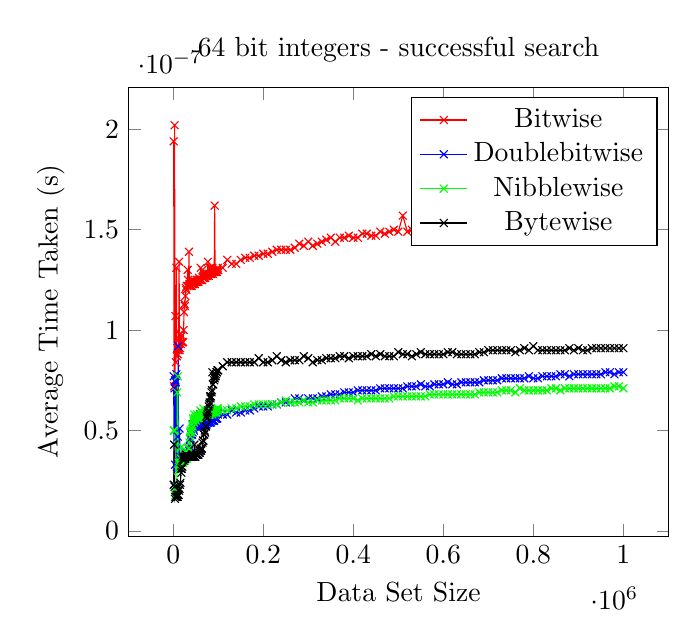
\begin{tikzpicture}
\begin{axis}[
xlabel=Data Set Size,
ylabel=Average Time Taken (s),
title=64 bit integers - successful search]
\addplot[color=red,mark=x] coordinates {
(1000,0.000000194)
(2000,0.000000072)
(3000,0.000000202)
(4000,0.000000075)
(5000,0.000000107)
(6000,0.000000084)
(7000,0.000000131)
(8000,0.000000087)
(9000,0.000000091)
(10000,0.000000088)
(11000,0.00000009)
(12000,0.000000091)
(13000,0.000000134)
(14000,0.00000009)
(15000,0.000000091)
(16000,0.000000098)
(17000,0.000000093)
(18000,0.000000097)
(19000,0.000000094)
(20000,0.000000094)
(21000,0.000000094)
(22000,0.000000094)
(23000,0.0000001)
(24000,0.000000109)
(25000,0.000000113)
(26000,0.000000112)
(27000,0.000000117)
(28000,0.000000121)
(29000,0.00000012)
(30000,0.000000122)
(31000,0.000000122)
(32000,0.00000013)
(33000,0.000000125)
(34000,0.000000122)
(35000,0.000000139)
(36000,0.000000123)
(37000,0.000000122)
(38000,0.000000123)
(39000,0.000000124)
(40000,0.000000122)
(41000,0.000000122)
(42000,0.000000123)
(43000,0.000000124)
(44000,0.000000123)
(45000,0.000000123)
(46000,0.000000123)
(47000,0.000000124)
(48000,0.000000123)
(49000,0.000000124)
(50000,0.000000124)
(51000,0.000000124)
(52000,0.000000125)
(53000,0.000000124)
(54000,0.000000125)
(55000,0.000000124)
(56000,0.000000124)
(57000,0.000000126)
(58000,0.000000125)
(59000,0.000000125)
(60000,0.000000125)
(61000,0.000000131)
(62000,0.000000125)
(63000,0.000000125)
(64000,0.000000125)
(65000,0.00000013)
(66000,0.000000126)
(67000,0.000000126)
(68000,0.000000126)
(69000,0.000000127)
(70000,0.000000126)
(71000,0.000000126)
(72000,0.000000127)
(73000,0.000000127)
(74000,0.000000127)
(75000,0.000000127)
(76000,0.000000127)
(77000,0.000000134)
(78000,0.000000128)
(79000,0.000000127)
(80000,0.000000128)
(81000,0.000000131)
(82000,0.000000128)
(83000,0.000000131)
(84000,0.000000128)
(85000,0.000000128)
(86000,0.000000129)
(87000,0.000000131)
(88000,0.000000128)
(89000,0.000000129)
(90000,0.000000129)
(91000,0.000000129)
(92000,0.000000162)
(93000,0.000000129)
(94000,0.000000129)
(95000,0.000000129)
(96000,0.00000013)
(97000,0.000000129)
(98000,0.00000013)
(99000,0.000000131)
(100000,0.00000013)
(110000,0.000000131)
(120000,0.000000135)
(130000,0.000000133)
(140000,0.000000133)
(150000,0.000000135)
(160000,0.000000136)
(170000,0.000000136)
(180000,0.000000137)
(190000,0.000000137)
(200000,0.000000138)
(210000,0.000000138)
(220000,0.000000139)
(230000,0.00000014)
(240000,0.00000014)
(250000,0.00000014)
(260000,0.00000014)
(270000,0.000000141)
(280000,0.000000143)
(290000,0.000000142)
(300000,0.000000144)
(310000,0.000000142)
(320000,0.000000143)
(330000,0.000000144)
(340000,0.000000145)
(350000,0.000000146)
(360000,0.000000144)
(370000,0.000000146)
(380000,0.000000146)
(390000,0.000000147)
(400000,0.000000146)
(410000,0.000000146)
(420000,0.000000148)
(430000,0.000000148)
(440000,0.000000147)
(450000,0.000000147)
(460000,0.000000149)
(470000,0.000000148)
(480000,0.000000149)
(490000,0.00000015)
(500000,0.000000149)
(510000,0.000000157)
(520000,0.000000149)
(530000,0.00000015)
(540000,0.000000151)
(550000,0.00000015)
(560000,0.00000015)
(570000,0.00000015)
(580000,0.000000151)
(590000,0.000000152)
(600000,0.000000152)
(610000,0.000000152)
(620000,0.000000152)
(630000,0.000000153)
(640000,0.000000152)
(650000,0.000000153)
(660000,0.000000152)
(670000,0.000000153)
(680000,0.000000154)
(690000,0.000000154)
(700000,0.000000154)
(710000,0.000000154)
(720000,0.000000154)
(730000,0.000000154)
(740000,0.000000155)
(750000,0.000000155)
(760000,0.000000155)
(770000,0.000000155)
(780000,0.000000155)
(790000,0.000000156)
(800000,0.000000155)
(810000,0.000000155)
(820000,0.000000156)
(830000,0.000000156)
(840000,0.000000156)
(850000,0.000000156)
(860000,0.000000157)
(870000,0.000000156)
(880000,0.000000157)
(890000,0.000000157)
(900000,0.000000158)
(910000,0.000000157)
(920000,0.000000157)
(930000,0.000000158)
(940000,0.000000158)
(950000,0.000000158)
(960000,0.000000158)
(970000,0.000000159)
(980000,0.000000158)
(990000,0.000000158)
(1000000,0.000000158)
};
\addlegendentry{Bitwise}
\addplot[color=blue,mark=x] coordinates {
(1000,0.000000077)
(2000,0.000000023)
(3000,0.000000071)
(4000,0.000000033)
(5000,0.000000075)
(6000,0.000000074)
(7000,0.000000078)
(8000,0.000000032)
(9000,0.000000031)
(10000,0.000000047)
(11000,0.000000092)
(12000,0.000000033)
(13000,0.000000034)
(14000,0.000000051)
(15000,0.000000037)
(16000,0.000000036)
(17000,0.000000035)
(18000,0.000000035)
(19000,0.000000035)
(20000,0.000000035)
(21000,0.000000036)
(22000,0.000000036)
(23000,0.000000036)
(24000,0.000000037)
(25000,0.000000036)
(26000,0.000000036)
(27000,0.000000036)
(28000,0.000000039)
(29000,0.000000037)
(30000,0.000000039)
(31000,0.000000037)
(32000,0.000000037)
(33000,0.000000039)
(34000,0.000000041)
(35000,0.00000004)
(36000,0.000000041)
(37000,0.000000042)
(38000,0.000000046)
(39000,0.000000046)
(40000,0.000000048)
(41000,0.000000048)
(42000,0.000000048)
(43000,0.000000049)
(44000,0.000000053)
(45000,0.000000051)
(46000,0.00000005)
(47000,0.000000052)
(48000,0.000000052)
(49000,0.000000056)
(50000,0.000000053)
(51000,0.000000052)
(52000,0.000000053)
(53000,0.000000054)
(54000,0.000000052)
(55000,0.000000053)
(56000,0.000000052)
(57000,0.000000052)
(58000,0.000000052)
(59000,0.000000052)
(60000,0.000000058)
(61000,0.000000052)
(62000,0.000000052)
(63000,0.000000057)
(64000,0.000000053)
(65000,0.000000053)
(66000,0.000000053)
(67000,0.000000053)
(68000,0.000000053)
(69000,0.000000053)
(70000,0.000000054)
(71000,0.000000053)
(72000,0.000000053)
(73000,0.000000053)
(74000,0.000000053)
(75000,0.000000054)
(76000,0.000000054)
(77000,0.000000054)
(78000,0.000000054)
(79000,0.000000056)
(80000,0.000000055)
(81000,0.000000054)
(82000,0.000000054)
(83000,0.000000056)
(84000,0.000000054)
(85000,0.000000055)
(86000,0.000000055)
(87000,0.000000055)
(88000,0.000000055)
(89000,0.000000055)
(90000,0.000000055)
(91000,0.000000055)
(92000,0.00000006)
(93000,0.000000056)
(94000,0.000000056)
(95000,0.000000056)
(96000,0.000000056)
(97000,0.000000056)
(98000,0.000000056)
(99000,0.000000058)
(100000,0.000000059)
(110000,0.000000058)
(120000,0.000000058)
(130000,0.00000006)
(140000,0.000000059)
(150000,0.000000059)
(160000,0.00000006)
(170000,0.00000006)
(180000,0.000000061)
(190000,0.000000062)
(200000,0.000000062)
(210000,0.000000062)
(220000,0.000000063)
(230000,0.000000063)
(240000,0.000000064)
(250000,0.000000064)
(260000,0.000000064)
(270000,0.000000066)
(280000,0.000000066)
(290000,0.000000065)
(300000,0.000000066)
(310000,0.000000066)
(320000,0.000000066)
(330000,0.000000067)
(340000,0.000000067)
(350000,0.000000068)
(360000,0.000000068)
(370000,0.000000068)
(380000,0.000000069)
(390000,0.000000069)
(400000,0.000000069)
(410000,0.00000007)
(420000,0.00000007)
(430000,0.00000007)
(440000,0.00000007)
(450000,0.00000007)
(460000,0.000000071)
(470000,0.000000071)
(480000,0.000000071)
(490000,0.000000071)
(500000,0.000000071)
(510000,0.000000071)
(520000,0.000000072)
(530000,0.000000072)
(540000,0.000000072)
(550000,0.000000073)
(560000,0.000000072)
(570000,0.000000072)
(580000,0.000000073)
(590000,0.000000073)
(600000,0.000000073)
(610000,0.000000074)
(620000,0.000000073)
(630000,0.000000073)
(640000,0.000000074)
(650000,0.000000074)
(660000,0.000000074)
(670000,0.000000074)
(680000,0.000000074)
(690000,0.000000075)
(700000,0.000000075)
(710000,0.000000075)
(720000,0.000000075)
(730000,0.000000076)
(740000,0.000000076)
(750000,0.000000076)
(760000,0.000000076)
(770000,0.000000076)
(780000,0.000000076)
(790000,0.000000077)
(800000,0.000000076)
(810000,0.000000076)
(820000,0.000000077)
(830000,0.000000077)
(840000,0.000000077)
(850000,0.000000077)
(860000,0.000000078)
(870000,0.000000078)
(880000,0.000000077)
(890000,0.000000078)
(900000,0.000000078)
(910000,0.000000078)
(920000,0.000000078)
(930000,0.000000078)
(940000,0.000000078)
(950000,0.000000078)
(960000,0.000000079)
(970000,0.000000079)
(980000,0.000000078)
(990000,0.000000079)
(1000000,0.000000079)
};
\addlegendentry{Doublebitwise}
\addplot[color=green,mark=x] coordinates {
(1000,0.00000005)
(2000,0.00000005)
(3000,0.00000005)
(4000,0.000000017)
(5000,0.000000018)
(6000,0.000000018)
(7000,0.000000019)
(8000,0.000000022)
(9000,0.000000069)
(10000,0.000000077)
(11000,0.00000003)
(12000,0.000000034)
(13000,0.000000032)
(14000,0.000000033)
(15000,0.000000034)
(16000,0.000000034)
(17000,0.000000036)
(18000,0.000000034)
(19000,0.000000042)
(20000,0.000000034)
(21000,0.000000036)
(22000,0.000000034)
(23000,0.000000036)
(24000,0.000000036)
(25000,0.000000035)
(26000,0.000000035)
(27000,0.000000039)
(28000,0.000000037)
(29000,0.000000038)
(30000,0.000000037)
(31000,0.000000036)
(32000,0.000000039)
(33000,0.000000039)
(34000,0.000000041)
(35000,0.000000041)
(36000,0.000000044)
(37000,0.000000049)
(38000,0.000000047)
(39000,0.00000005)
(40000,0.000000049)
(41000,0.000000051)
(42000,0.000000053)
(43000,0.000000052)
(44000,0.000000056)
(45000,0.000000055)
(46000,0.000000054)
(47000,0.000000058)
(48000,0.000000056)
(49000,0.000000056)
(50000,0.000000055)
(51000,0.000000057)
(52000,0.000000057)
(53000,0.000000058)
(54000,0.000000056)
(55000,0.000000057)
(56000,0.000000057)
(57000,0.000000056)
(58000,0.000000056)
(59000,0.000000056)
(60000,0.00000006)
(61000,0.000000058)
(62000,0.000000058)
(63000,0.000000059)
(64000,0.000000057)
(65000,0.000000057)
(66000,0.000000058)
(67000,0.000000061)
(68000,0.000000058)
(69000,0.000000057)
(70000,0.000000058)
(71000,0.000000058)
(72000,0.000000058)
(73000,0.000000058)
(74000,0.000000058)
(75000,0.000000058)
(76000,0.000000058)
(77000,0.000000058)
(78000,0.000000058)
(79000,0.000000058)
(80000,0.000000058)
(81000,0.000000058)
(82000,0.000000059)
(83000,0.000000059)
(84000,0.00000006)
(85000,0.000000061)
(86000,0.000000059)
(87000,0.000000058)
(88000,0.00000006)
(89000,0.000000059)
(90000,0.000000059)
(91000,0.00000006)
(92000,0.000000059)
(93000,0.00000006)
(94000,0.000000059)
(95000,0.000000059)
(96000,0.000000059)
(97000,0.000000061)
(98000,0.00000006)
(99000,0.000000061)
(100000,0.00000006)
(110000,0.00000006)
(120000,0.00000006)
(130000,0.000000061)
(140000,0.000000061)
(150000,0.000000062)
(160000,0.000000062)
(170000,0.000000062)
(180000,0.000000063)
(190000,0.000000063)
(200000,0.000000063)
(210000,0.000000063)
(220000,0.000000063)
(230000,0.000000063)
(240000,0.000000064)
(250000,0.000000065)
(260000,0.000000064)
(270000,0.000000064)
(280000,0.000000064)
(290000,0.000000065)
(300000,0.000000064)
(310000,0.000000064)
(320000,0.000000065)
(330000,0.000000065)
(340000,0.000000065)
(350000,0.000000065)
(360000,0.000000065)
(370000,0.000000066)
(380000,0.000000066)
(390000,0.000000066)
(400000,0.000000066)
(410000,0.000000065)
(420000,0.000000066)
(430000,0.000000066)
(440000,0.000000066)
(450000,0.000000066)
(460000,0.000000066)
(470000,0.000000066)
(480000,0.000000066)
(490000,0.000000067)
(500000,0.000000067)
(510000,0.000000067)
(520000,0.000000067)
(530000,0.000000067)
(540000,0.000000067)
(550000,0.000000067)
(560000,0.000000067)
(570000,0.000000068)
(580000,0.000000068)
(590000,0.000000068)
(600000,0.000000068)
(610000,0.000000068)
(620000,0.000000068)
(630000,0.000000068)
(640000,0.000000068)
(650000,0.000000068)
(660000,0.000000068)
(670000,0.000000068)
(680000,0.000000069)
(690000,0.000000069)
(700000,0.000000069)
(710000,0.000000069)
(720000,0.000000069)
(730000,0.00000007)
(740000,0.00000007)
(750000,0.00000007)
(760000,0.000000069)
(770000,0.000000071)
(780000,0.00000007)
(790000,0.00000007)
(800000,0.00000007)
(810000,0.00000007)
(820000,0.00000007)
(830000,0.00000007)
(840000,0.000000071)
(850000,0.000000071)
(860000,0.00000007)
(870000,0.000000071)
(880000,0.000000071)
(890000,0.000000071)
(900000,0.000000071)
(910000,0.000000071)
(920000,0.000000071)
(930000,0.000000071)
(940000,0.000000071)
(950000,0.000000071)
(960000,0.000000071)
(970000,0.000000071)
(980000,0.000000072)
(990000,0.000000072)
(1000000,0.000000071)
};
\addlegendentry{Nibblewise}
\addplot[color=black,mark=x] coordinates {
(1000,0.000000023)
(2000,0.000000043)
(3000,0.000000022)
(4000,0.000000016)
(5000,0.000000017)
(6000,0.000000017)
(7000,0.000000017)
(8000,0.000000018)
(9000,0.000000017)
(10000,0.000000017)
(11000,0.000000018)
(12000,0.000000018)
(13000,0.00000002)
(14000,0.000000021)
(15000,0.000000023)
(16000,0.000000024)
(17000,0.000000031)
(18000,0.000000029)
(19000,0.000000031)
(20000,0.000000032)
(21000,0.000000037)
(22000,0.000000036)
(23000,0.000000035)
(24000,0.000000036)
(25000,0.000000037)
(26000,0.000000036)
(27000,0.000000037)
(28000,0.000000038)
(29000,0.000000038)
(30000,0.000000037)
(31000,0.000000037)
(32000,0.000000037)
(33000,0.000000037)
(34000,0.000000037)
(35000,0.000000037)
(36000,0.000000037)
(37000,0.000000037)
(38000,0.000000037)
(39000,0.000000037)
(40000,0.000000037)
(41000,0.000000038)
(42000,0.000000037)
(43000,0.000000037)
(44000,0.000000037)
(45000,0.000000038)
(46000,0.000000037)
(47000,0.000000043)
(48000,0.000000037)
(49000,0.000000037)
(50000,0.000000038)
(51000,0.000000038)
(52000,0.000000038)
(53000,0.000000038)
(54000,0.000000038)
(55000,0.000000038)
(56000,0.000000038)
(57000,0.000000039)
(58000,0.00000004)
(59000,0.000000039)
(60000,0.00000004)
(61000,0.000000041)
(62000,0.00000004)
(63000,0.000000041)
(64000,0.000000041)
(65000,0.000000044)
(66000,0.000000045)
(67000,0.000000045)
(68000,0.000000048)
(69000,0.000000048)
(70000,0.00000005)
(71000,0.000000049)
(72000,0.000000052)
(73000,0.000000052)
(74000,0.000000057)
(75000,0.000000056)
(76000,0.000000058)
(77000,0.000000059)
(78000,0.00000006)
(79000,0.000000062)
(80000,0.000000063)
(81000,0.000000064)
(82000,0.000000067)
(83000,0.000000066)
(84000,0.000000067)
(85000,0.000000069)
(86000,0.00000007)
(87000,0.000000079)
(88000,0.000000073)
(89000,0.000000073)
(90000,0.000000077)
(91000,0.000000075)
(92000,0.000000076)
(93000,0.000000077)
(94000,0.000000077)
(95000,0.000000078)
(96000,0.000000079)
(97000,0.000000079)
(98000,0.00000008)
(99000,0.00000008)
(100000,0.00000008)
(110000,0.000000082)
(120000,0.000000084)
(130000,0.000000084)
(140000,0.000000084)
(150000,0.000000084)
(160000,0.000000084)
(170000,0.000000084)
(180000,0.000000084)
(190000,0.000000086)
(200000,0.000000084)
(210000,0.000000084)
(220000,0.000000085)
(230000,0.000000087)
(240000,0.000000085)
(250000,0.000000084)
(260000,0.000000085)
(270000,0.000000085)
(280000,0.000000085)
(290000,0.000000087)
(300000,0.000000086)
(310000,0.000000084)
(320000,0.000000085)
(330000,0.000000085)
(340000,0.000000086)
(350000,0.000000086)
(360000,0.000000086)
(370000,0.000000087)
(380000,0.000000087)
(390000,0.000000086)
(400000,0.000000087)
(410000,0.000000087)
(420000,0.000000087)
(430000,0.000000087)
(440000,0.000000088)
(450000,0.000000087)
(460000,0.000000088)
(470000,0.000000087)
(480000,0.000000087)
(490000,0.000000087)
(500000,0.000000089)
(510000,0.000000088)
(520000,0.000000088)
(530000,0.000000087)
(540000,0.000000088)
(550000,0.000000089)
(560000,0.000000088)
(570000,0.000000088)
(580000,0.000000088)
(590000,0.000000088)
(600000,0.000000088)
(610000,0.000000089)
(620000,0.000000089)
(630000,0.000000088)
(640000,0.000000088)
(650000,0.000000088)
(660000,0.000000088)
(670000,0.000000088)
(680000,0.000000089)
(690000,0.000000089)
(700000,0.00000009)
(710000,0.00000009)
(720000,0.00000009)
(730000,0.00000009)
(740000,0.00000009)
(750000,0.00000009)
(760000,0.000000089)
(770000,0.00000009)
(780000,0.000000091)
(790000,0.00000009)
(800000,0.000000092)
(810000,0.00000009)
(820000,0.00000009)
(830000,0.00000009)
(840000,0.00000009)
(850000,0.00000009)
(860000,0.00000009)
(870000,0.00000009)
(880000,0.000000091)
(890000,0.00000009)
(900000,0.000000091)
(910000,0.00000009)
(920000,0.00000009)
(930000,0.000000091)
(940000,0.000000091)
(950000,0.000000091)
(960000,0.000000091)
(970000,0.000000091)
(980000,0.000000091)
(990000,0.000000091)
(1000000,0.000000091)

};
\addlegendentry{Bytewise}

\end{axis}
\end{tikzpicture}

 %modified plots.tex that is no longer standalone
\newpage
Since we used unique integers, each insert traversed the same number of nodes for each insert operation. On the other hand, while in the ``success" case, the trie may have needed to be extended to hold parts of the string, this was never an issue for the ``failure" case (since the string to be inserted already existed in the trie). As can be seen in the next four charts, there are a few patterns to the data: most notably, the nibblewise and doublebitwise tries had the best performance, with the nibblewise trie coming out on top. The bytewise and bitwise tries had worse performance than the two trie types already mentioned, but on failed inserts (where the element was already in the trie), the bytewise trie pulled aheaad of the bitwise trie (and started to pull ahead of the doublebitwise trie). However, the opposite was true for the successful insert, where the bytewise trie was the worst performer.\\
\includegraphics[width=\linewidth,height=0.5\linewidth]{32_successful_insert.tex.tikz}
\includegraphics[width=\linewidth,height=0.5\linewidth]{64_successful_insert.tex.tikz}
\includegraphics[width=\linewidth,height=0.5\linewidth]{32_failed_insert.tex.tikz}
\includegraphics[width=\linewidth,height=0.5\linewidth]{64_failed_insert.tex.tikz}

\newpage
On searches, the code is able to kick out of the traversal of the trie when a single character from the target string is not found, so the time consumed on a failed search is bounded from above by the time consumed by the insert function, or by successful searches, which would also have to traverse the entire string's length in the trie. The results on the next four charts concerning searches are similar to the previous results on inserts. Again, the nibblewise and doublebitwise tries had the best performance, with the nibblewise trie winning out. However, unlike in the insert case, the bitwise trie never beat the bytewise trie in any experiment, and in fact was the worst performer overall in the search experiment scenarios.\\
\includegraphics[width=\linewidth,height=0.5\linewidth]{32_successful_search.tex.tikz}
\includegraphics[width=\linewidth,height=0.5\linewidth]{64_successful_search.tex.tikz}
\includegraphics[width=\linewidth,height=0.5\linewidth]{32_failed_search.tex.tikz}
\includegraphics[width=\linewidth,height=0.5\linewidth]{64_failed_search.tex.tikz}

\newpage
Similar to the search case, the delete operation on tries is able to drop out of the operation early when part of a string that is searched for is not found. As one can see in the next four charts, the results are the same as in the case of the searches: the nibblewise and doublebitwise tries performed the best, with the nibblewise trie pulling ahead, and the bitwise trie performed the worst overall. The fact that the search and delete scenarios had very similar results is as expected - since their operations are almost identical, there should not be a difference in the observed performance.\\
\includegraphics[width=\linewidth,height=0.5\linewidth]{32_successful_delete.tex.tikz}
\includegraphics[width=\linewidth,height=0.5\linewidth]{64_successful_delete.tex.tikz}
\includegraphics[width=\linewidth,height=0.5\linewidth]{32_failed_delete.tex.tikz}
\includegraphics[width=\linewidth,height=0.5\linewidth]{64_failed_delete.tex.tikz}

\newpage
From the plots, it is easy to see that although each trie theoretically should perform roughly equivalently (as mentioned previously), the choice of spread causes different behavior in terms of time consumed. Specifically, the trie that considered input string in terms of four bit (nibble-sized) chunks performed the best. This is unexpected - one would think that either extreme (the bitwise or bytewise tries) would perform the best due to the structure of the trie implied by the node size, and the other trie types would gradually perform worse as we increased or decreased the chunk size considered by each node. One possible explanation is that the overhead consumed by the structure around the trie nodes (which was constant across all types) was enough to slow down the bitwise and doublebitwise implementations of the trie, but not enough to slow down the nibblewise trie, which was able to outperform the bytewise trie for other reasons, like those mentioned below.\\
\section{Conclusion and discussion}
In terms of the performance, it's possible that the generated code / CPU cache size was such that it favored the trie whose chunk size was four bits, but that is beyond the scope of this paper. It's also possible that other CPUs would exhibit different behavior (for reference, these data points were generated on a computer built around an AMD FX-6300 CPU, with enough memory such that memory paging out to disk was not an issue during the experiment). This would also explain why the nibblewise trie outperformed the bytewise trie, even though the bytewise trie would have had the least structural overhead of the trie types that were experimented with, due to the breadth over depth approach the bytewise trie would use compared to the depth over breadth approach the bitwise trie uses.\\
One alteration that might be interesting to look at in tries is the use of other trie techniques, like compression of common paths, but this would require adapting those techniques to take into account the different chunk size used by each of the tries in the library above. Compression of common paths would merge common infixes and suffixes as the trie does now with prefixes, with the added computational complexity that would be created to account for the change in the algorithm.\\
Finally, there is also a CPU intrinsic instruction that could be harnessed to further speed actions against the trie up, called Count Leading Zeroes (CLZ). Use of this instruction would allow the algorithm to first examine the input string, find the first set bit, and jump that far down in the trie, rather than having to manually walk through the path of zeroes. This approach would keep track of paths in the trie composed entirely of leading zeroes to facilitate this purpose, which would only require storage size linear with respect to the number of bits stored in the longest string in the trie. \\
%TODO mention that using a custom allocator (bins holding blocks of the size of the node) might speed this up even more.
\newpage
%\ttdefault
\section{Manual Page}
%TODO make this in monospace, like a real man page!
\noindent NAME

make\_trie, trie\_insert, trie\_delete, trie\_search - Create and interact with tries.\\

\noindent SYNOPSIS

Trie *make\_trie(enum trie\_type type);\\
\indent int trie\_insert(Trie *t, void *item, int sz);\\
\indent int trie\_delete(Trie *t, void *item, int sz);\\
\indent int trie\_search(Trie *t, void *item, int sz);\\

\noindent DESCRIPTION

\noindent The make\_trie() function creates a trie struct in memory and returns a pointer to it. The type of trie (the branching factor) must be specified as one of the following enumerated values: BIT, DBLBIT, NIBBLE, BYTE.\\
The trie\_insert() function takes the data of length sz bytes which is pointed to by item and attempts to insert it into the trie t.\\
The trie\_delete() function takes the data of length sz bytes which is pointed to by item and attempts to remove it from the trie t.\\
The trie\_search() function takes the data of length sz bytes which is pointed to by item and attempts to find it in the trie t.\\

\noindent RETURN VALUE

\noindent The return value of make\_trie() is a pointer to a struct of type Trie which is suitable for use with the trie\_insert, trie\_delete, and trie\_search functions.\\
The trie\_insert function returns 1 when the specified value is inserted into the given trie and 0 when the specified value is already in the tree.\\
The trie\_delete function returns 1 when the specified value is removed from the given trie and 0 when the specified value is not already in the tree to remove.\\
The trie\_search function returns 1 when the specified value is found in the given trie and 0 if the specified value is not found.\\

\newpage
\section{Code}
\lstinputlisting[label=header, caption=trie.h, language=C, breaklines=true]{trie.h}
\newpage
\lstinputlisting[label=code, caption=trie.c, language=C, breaklines=true]{trie.c}

\end{document}
